\chapter{Results - Person specific}
{\samenvatting todo}

\section{Used approach}
\label{approach}

The first part of this work is looking at features in a person specific setting. This means that the algorithm is trained and tested on data from the same person. The main goals was to find features that give insight in the arousal and valence state of a person. To do so, each sample is labelled using a simple binary classification. Given that the dimension range from 1 to 9, all labels with a valence or arousal below 5 were reported as low valence or arousal respectively. The remaining valence or arousal were placed in the high valence or arousal respectively.

\npar

This thesis compares the aforementioned features and feature selection methods. For this a two stepped algorithm, inspired by the advanced random forest method, explained in Section \ref{rfmethod}, was used. In short, the first step is to rank all the features and only take the top X of the features. This threshold is applied to limit computation times and cancel features with low or zero importance. The next step is to build a model by selecting features out of the remaining feature set. This approach is depicted in Figure \ref{flow}.

\mijnfiguur{width=0.9\textwidth}{flow}{The used approach of this thesis.}

As you can see in Figure \ref{flow}, the approach starts by separating a test set to evaluate the final performance of the algorithm. This test set contains 10 of the 40 samples. Next, the aforementioned feature selection methods are applied to the train set. A top $X$ of the features is then kept, all other features are cancelled.

\npar

In the next step a model is build with the selected features. This is done iteratively by starting with an empty feature set. In the add step, a feature is added to this set and the cross validation error is determined. Cross validation is a technique that separates the data in N folds, as shown in Figure \ref{CVscheme}. The algorithm is then trained on N-1 blocks and tested on the remaining blocks. This is done N times and the average of the performance is then reported as cross validation error. 

%CV fig
\mijnfiguur{width=0.55\textwidth}{CVscheme}{Cross validation}

The advantage of using a cross validation scheme is that it gives a good estimation of the generalisation of the algorithm. This step is important because it ensures that chosen features have good generalisation properties. This avoids overfitting on the train set and ensure that the features will still work for unseen samples. Note that the test set, displayed in red, is not used during cross validation. The test set is kept completely separate to ensure that a fair estimate of the generalisation is achieved.

\npar

Next the average of the cross validation errors and the standard deviation is calculated. The average cross validation minus the standard deviation is then compared to the previous best performance. If the performance is better, the feature is kept in the feature set. If the performance is not better, the feature is neglected. This is repeated for all the features. 

\npar

The standard deviation is included to increase the stability of the algorithm. By making sure that the new model performs better in a statistical way, one can avoid that small differences in averages lead to a different model. In other words, the standard deviation makes the algorithm more stable.

\npar

In the final step the performance of the test set is determined by the accuracy metric. Accuracy is chosen as metric, because this metric gives a clear and intuitive measurement of performance.

\npar

The first parameter of this flow is the threshold parameter, indicated in the figure as $X$. This threshold cancels features with low importance, by simply taking the best $X$ features from the feature ranking. Assigning a high value to the threshold will increase calculation times as more features are available for the building phase. The performance of the model, will not be better though. Most of the additional features will have low importance values and are not likely to improve performance. Setting a low threshold might cancel out important features. 

\npar

In this work, the parameter was fixed to 30 for all feature selection methods for the following two reasons. First, considering that there are 30 samples in the feature set, having 30 features is already more than enough. Note that a well-known rule of thumb is to have at least 10 times more samples than features\citep{rot1,rot2}\footnote{Note that this is just a rule of thumb, and therefore not proven theoretically. In practice however, it turns out to work quite well.}. Second, looking at the features that were selected during training, one can see that usually around 5-7 features remain. The last selected feature usually has a rank around 20, meaning that the last 10 available features in the building phase are rarely used.

\npar
A second parameter of this model is a model to estimate the performance. For this, an SVM with a radial basis functions (RBF)\nomenclature{RBF}{Radial Basis Functions} kernel is used as model. This model was chosen because it has proven itself in multiple emotion recognition studies\citep{killyPaper,emorecoghard}. Additionally, SVMs are capable to handle small datasets. SVMs look for a separation boundary between two classes, and thus only look at points close to that border. This gives this method an advantage in this experiment, as the dataset only contains 40 samples for each person, only 30 of them are available for training. The RBF kernel was chosen, because the assumption is made that similar emotions lie close to each other. 

\npar

Some feature selection methods use a machine learning technique as basis. These methods were not used in the final building phase. This was done because some underlying methods are actually regression algorithms, meaning that they will produce a continuous output. This is in contrast with the classification problem that is solved in this work\footnote{Several tests in the early stage of this work indicated that even though continuous valence and arousal values are available, classification was more designated.}. To ensure that all final models were capable of classification, one classification model was used in the final step. This ensures that the comparison between feature selection methods was possible.

\section{Performance}

When looking at the accuracies of the different feature selection models in combination with the SVM, it is clear that there is not a lot of difference. Statistically, all these results are equivalent.
For each feature selection method, the test accuracy and standard deviation are shown in Table \ref{accCompLblarousal} and Table \ref{accCompLblvalence} for valence and arousal respectively. The accuracies are also plotted in in Figure \ref{accComp_arousalSVM} and Figure \ref{accComp_valenceSVM} for arousal and valence respectively.

\mijnfiguur{width=1.\textwidth}{accComp_arousalSVM}{Comparison of different feature selection methods for arousal recognition. The blue bars correspond to filter selection methods. Red bars correspond to wrapper methods and green bars are used for the embedded methods.}

\begin{table}[H]
\centering
\begin{tabular}{llll}
\textbf{Number} & \textbf{Feature selection method} & \textbf{Avg test acc - arousal} & \textbf{Std test acc - arousal} \\ \hline
0               & pearson                           & 0.68125                             & 0.1615199978                    \\
1               & mutual information                & 0.571875                            & 0.1708316942                    \\
2               & distance correlation              & 0.709375                            & 0.1201058001                    \\
3               & ANOVA                             & 0.659375                            & 0.1701221098                    \\
4               & linear regression                 & 0.640625                            & 0.1477997228                    \\
5               & SVM                               & 0.671875                            & 0.1570583927                    \\
6               & LDA                               & 0.634375                            & 0.138212961                     \\
7               & lasso regression                  & 0.70625                             & 0.1435438564                    \\
8               & ridge regression                  & 0.653125                            & 0.1436491582                    \\
9               & random forests                    & 0.7                                 & 0.1391216687                    \\
10              & PCA                               & 0.578125                            & 0.1518368713                   
\end{tabular}
\caption{The different feature selection methods, their average test accuracy and their standard deviation for arousal\label{accCompLblarousal}.}
\end{table}

\mijnfiguur{width=1.\textwidth}{accComp_valenceSVM}{Comparison of different feature selection methods for valence recognition. The blue bars correspond to filter selection methods. Red bars correspond to wrapper methods and green bars are used for the embedded methods.}

\begin{table}[H]
\centering
\begin{tabular}{llll}
\textbf{Number} & \textbf{Feature selection method} & \textbf{Avg test acc - arousal} & \textbf{Std test acc - arousal} \\ \hline
0               & pearson                           & 0.6875                              & 0.1313699529                    \\
1               & mutual information                & 0.58125                             & 0.1446631237                    \\
2               & distance correlation              & 0.66875                             & 0.1330474085                    \\
3               & ANOVA                             & 0.703125                            & 0.133161011                     \\
4               & linear regression                 & 0.5625                              & 0.1560603688                    \\
5               & SVM                               & 0.65625                             & 0.1389766748                    \\
6               & LDA                               & 0.6125                              & 0.187943025                     \\
7               & lasso regression                  & 0.678125                            & 0.1660438632                    \\
8               & ridge regression                  & 0.575                               & 0.1436842416                    \\
9               & random forests                    & 0.7375                              & 0.1313699529                    \\
10              & PCA                               & 0.6                                 & 0.1586231078                   
\end{tabular}
\caption{The different feature selection methods, their average test accuracy and their standard deviation for valence\label{accCompLblvalence}.}
\end{table}

\section{Correlation probability and level of valence/arousal}

Even though, from a statistical point of view, the performance of these methods is equivalent, some differences can be observed. The current model is a classification model, meaning that it divides the valence and arousal into two classes: high and low. The classes are determined by a binary separation. Both valence and arousal range between 1 and 9, so every value between 5 is regarded as a low valence/ arousal. All values above 5 are regarded as high valence/arousal.

\npar

It might be interesting to look at the prediction probability of a model gives to its output and the distance of the arousal/valence level to this separation boundary. It is expected that a samples with a valence rating far from the separation boundary, e.g. 9, should be easier to predict that one with a valence rating close to the separation boundary, e.g. 5 or 6. This should be reflected in the prediction probability, i.e. a model should be more certain of valence/ arousal values that lie further away from the separation boundary.

\npar

To investigate this, the Pearson correlation coefficient R is plotted for the model build with the corresponding feature selection methods. The Pearson correlations for arousal are depicted in Figure \ref{arousal_corrs} and Figure \ref{valence_corrs} for valence. The legend combined with the precise values, can be found in Table \ref{corrsCompLbl}. Overall, the correlations are quite low. In case of ridge regression, the correlation is even negative, meaning that the model is more certain of examples that lie closer to the separation boundary, which is undesired. The correlation for random forest is the highest, followed by linear regression. Note that linear regression is known to be unstable, small changes in the input might result in different importance values outputted by the linear regression method, as discussed in Section \ref{LRBad}.

\begin{table}[H]
\centering
\begin{tabular}{llll}
\textbf{Number} & \textbf{Feature}        & \textbf{arousal} & \textbf{valence} \\
                & \textbf{selection method} & \textbf{correlation} & \textbf{correlation}\\ \hline
0               & pearson              & 0.0380    & 0.0096          \\
1               & mutual information   & -0.0906   & 0.0081          \\
2               & distance correlation & 0.0890    & 0.0173          \\
3               & ANOVA                & 0.0788    & -0.0175         \\
4               & linear regression    & 0.0503    & 0.0947          \\
5               & SVM                  & 0.1132    & 0.0269          \\
6               & LDA                  & -0.0605   & 0.0288          \\
7               & lasso regression     & 0.0528    & 0.1702          \\
8               & ridge regression     & 0.0290    & 0.1025          \\
9               & random forests       & 0.0043    & 0.1074          \\
10              & PCA                  & 0.0218    & 0.0088         
\end{tabular}
\caption{The different feature selection methods and their labels\label{corrsCompLbl}.}
\end{table}

\mijnfiguur{width=1.\textwidth}{arousal_corrs}{The pearson correlations of the model's prediction probability versus the distance between the subject's level of arousal and the separation boundary.}

\mijnfiguur{width=1.\textwidth}{valence_corrs}{The pearson correlations of the model's prediction probability versus the distance between the subject's level of valence and the separation boundary.}

One can observe that the correlation for both valence and arousal are quite low. However they are a little higher for valence, which indicates that might be easier to recognize valence.

\section{Selected features}

To compare which features where chosen, the feature set was divided into 8 categories:
\begin{enumerate}
\item \textbf{Power features:} PSD and FE features of a single channel
\item \textbf{Asymmetry features:} DASM, RASM, DCAU and RCAU features that represent a the (a)symmetry between two channels.
\item \textbf{Fractions:} Alpha/beta and fractions of different power ratios of a channels.

\item \textbf{Heart rate:} the statistical values of the heart rate.
\item \textbf{Galvanic skin response:} the statistical values of the GSR, measuring perspiration.
\item \textbf{Respiration:} the statistical values of the respiration.
\item \textbf{Bloop pressure:} the statistical values of the plethysmograph, indication the person's blood pressure.
\item \textbf{Skin temp:} the statistical values of the skin temperature.
\end{enumerate} 

The results for arousal are depicted in Figure \ref{arousalpies}, the legend is shown in Figure \ref{arousalpieslegend}. In each of these plots, a pie chart is shown that gives the distribution of all the selected features for all persons combined. When looking at the different selected features for the different feature selection methods, it becomes clear that the most valuable features are the asymmetry features combined with the power features. All feature selection methods seem to agree that those two categories are most valuable.

\npar

The amount of asymmetry features is always the highest, except in case of linear, mutual information and lasso regression. These methods are not very advanced, which might explain the difference. Additionally, lasso regression is very prone to noise, as explained earlier in Section \ref{lassoregression}. 

\npar

The conclusion for arousal is that the different feature selection methods agree mostly on what the relevant feature categories. The most import features are the asymmetry features, followed by the power features. The non-EEG features are rarely chose and do not seem to be of importance here. It is also important to note that the fractions of frequency bands is not as important as previously thought. Literature suggested that the fractions of the alpha versus the beta frequency band would give an indication for the arousal of a subject. The main argument for this was the fact that arousal measures how active a person is feeling. A large fraction of alpha and beta power means that the brain is in a relaxed state or in an active and focussed state respectively. Looking at these fractions was therefore supposed to give insight in the arousal level of a subject. These results indicate that the asymmetry and power features are more relevant. This might mean two things, either the asymmetry and power features do contain valuable information for arousal or the algorithm is overfitting on these features.

\npar

The results for valence are depicted in Figure \ref{valencepies} and the corresponding legend in Figure \ref{valencepieslegend}. The selected features are similar to the selected features for arousal recognition. The most valuable features are again the asymmetry and power features. These results were expected, as most of the emotion recognition studies agree that the asymmetry features give insight in the valence level of a subject.

\clearpage
\begin{figure}[!tbp]
  \centering
  \caption{Selection features for arousal classification.\label{arousalpies}}
  \begin{subfigure}[b]{0.3\textwidth}
    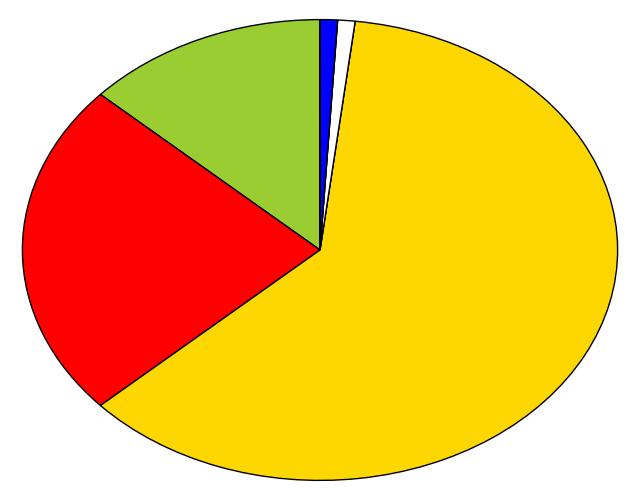
\includegraphics[width=\textwidth]{arousalALLpearsonR}
    \caption{Pearson correlation}
  \end{subfigure}
  \hfill
  \begin{subfigure}[b]{0.3\textwidth}
    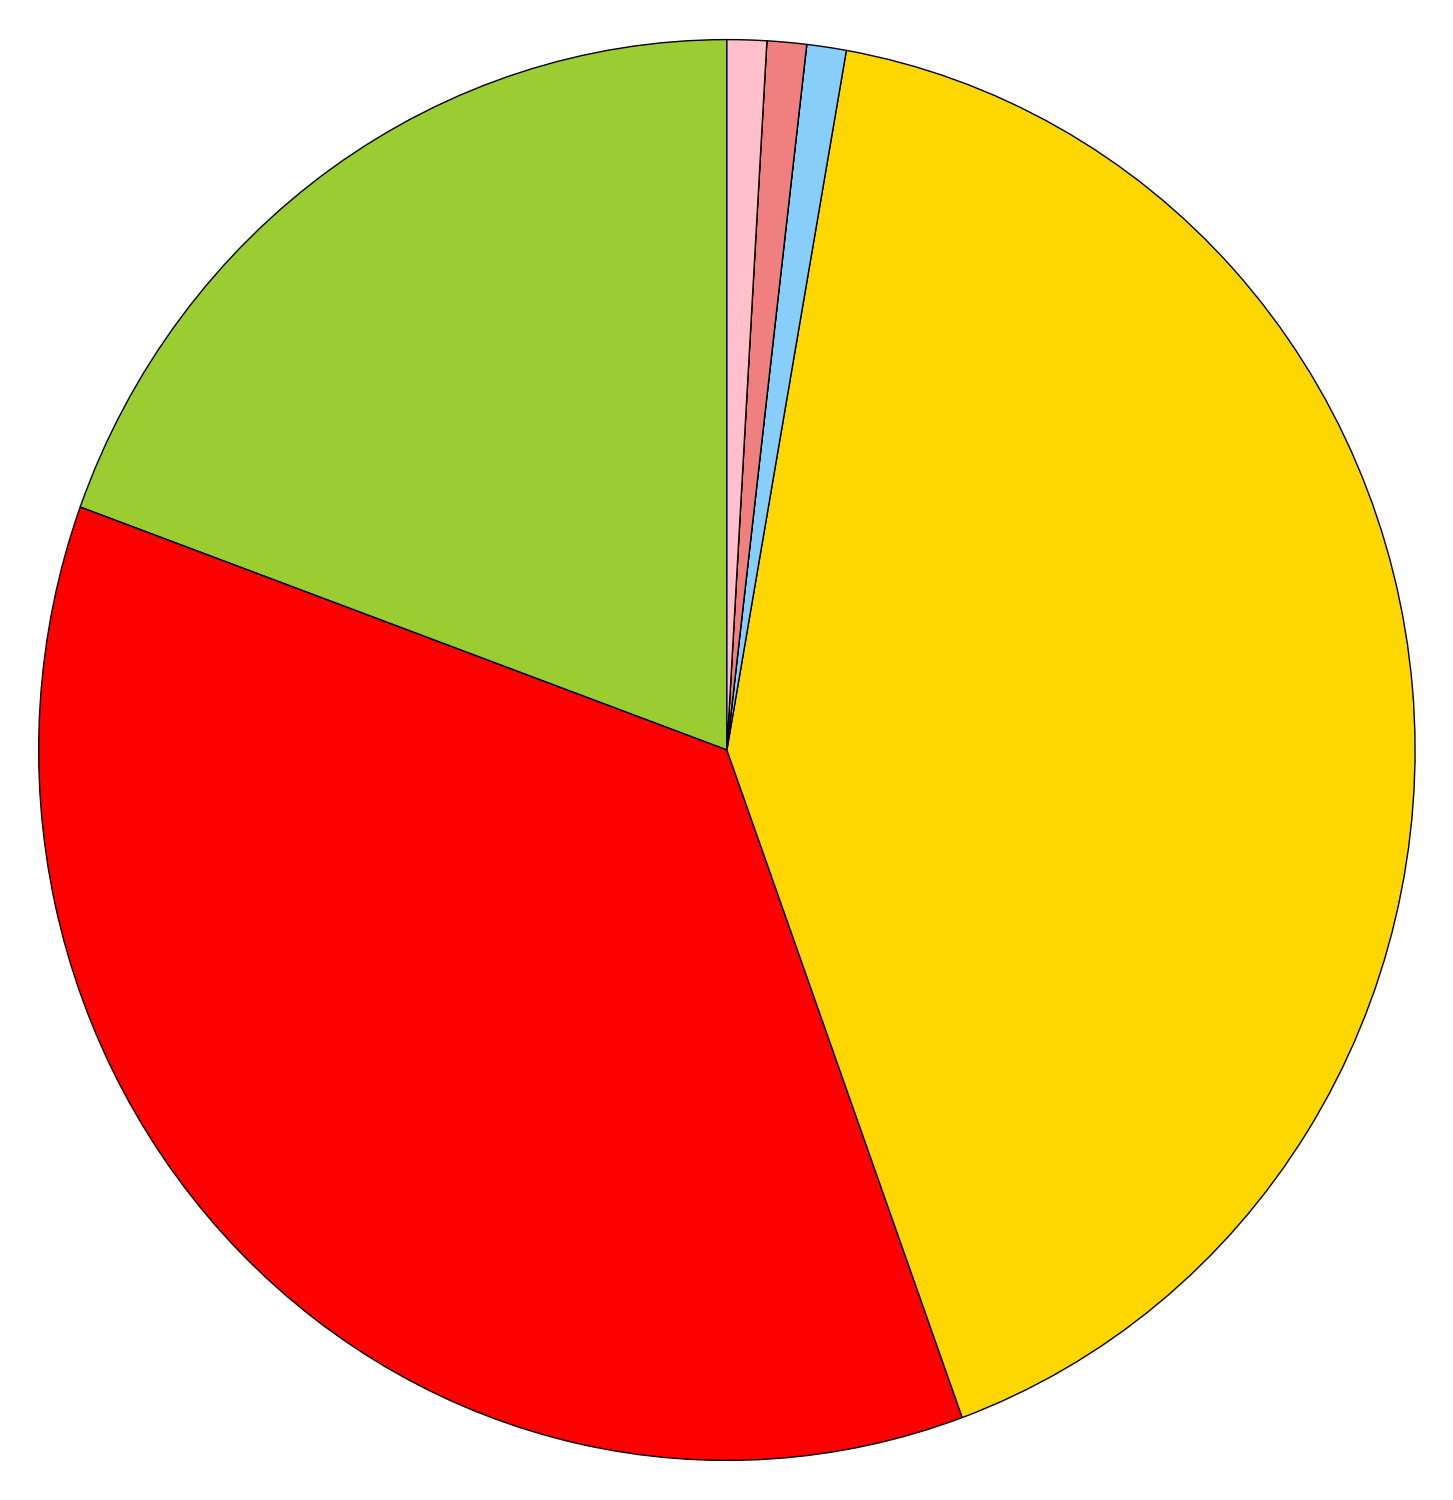
\includegraphics[width=\textwidth]{arousalALLMutInf}
    \caption{Mutual information}
  \end{subfigure}
  \hfill
  \begin{subfigure}[b]{0.3\textwidth}
    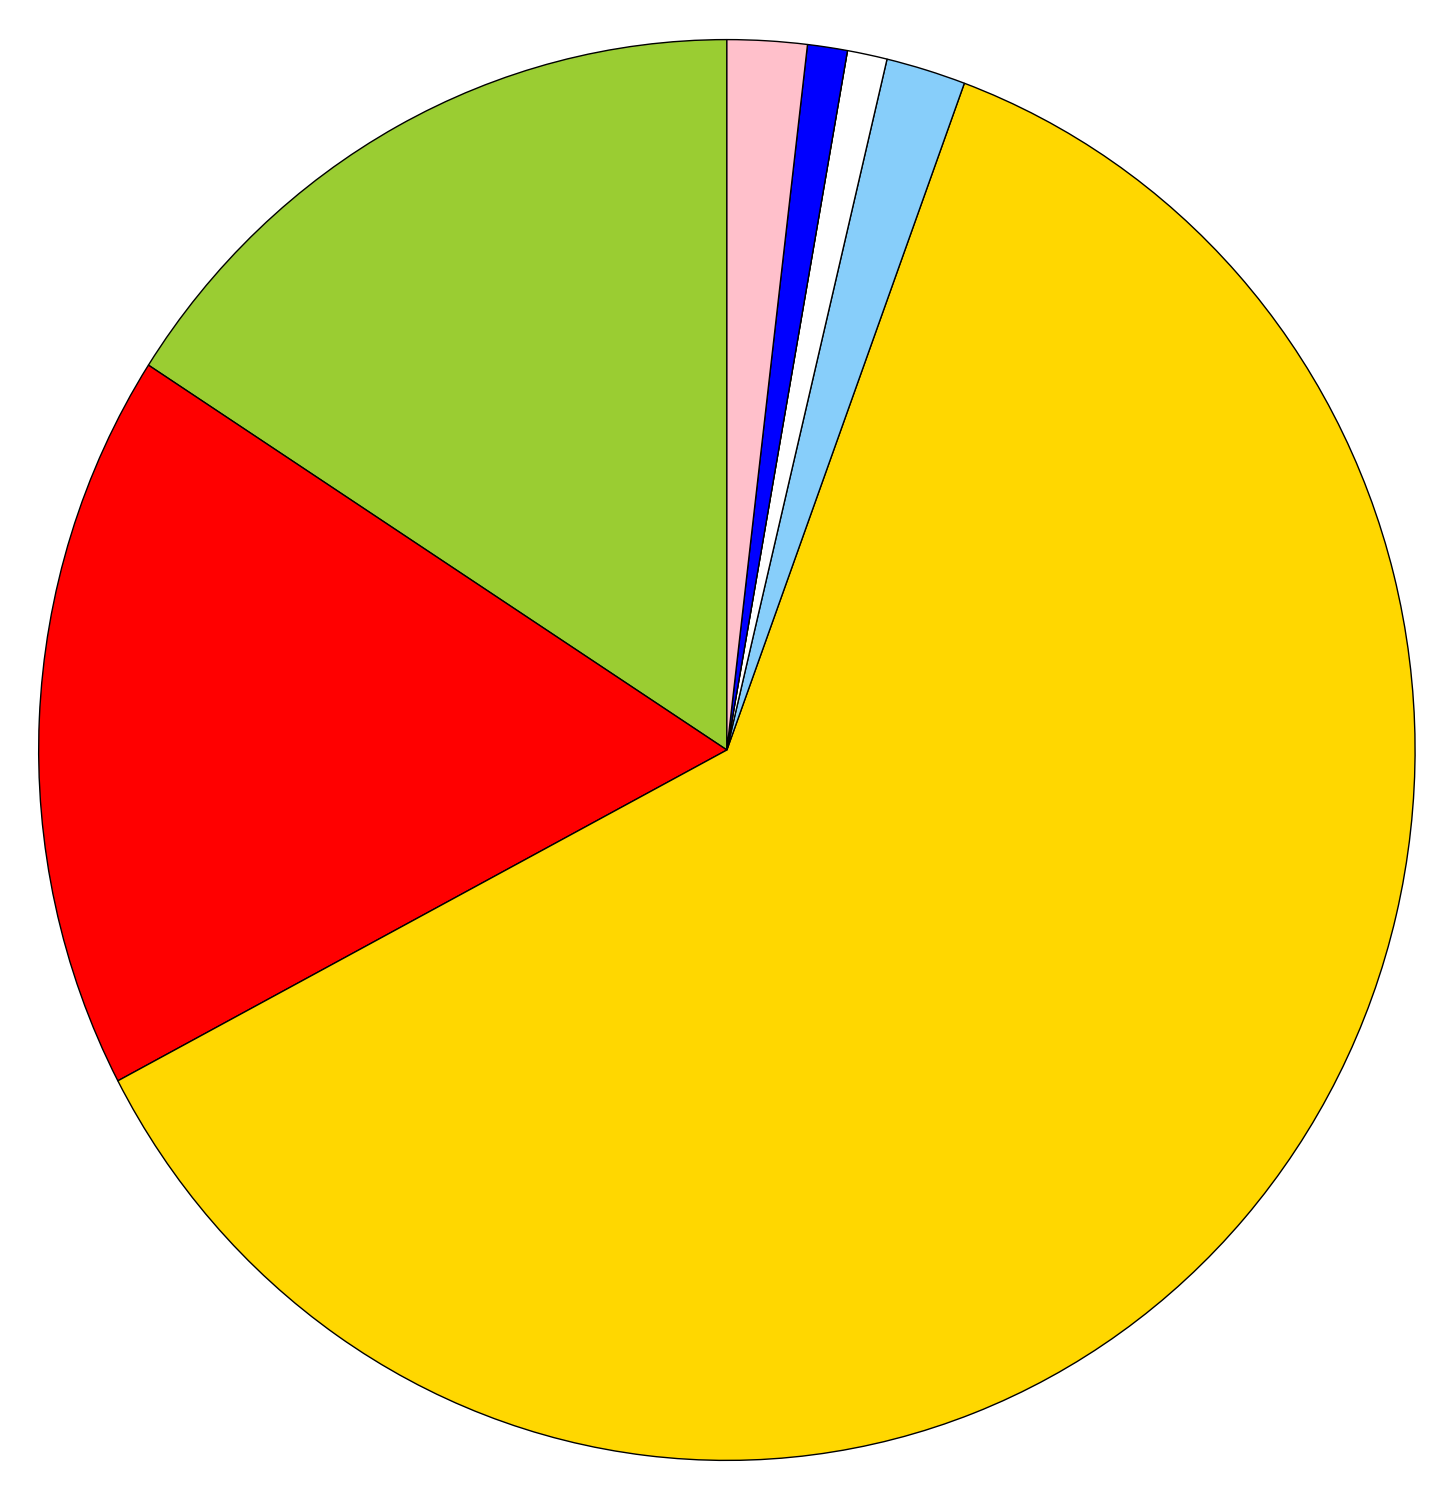
\includegraphics[width=\textwidth]{arousalALLdCorr}
    \caption{Distance Correlation}
  \end{subfigure}
  
  \begin{subfigure}[b]{0.3\textwidth}
    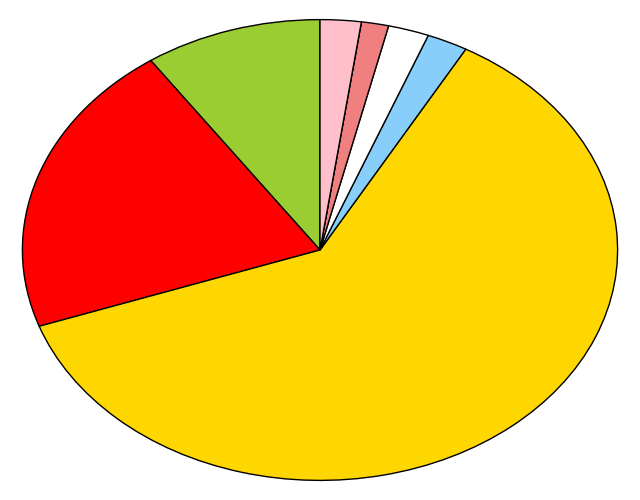
\includegraphics[width=\textwidth]{arousalALLANOVA}
    \caption{ANOVA}
  \end{subfigure}
  \hfill
  \begin{subfigure}[b]{0.3\textwidth}
    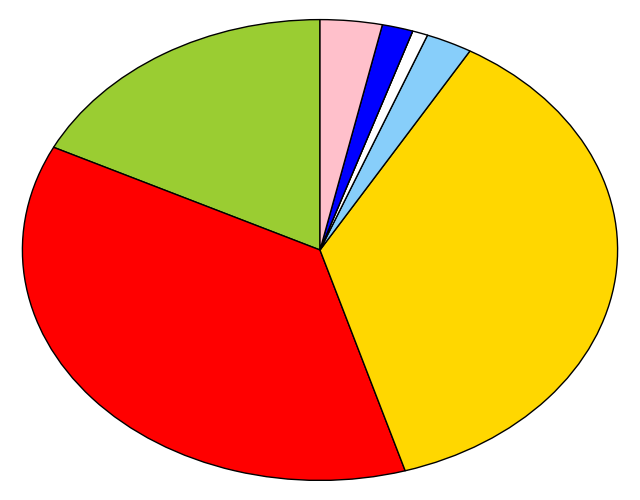
\includegraphics[width=\textwidth]{arousalALLLR}
    \caption{Linear regression}
  \end{subfigure}
  \hfill
  \begin{subfigure}[b]{0.3\textwidth}
    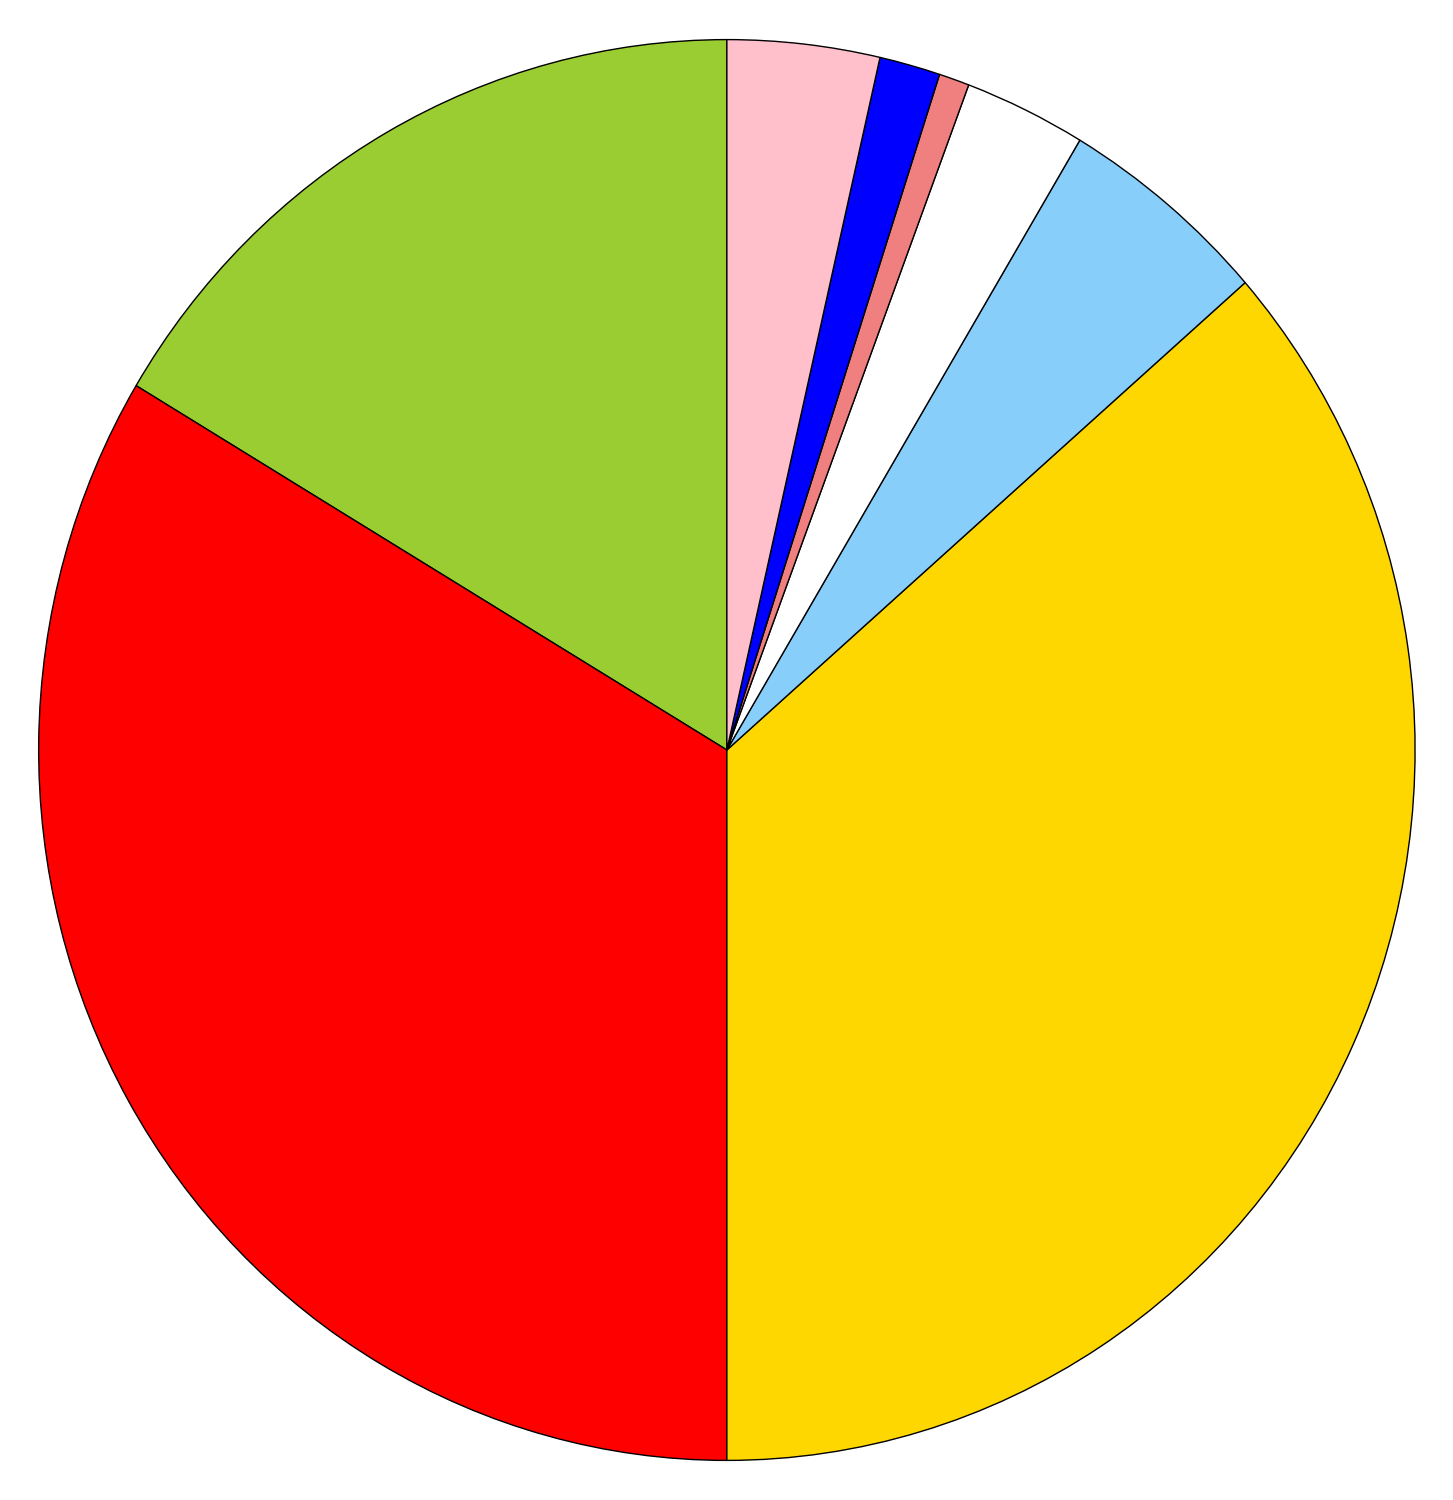
\includegraphics[width=\textwidth]{arousalALLSVM}
    \caption{SVM}
  \end{subfigure}
  
  \begin{subfigure}[b]{0.3\textwidth}
    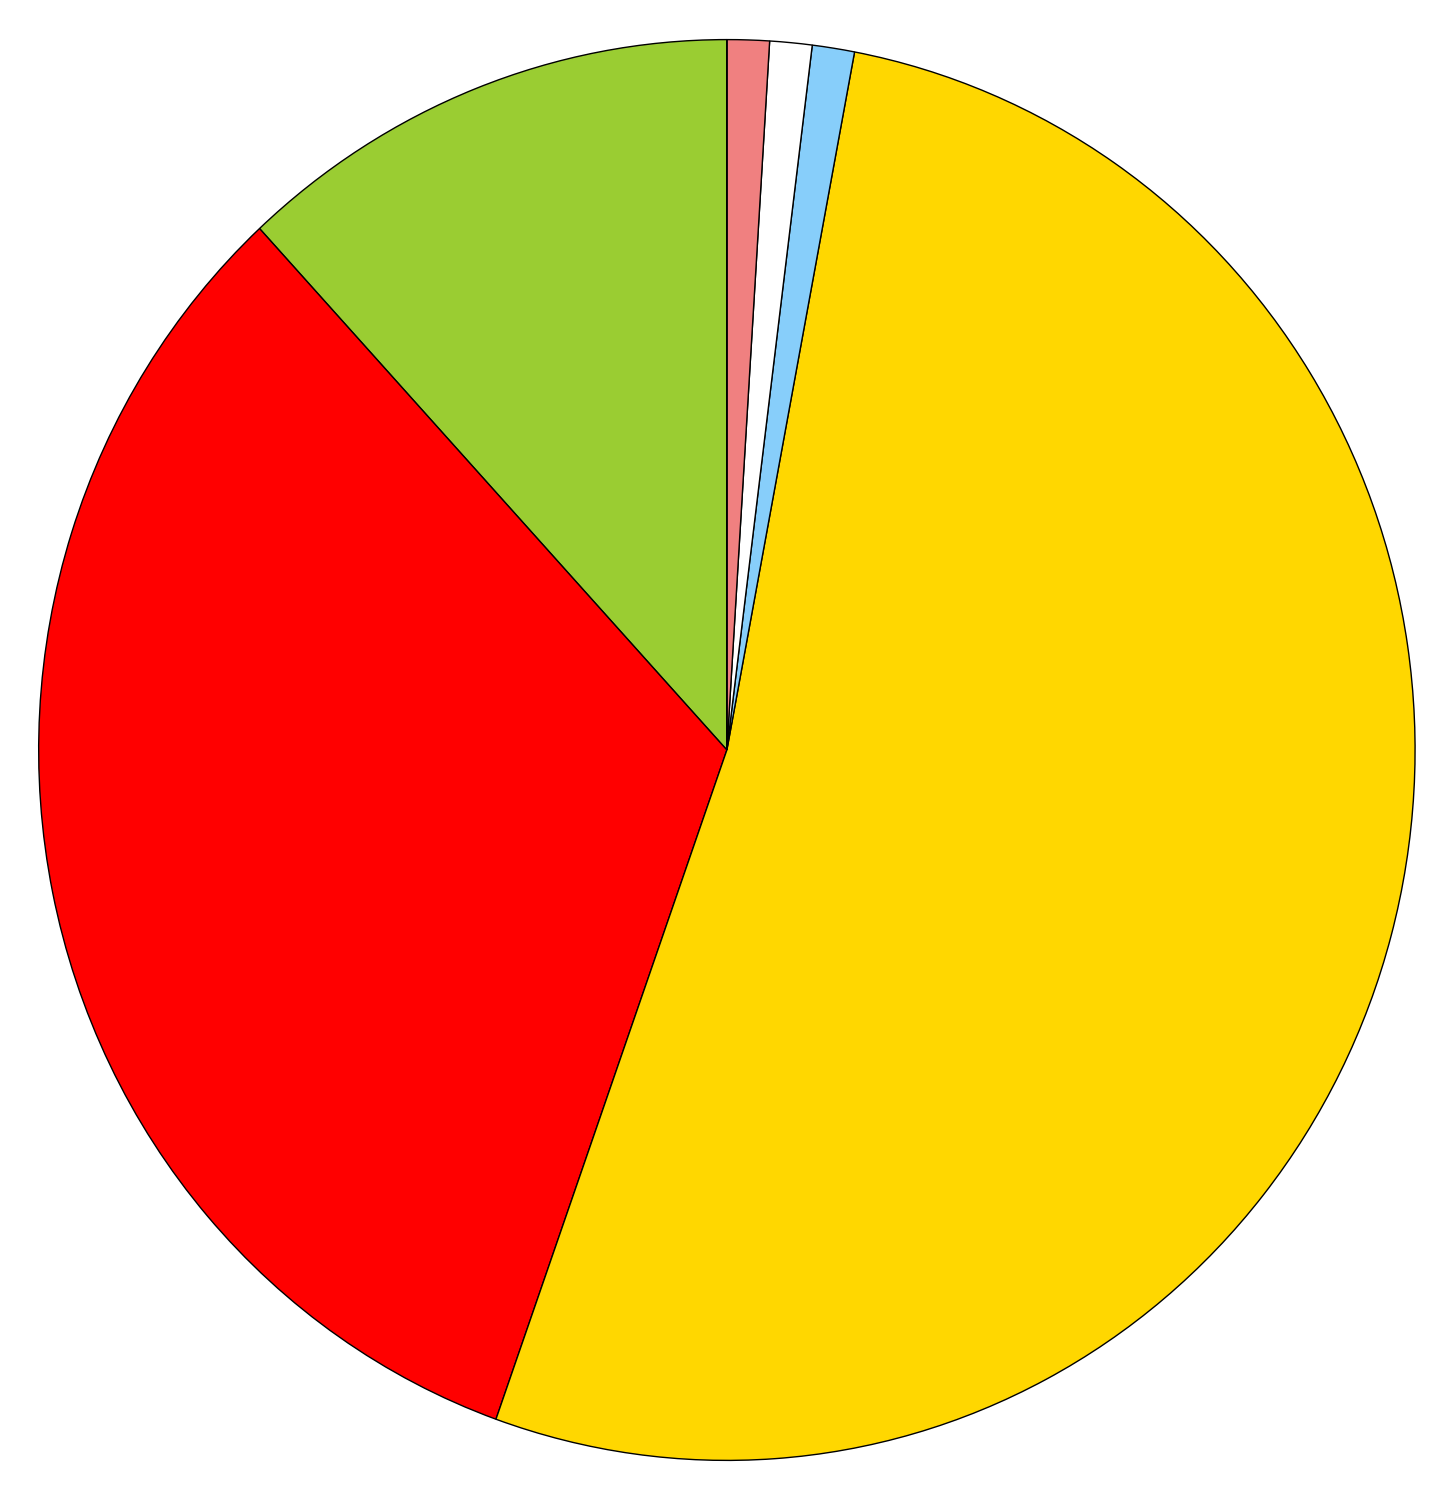
\includegraphics[width=\textwidth]{arousalALLLDA}
    \caption{LDA}
  \end{subfigure}
  \hfill
  \begin{subfigure}[b]{0.3\textwidth}
    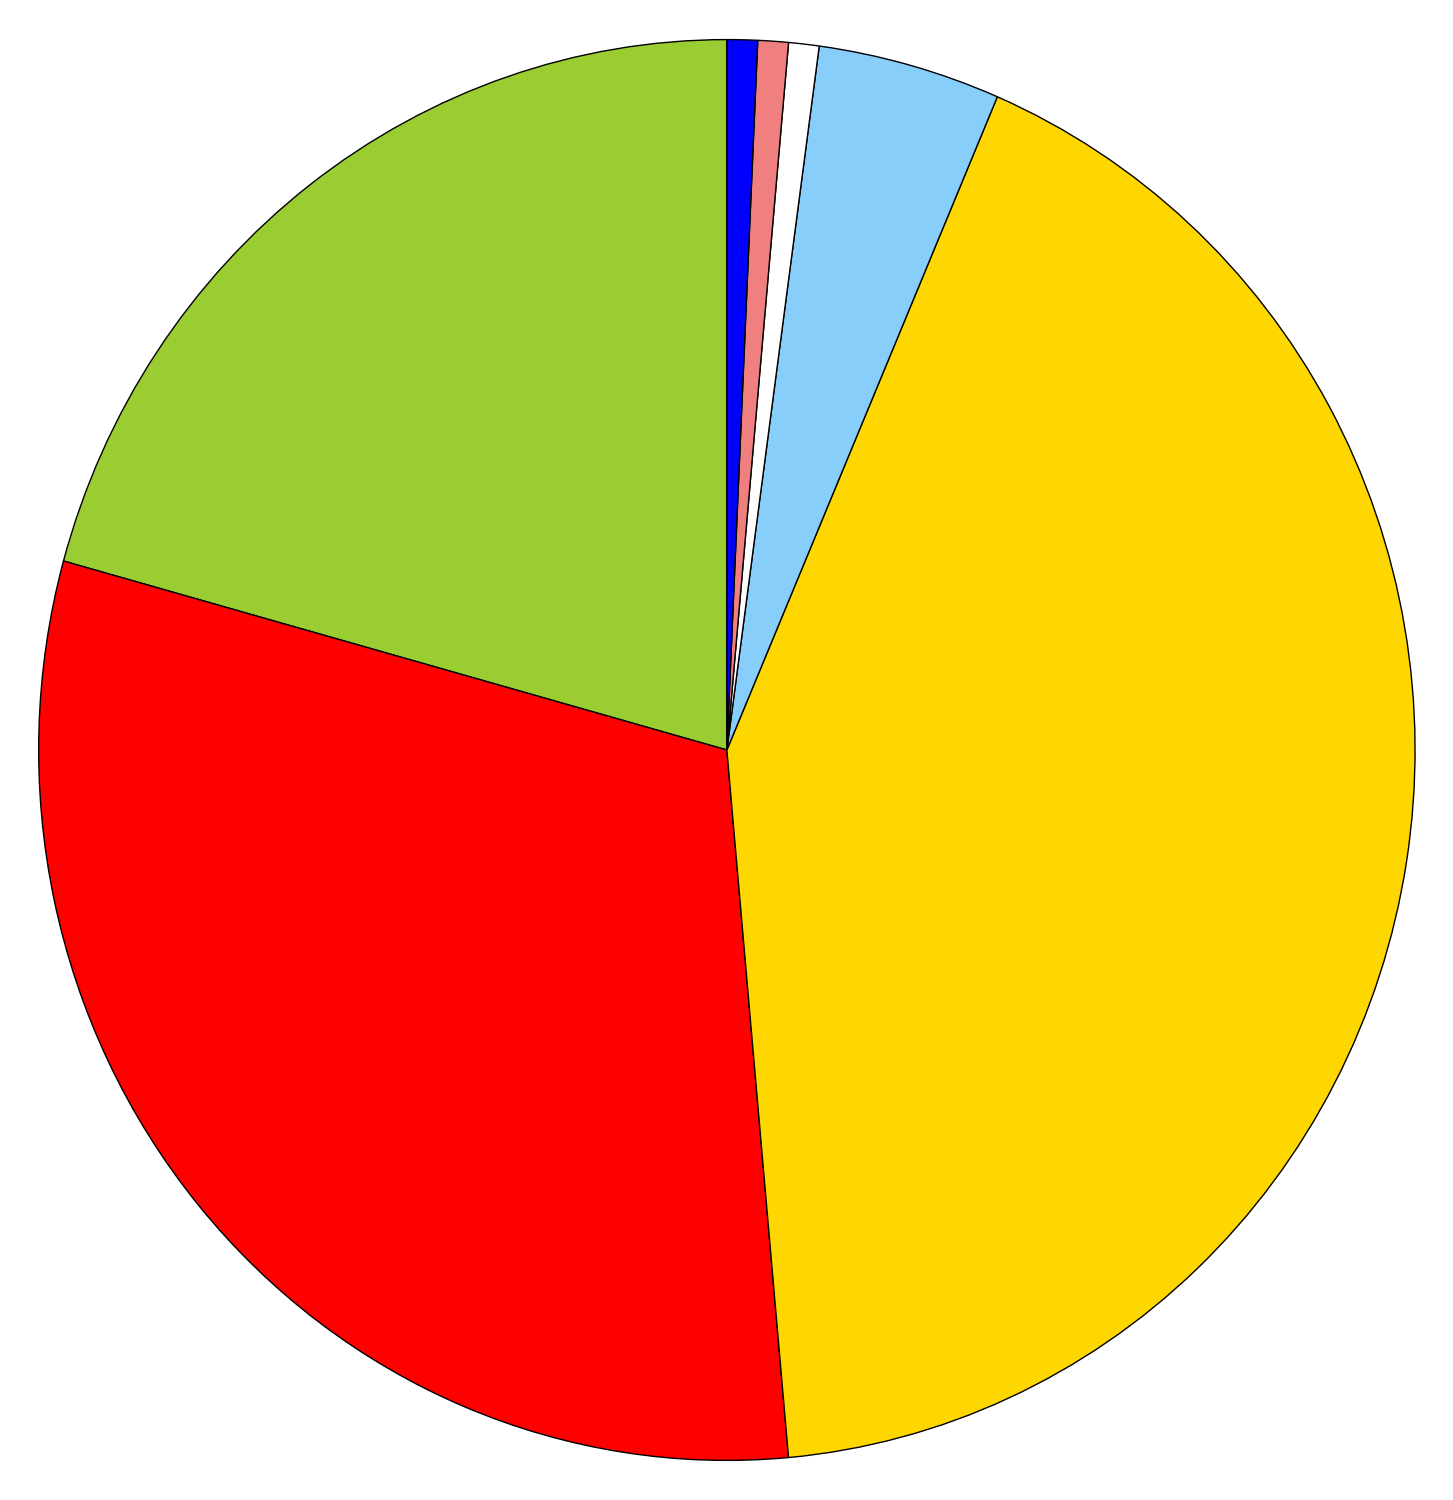
\includegraphics[width=\textwidth]{arousalALLL1}
    \caption{Lasso regression}
  \end{subfigure}
  \hfill
  \begin{subfigure}[b]{0.3\textwidth}
    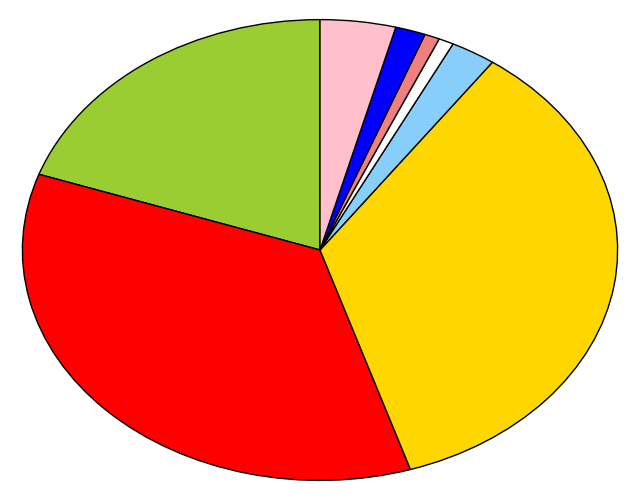
\includegraphics[width=\textwidth]{arousalALLL2}
    \caption{Ridge regression}
  \end{subfigure}
  
  \begin{subfigure}[b]{0.3\textwidth}
    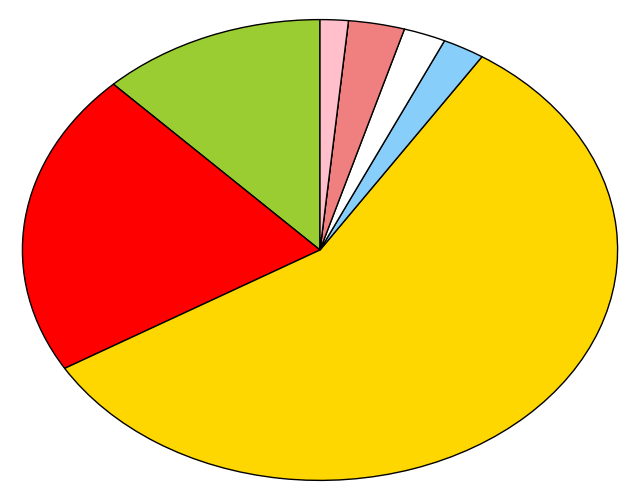
\includegraphics[width=\textwidth]{arousalALLRF}
    \caption{Random forests}
  \end{subfigure}
  \hfill
  \begin{subfigure}[b]{0.3\textwidth}
    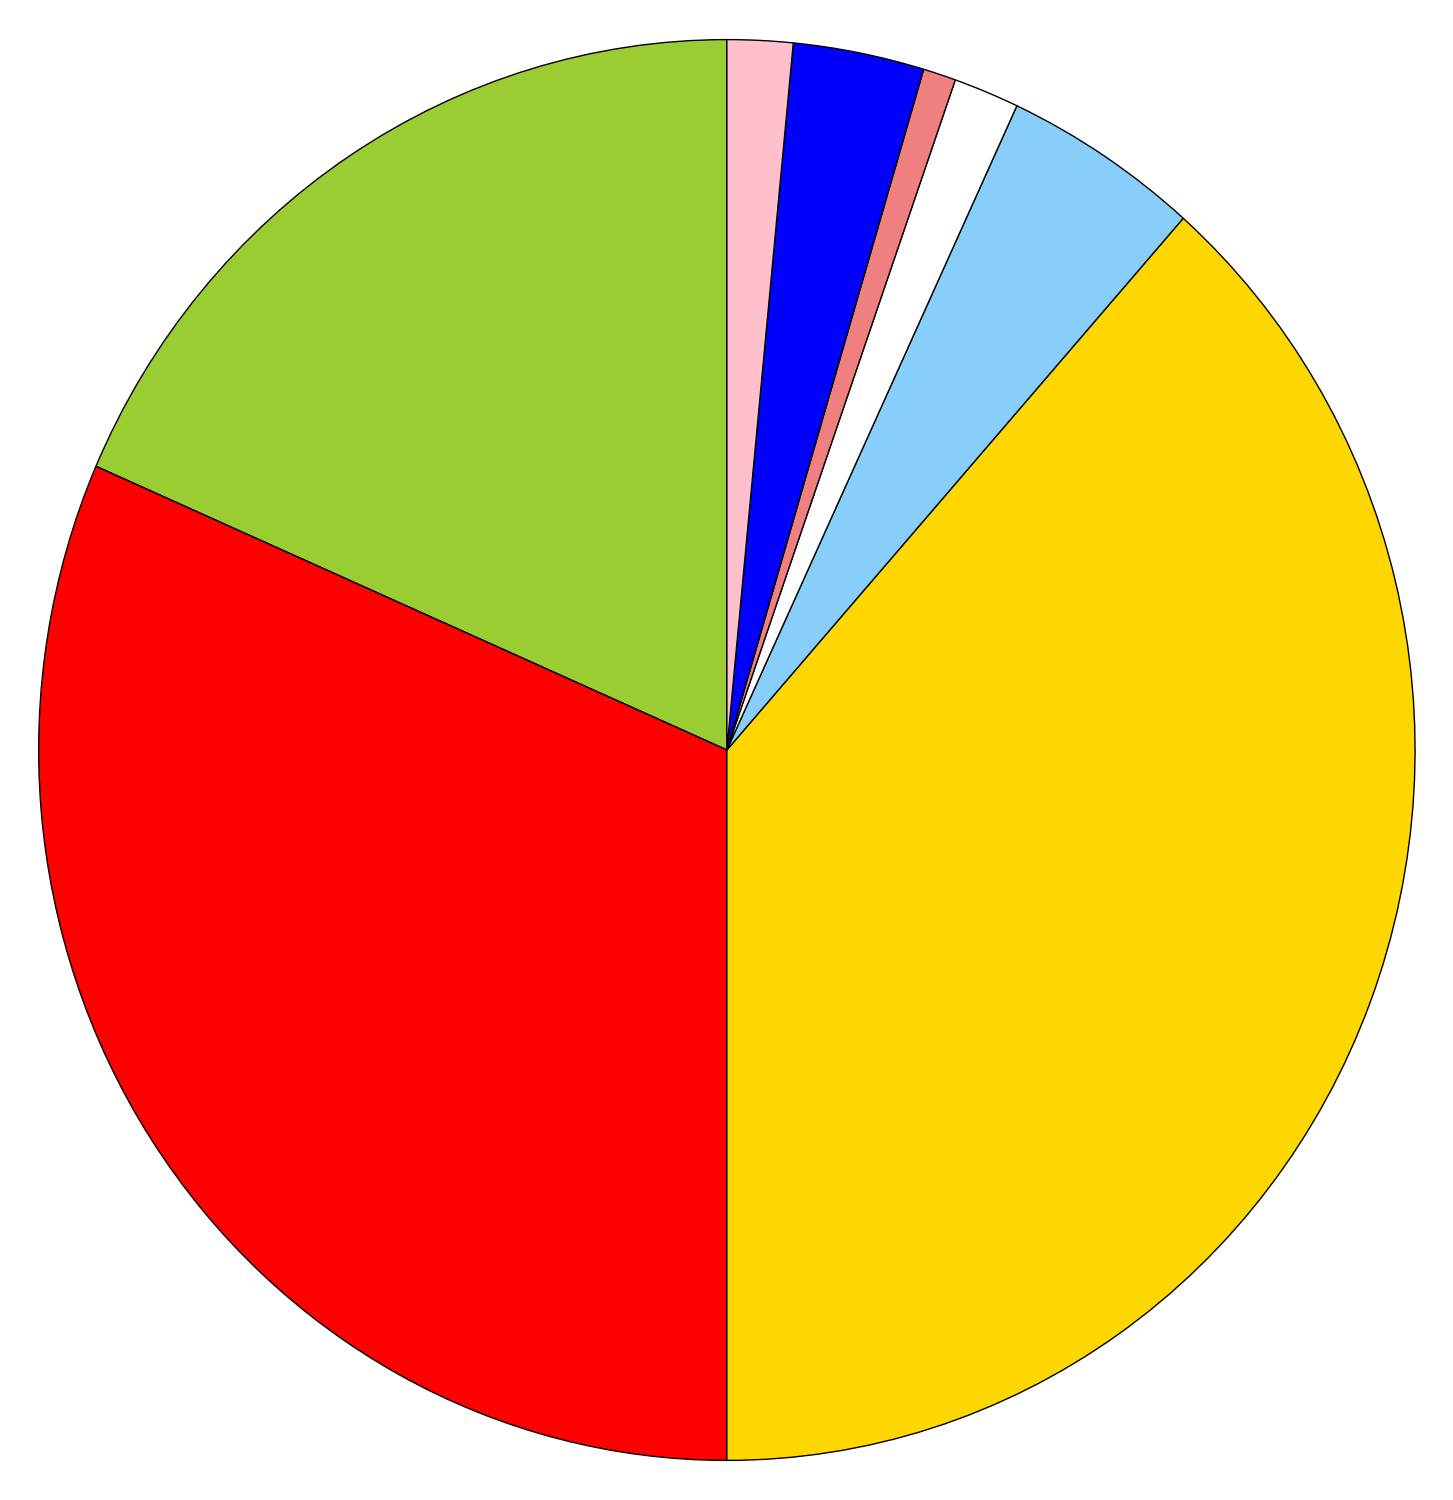
\includegraphics[width=\textwidth]{arousalALLPCA}
    \caption{PCA}
  \end{subfigure}
  \hfill
  \begin{subfigure}[b]{0.3\textwidth}
    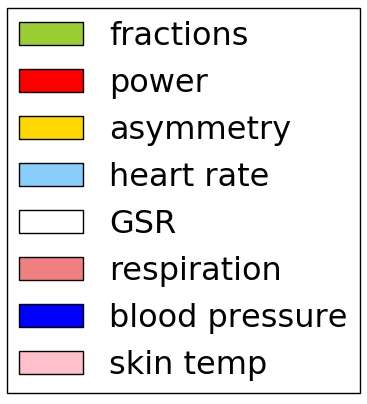
\includegraphics[width=\textwidth]{legend}
    \caption{Legend\label{arousalpieslegend}}
  \end{subfigure}
\end{figure}

\clearpage

\begin{figure}[!tbp]
  \centering
  \caption{Selection features for valence classification.\label{valencepies}}
  \begin{subfigure}[b]{0.3\textwidth}
    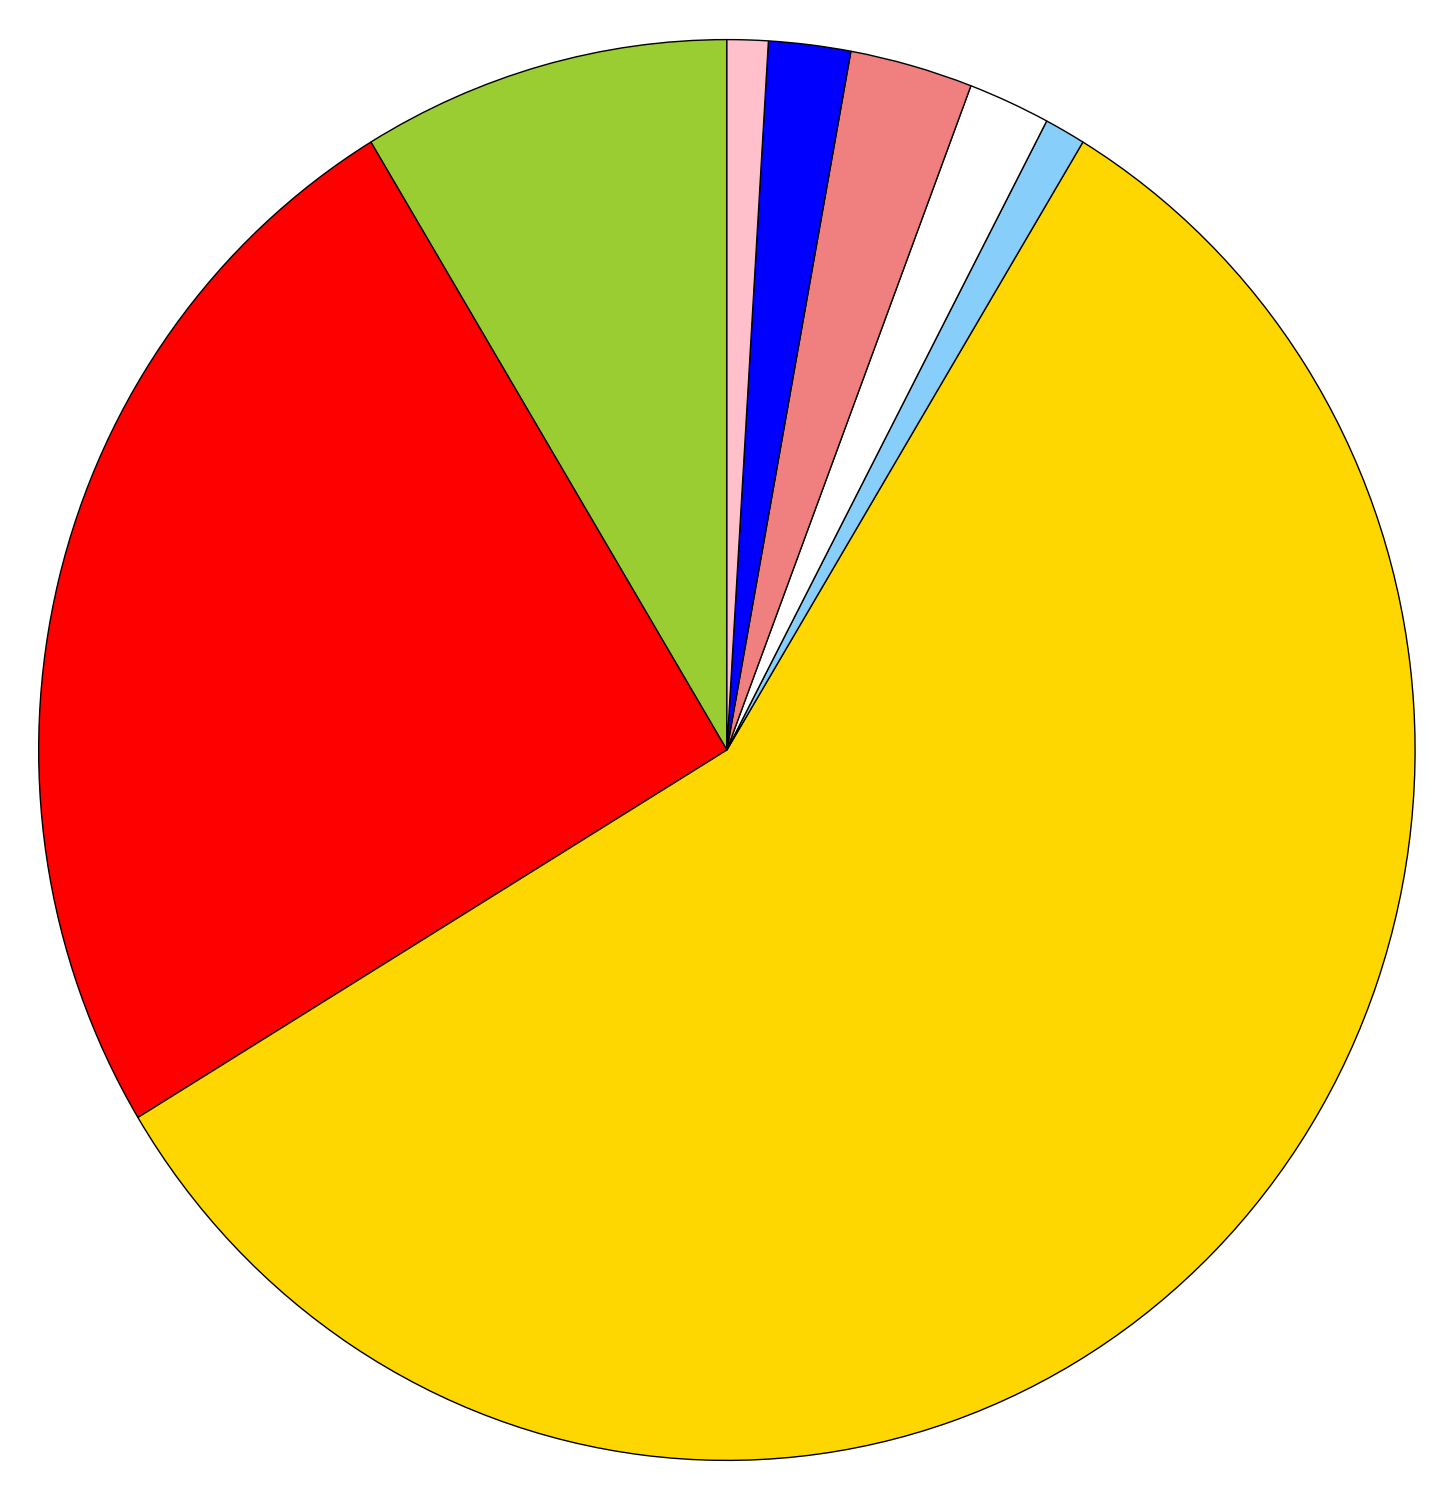
\includegraphics[width=\textwidth]{valenceALLpearsonR}
    \caption{Pearson correlation}
  \end{subfigure}
  \hfill
  \begin{subfigure}[b]{0.3\textwidth}
    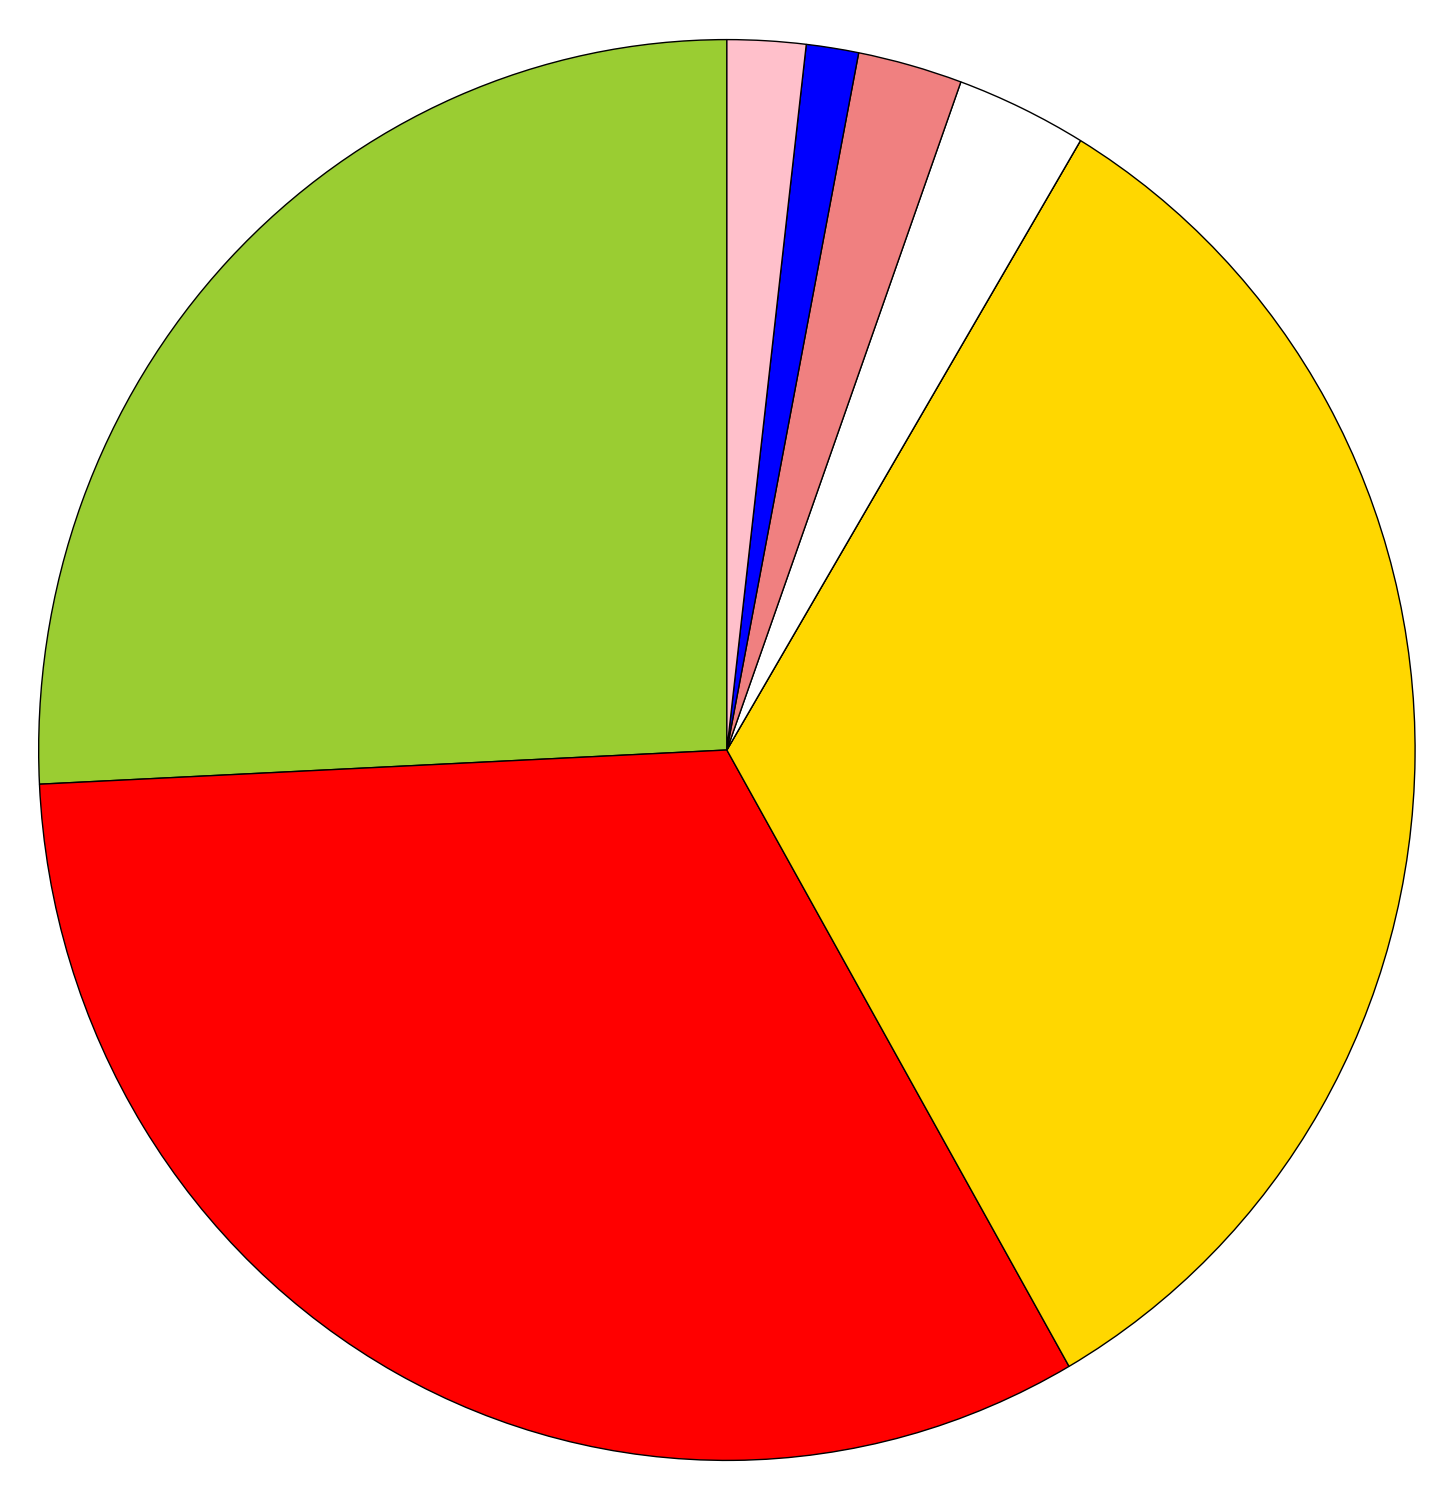
\includegraphics[width=\textwidth]{valenceALLMutInf}
    \caption{Mutual information}
  \end{subfigure}
  \hfill
  \begin{subfigure}[b]{0.3\textwidth}
    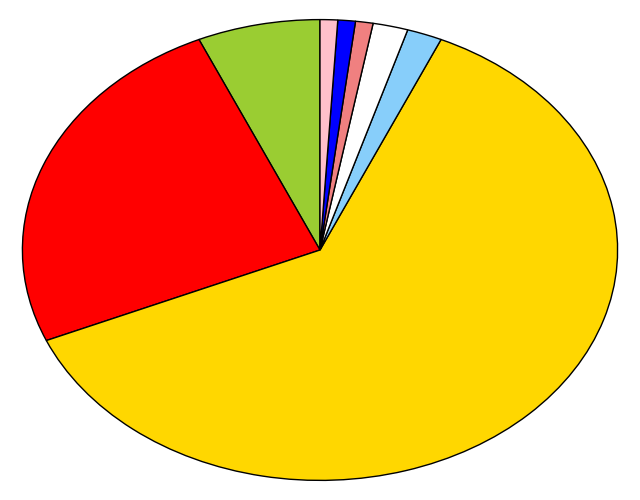
\includegraphics[width=\textwidth]{valenceALLdCorr}
    \caption{Distance Correlation}
  \end{subfigure}
  
  \begin{subfigure}[b]{0.3\textwidth}
    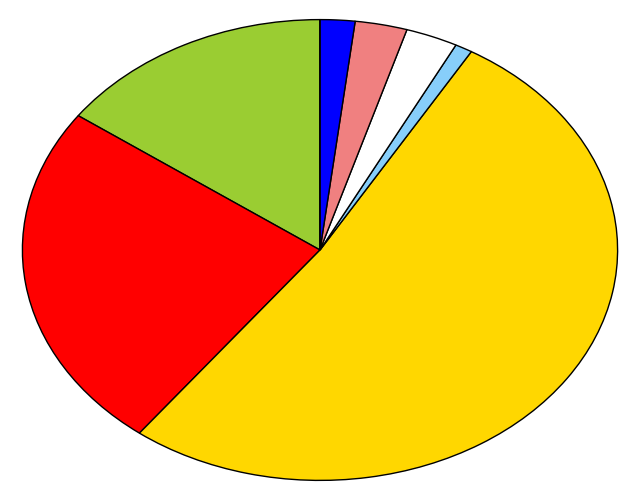
\includegraphics[width=\textwidth]{valenceALLANOVA}
    \caption{ANOVA}
  \end{subfigure}
  \hfill
  \begin{subfigure}[b]{0.3\textwidth}
    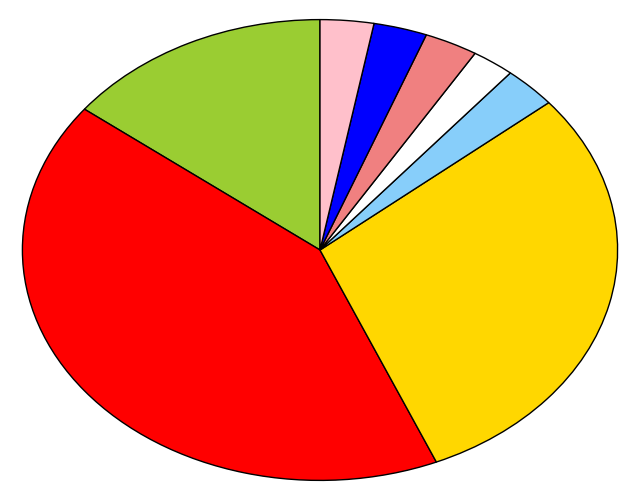
\includegraphics[width=\textwidth]{valenceALLLR}
    \caption{Linear regression}
  \end{subfigure}
  \hfill
  \begin{subfigure}[b]{0.3\textwidth}
    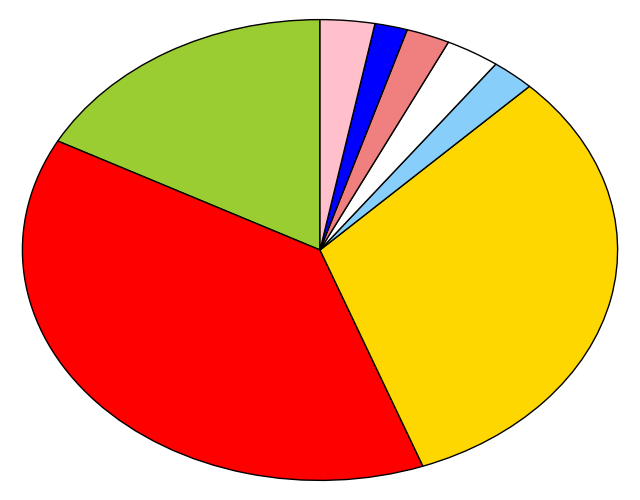
\includegraphics[width=\textwidth]{valenceALLSVM}
    \caption{SVM}
  \end{subfigure}
  
  \begin{subfigure}[b]{0.3\textwidth}
    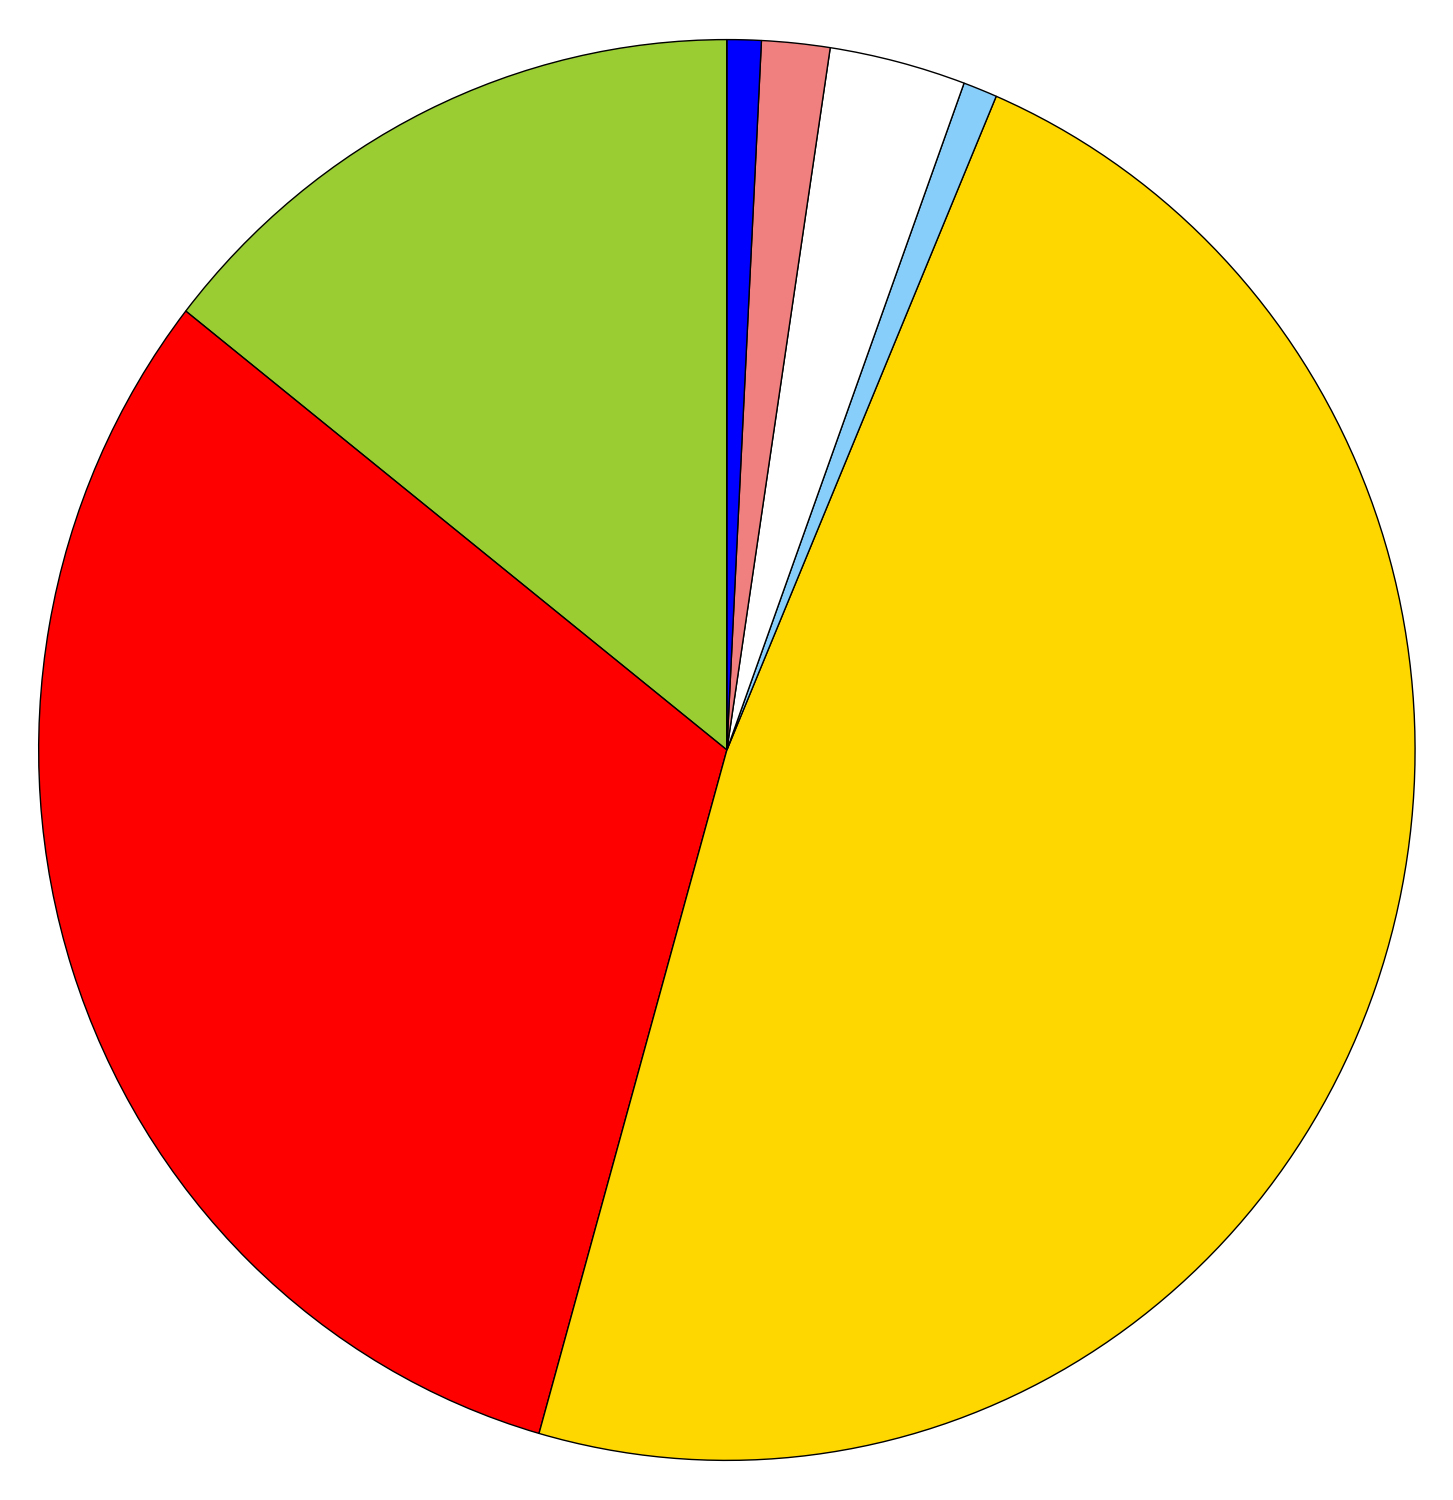
\includegraphics[width=\textwidth]{valenceALLLDA}
    \caption{LDA}
  \end{subfigure}
  \hfill
  \begin{subfigure}[b]{0.3\textwidth}
    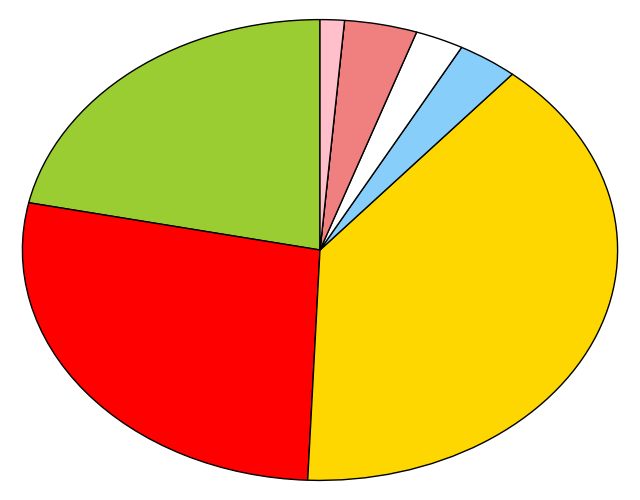
\includegraphics[width=\textwidth]{valenceALLL1}
    \caption{Lasso regression}
  \end{subfigure}
  \hfill
  \begin{subfigure}[b]{0.3\textwidth}
    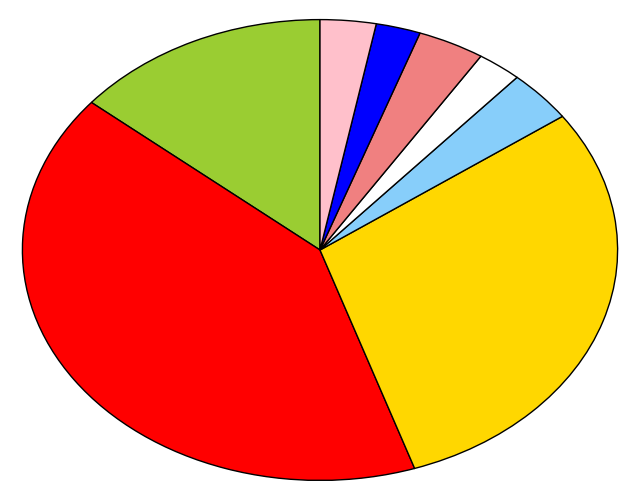
\includegraphics[width=\textwidth]{valenceALLL2}
    \caption{Ridge regression}
  \end{subfigure}
  
  \begin{subfigure}[b]{0.3\textwidth}
    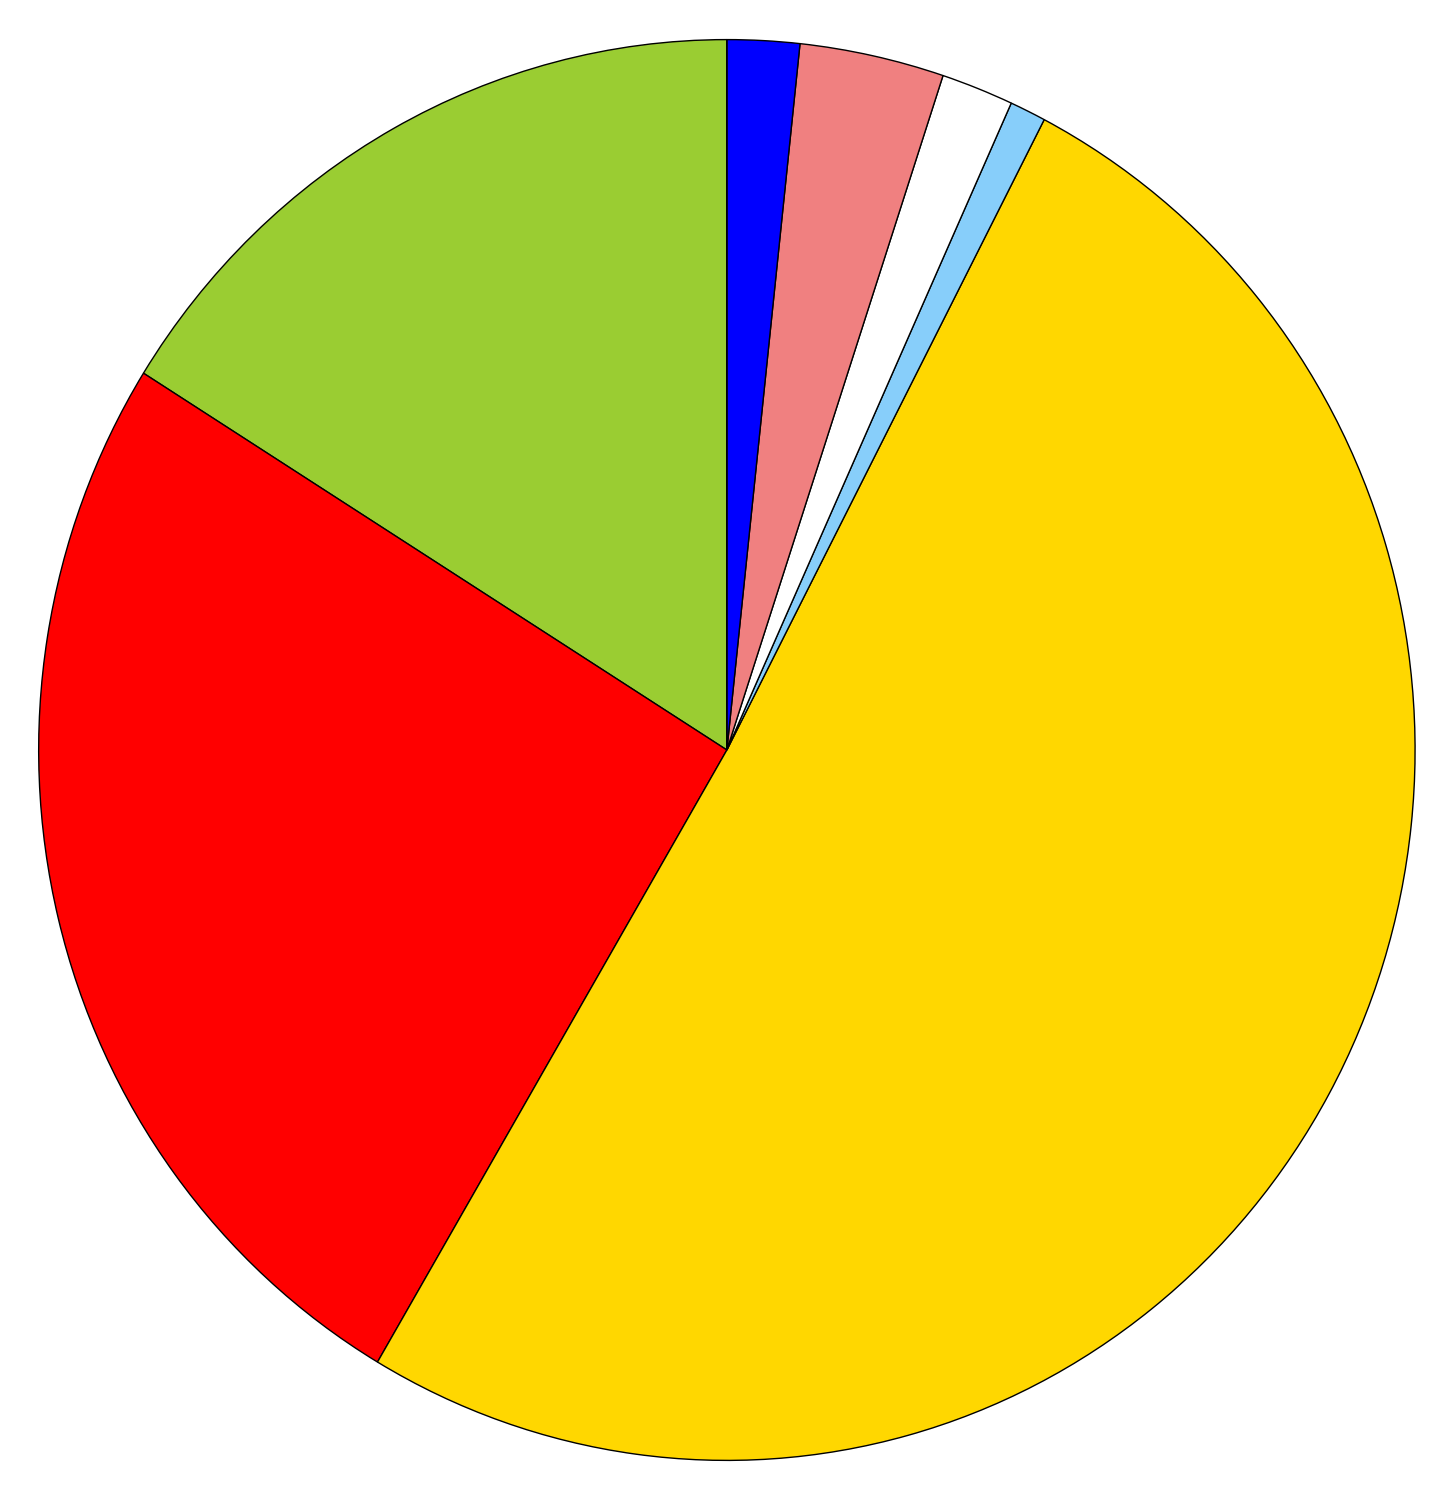
\includegraphics[width=\textwidth]{valenceALLRF}
    \caption{Random forests}
  \end{subfigure}
  \hfill
  \begin{subfigure}[b]{0.3\textwidth}
    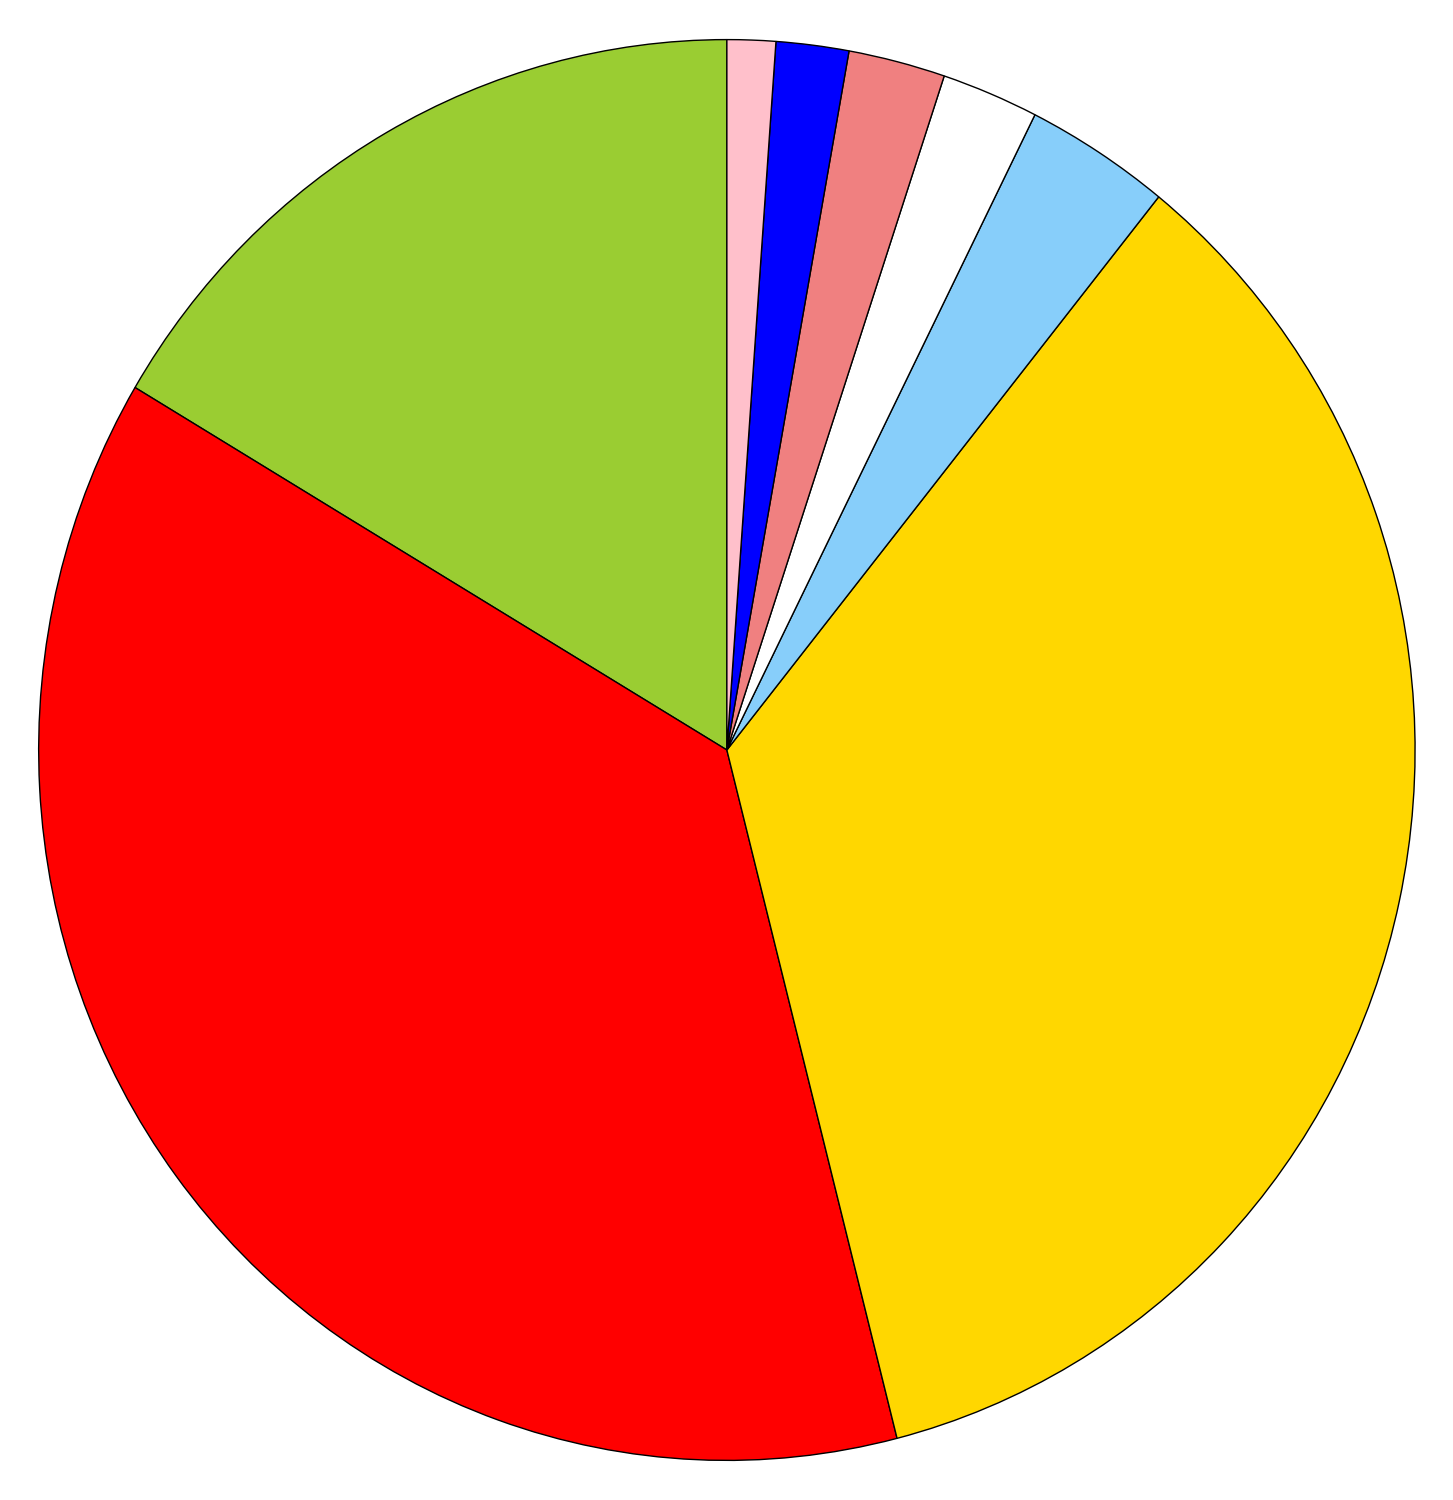
\includegraphics[width=\textwidth]{valenceALLPCA}
    \caption{PCA}
  \end{subfigure}
  \hfill
  \begin{subfigure}[b]{0.3\textwidth}
    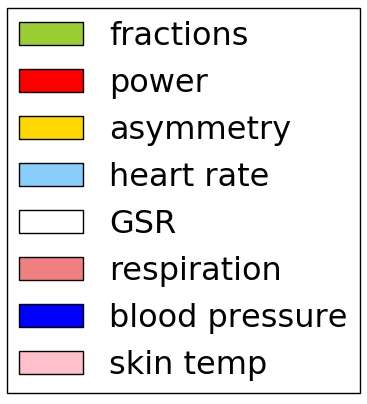
\includegraphics[width=\textwidth]{legend}
    \caption{Legend\label{valencepieslegend}}
  \end{subfigure}
\end{figure}
\clearpage

The fact that the non-EEG features are almost never chosen might indicate that they are less important. In an attempt to further investigate the difference between EEG features and non-EEG features, the performance of three different feature sets was compared. The first feature set is the previously used feature set with all possible features. The second and third feature sets contained only EEG and non-EEG features respectively. The feature selection was done with random forest, as this method had the best average performance, as well as the best correlations between probability and level of valence and arousal. 

\npar

The resulting performances of these different features sets are displayed in Figure \ref{arousalphyeegall} for arousal and in Figure \ref{valencephyeegall} for valence. The exact values are shown in Table \ref{phyeegalltable}.

\mijnfiguur{width=1.\textwidth}{arousalphyeegall}{The performance of arousal prediction for all, EEG and non-EEG features.}

\mijnfiguur{width=1.\textwidth}{valencephyeegall}{The performance of valence prediction for all, EEG and non-EEG features.}

\begin{table}[H]
\centering
\begin{tabular}{l|ll|ll}
         & \textbf{Arousal} &         & \textbf{Valence} &         \\
\textbf{Feat set} & \textbf{avg acc} & \textbf{std acc} & \textbf{avg acc} & \textbf{std acc} \\ \hline 
\textbf{all}      & 0.7000  & 0.1369  & 0.7375  & 0.1293  \\
\textbf{EEG}      & 0.7188  & 0.1310  & 0.7281  & 0.1179  \\
\textbf{non-EEG}  & 0.6031  & 0.1425  & 0.6031  & 0.1591 
\end{tabular}
\caption{The average and standard deviation of the test accuracies (over the different persons) for the different feature sets, using the random forest feature selection model.\label{phyeegalltable}}
\end{table}

It is clear that for both valence and arousal, the average test performances are lower in case only non-EEG features are used. However the difference was not significant. The two sided p-values for each pair of features sets, are displayed in Table \ref{pvals} below:

\begin{table}[H]
\centering
\begin{tabular}{l|lll}
	    & \textbf{all / eeg} & \textbf{all / phy} & \textbf{eeg / phy} \\ \hline
\textbf{P-value} & 0.2225             & 0.79999            & 0.7955            
\end{tabular}
\caption{P-values\label{pvals}}
\end{table}
\clearpage

Next, for each of the three feature sets, a comparison of the selected features was made. As you can see on Figure \ref{arousalEEGpies} for arousal and Figure \ref{valenceEEGpies}, displayed on the following pages, the features are again mostly asymmetry features, followed by the power features. The fraction category gives only limited insight for both valence and arousal. The EEG and ALL set have similar performances, which was expected as they both use very similar features.

\npar

The results for the non-EEG features are shown in Figure \ref{arousalnon-EEGpies} for arousal and Figure \ref{valencenon-EEGpies} for valence.
Here, no single category can be labelled as most important. This is the case for both arousal and valence. However, the feature that was selected the most as being the most important for one person was the GSR, which measures perspiration. In case of valence, the first selected features were heart rate and GSR.

\clearpage
\begin{figure}[!tbp]
  \centering
  \caption{Selection features for arousal classification, using only EEG features.\label{arousalEEGpies}}
  \begin{subfigure}[b]{0.3\textwidth}
    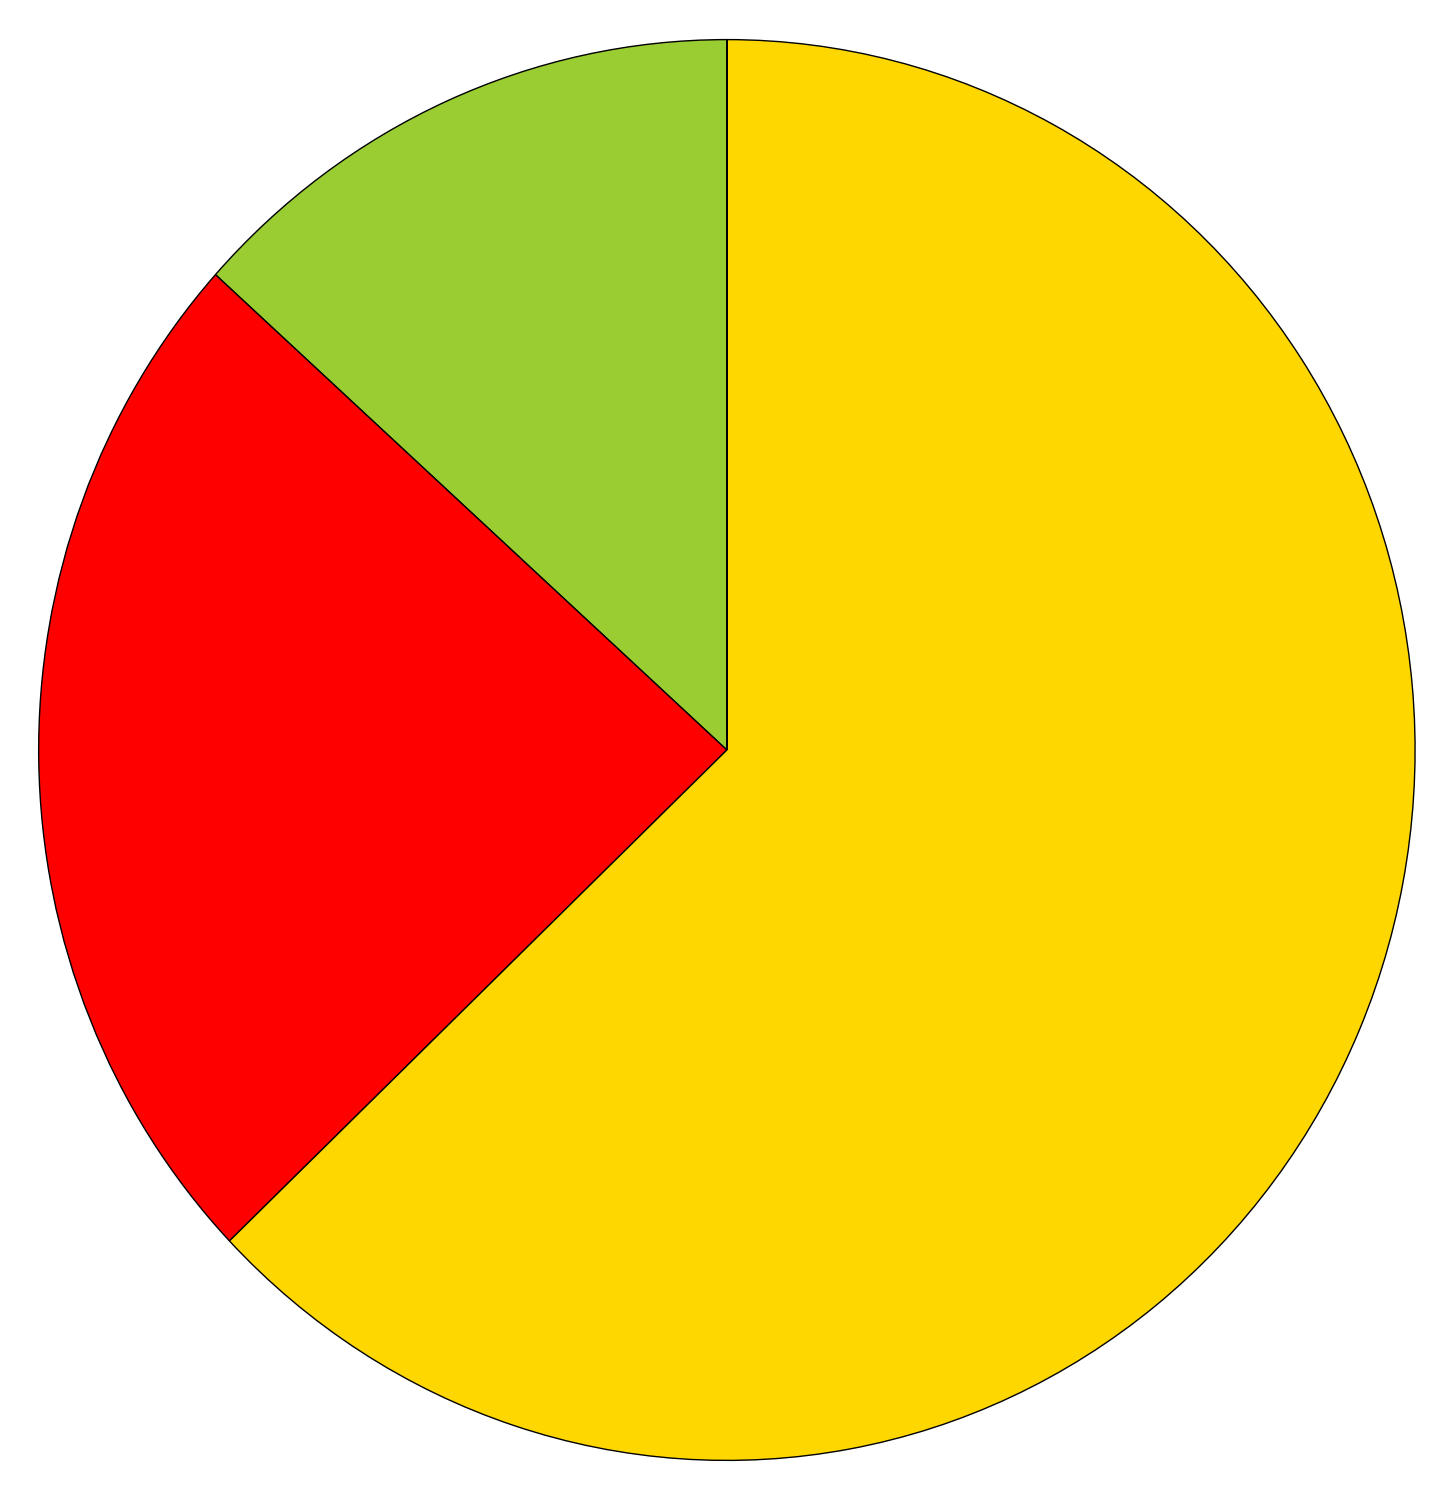
\includegraphics[width=\textwidth]{arousalEEGpearsonR}
    \caption{Pearson correlation}
  \end{subfigure}
  \hfill
  \begin{subfigure}[b]{0.3\textwidth}
    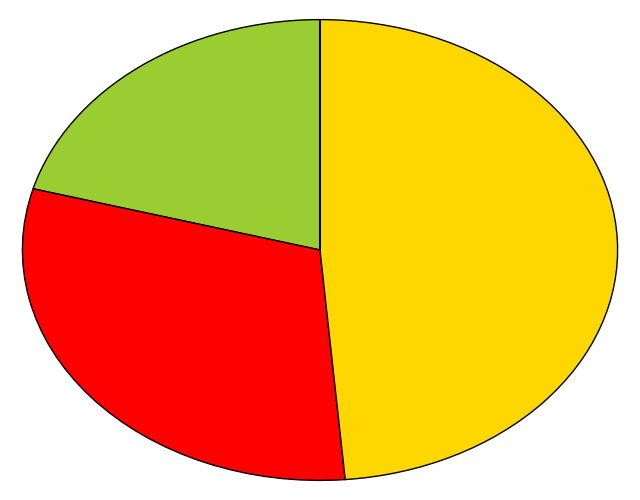
\includegraphics[width=\textwidth]{arousalEEGMutInf}
    \caption{Mutual information}
  \end{subfigure}
  \hfill
  \begin{subfigure}[b]{0.3\textwidth}
    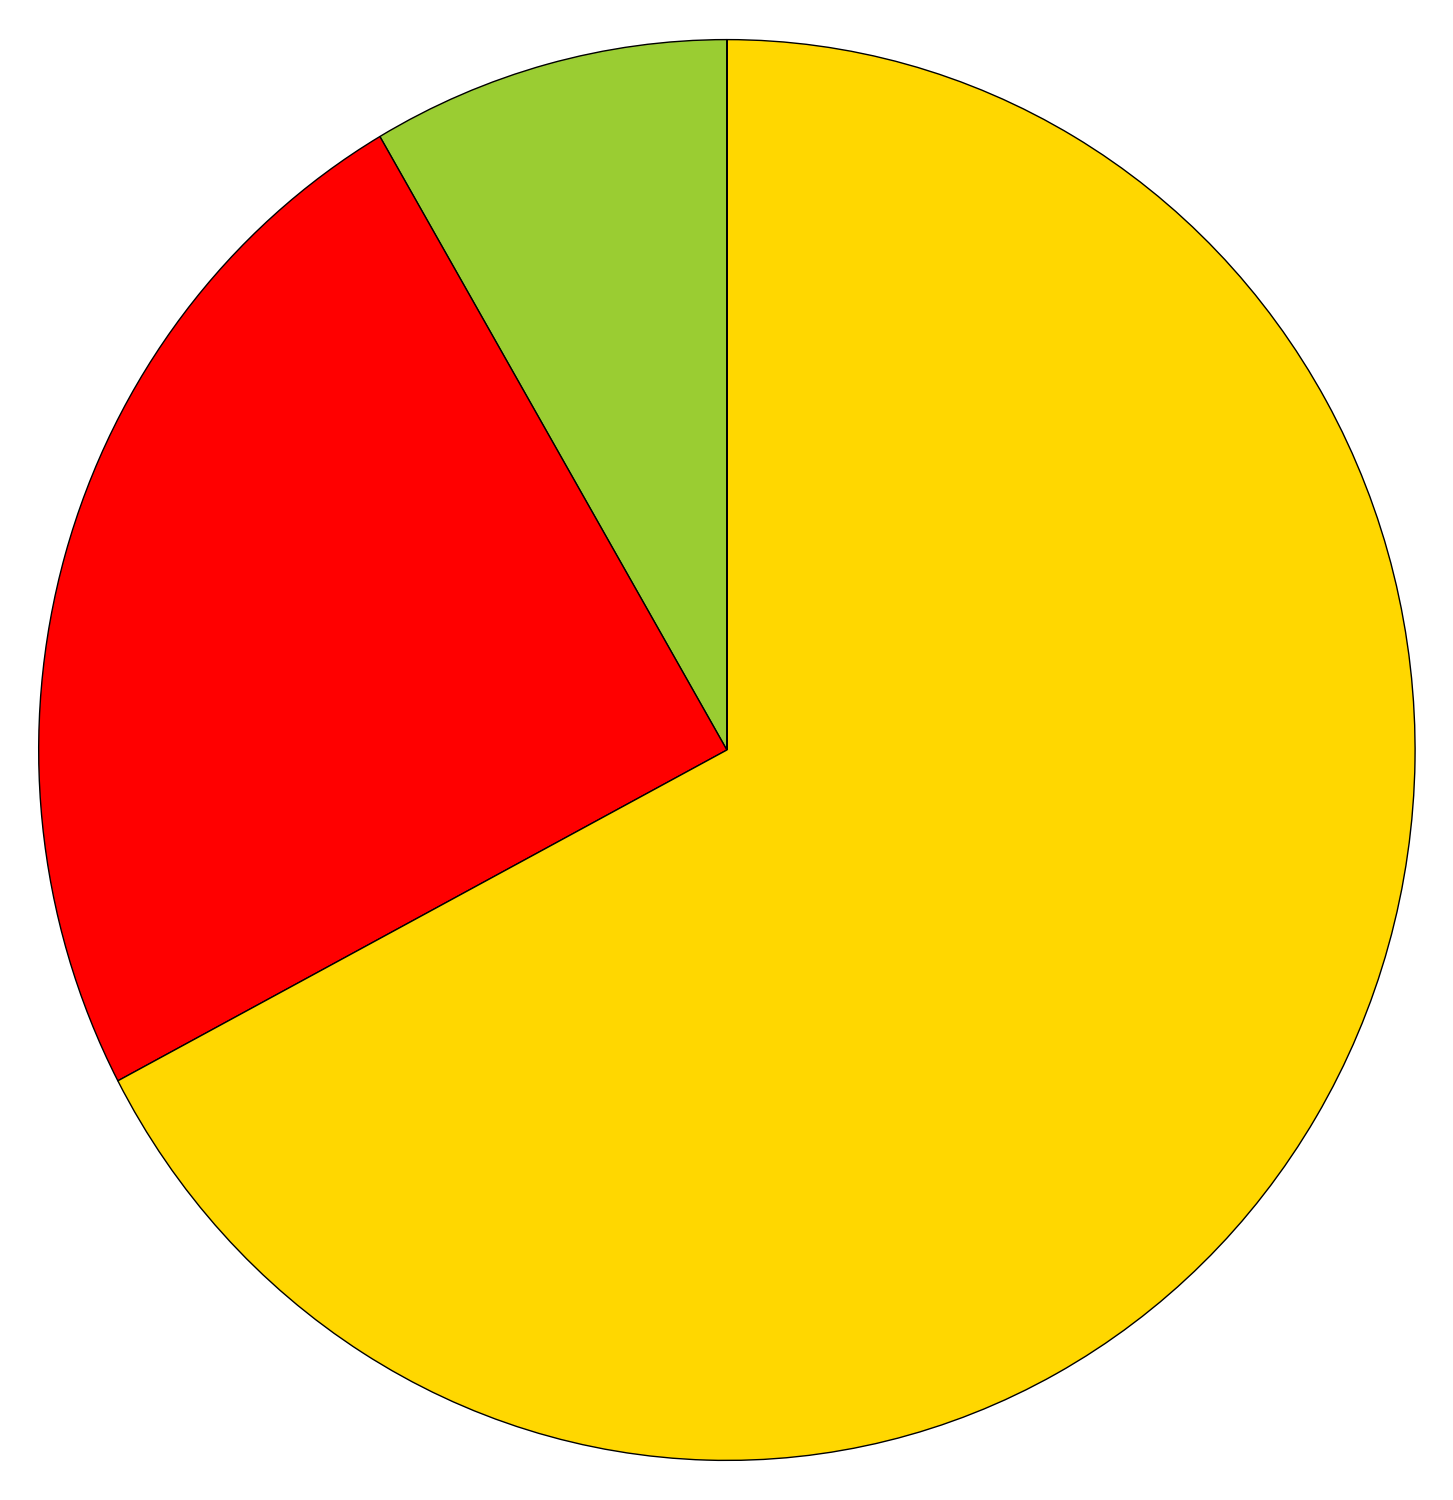
\includegraphics[width=\textwidth]{arousalEEGdCorr}
    \caption{Distance Correlation}
  \end{subfigure}
  
  \begin{subfigure}[b]{0.3\textwidth}
    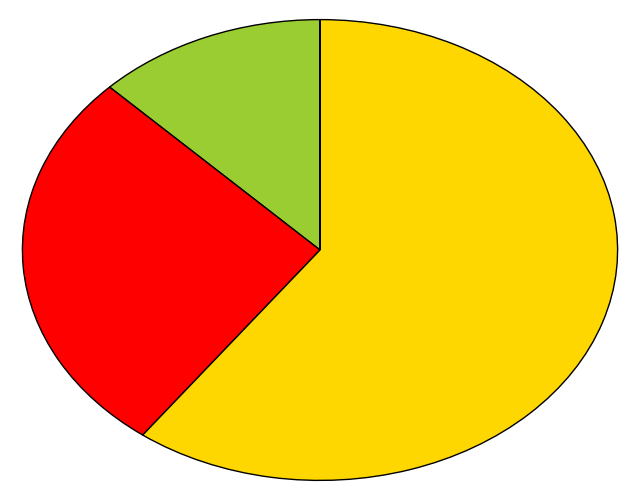
\includegraphics[width=\textwidth]{arousalEEGANOVA}
    \caption{ANOVA}
  \end{subfigure}
  \hfill
  \begin{subfigure}[b]{0.3\textwidth}
    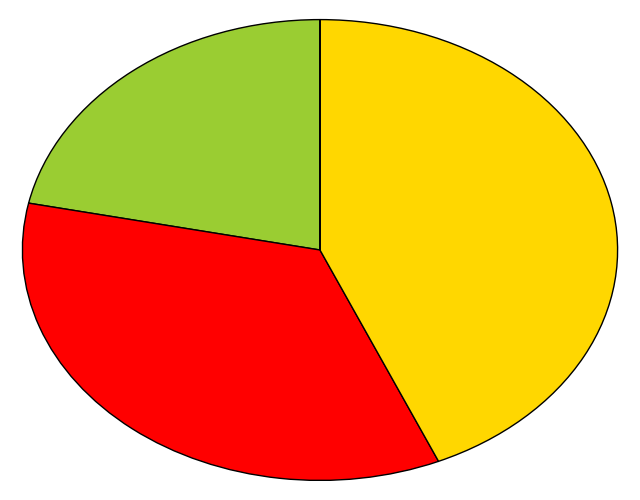
\includegraphics[width=\textwidth]{arousalEEGLR}
    \caption{Linear regression}
  \end{subfigure}
  \hfill
  \begin{subfigure}[b]{0.3\textwidth}
    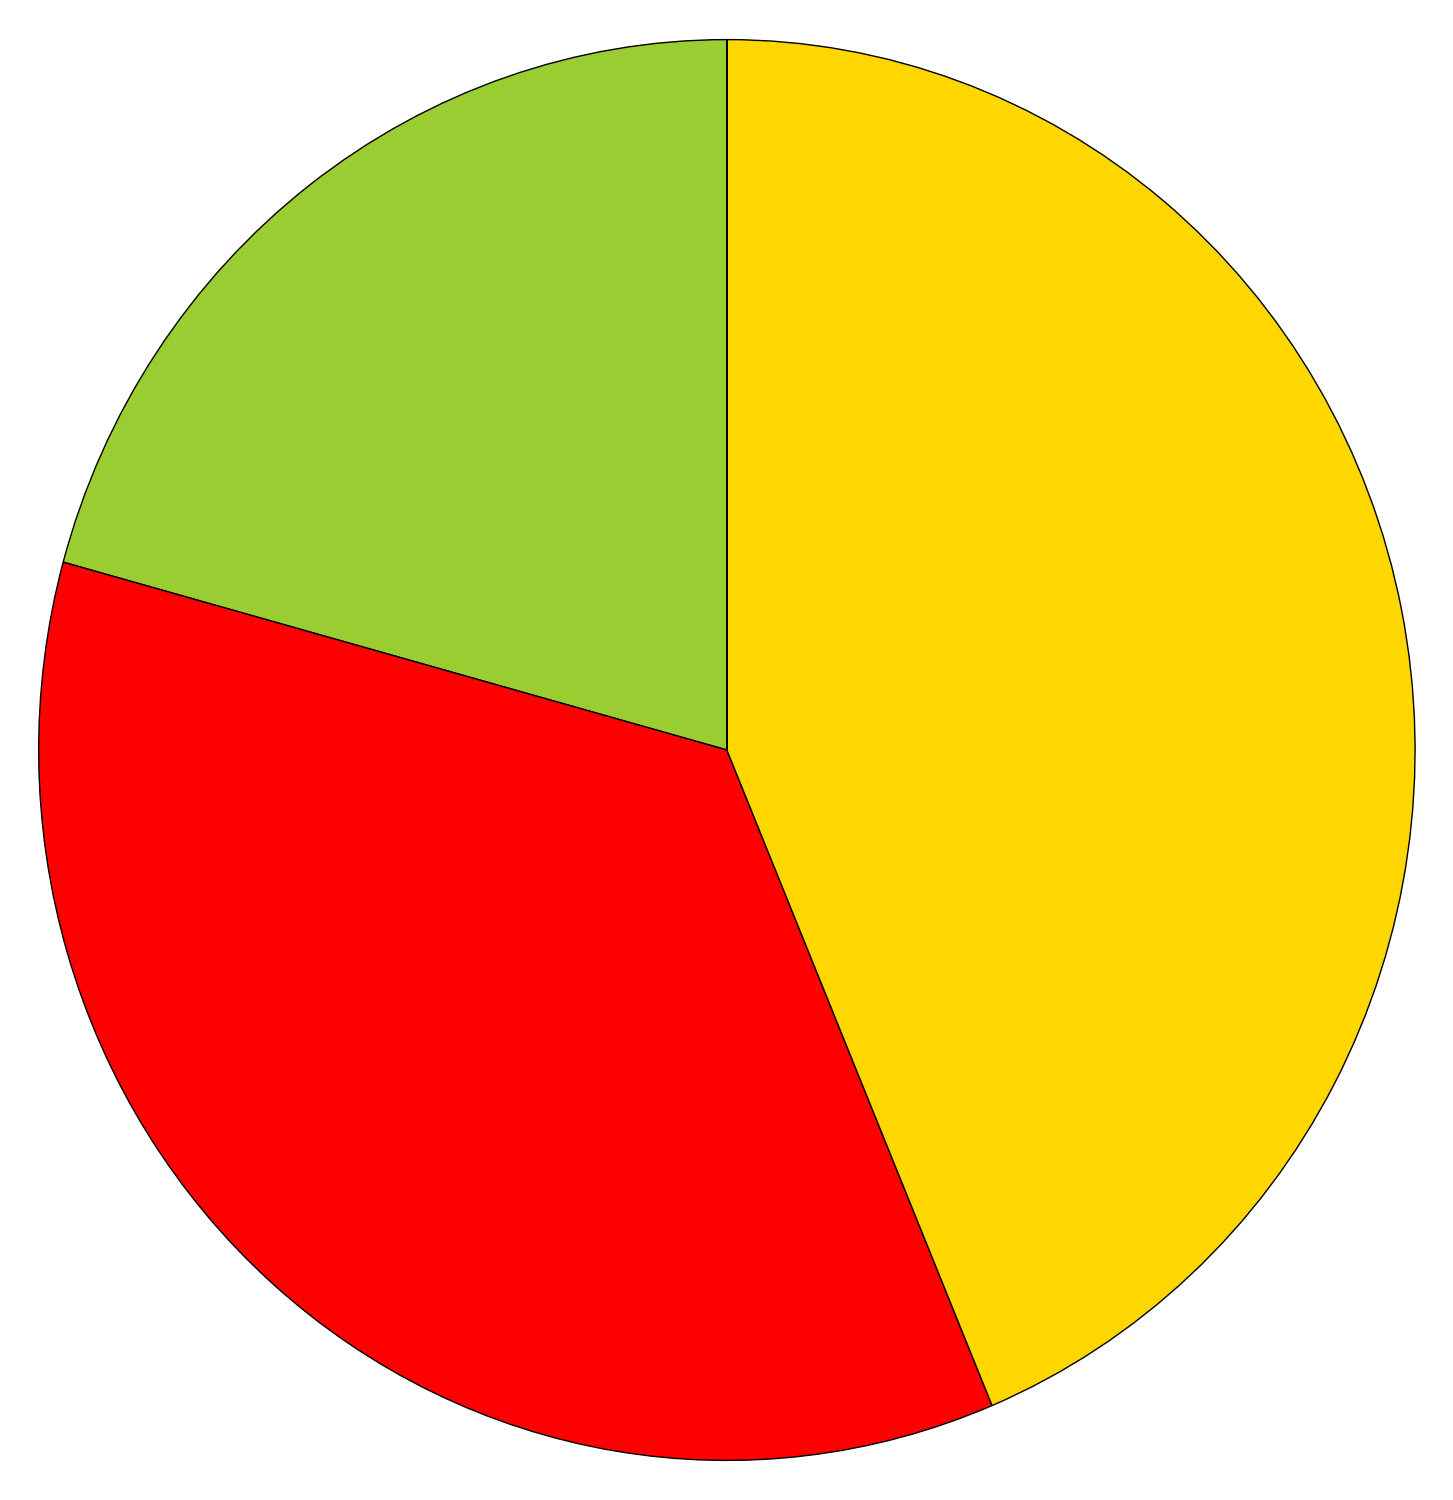
\includegraphics[width=\textwidth]{arousalEEGSVM}
    \caption{SVM}
  \end{subfigure}
  
  \begin{subfigure}[b]{0.3\textwidth}
    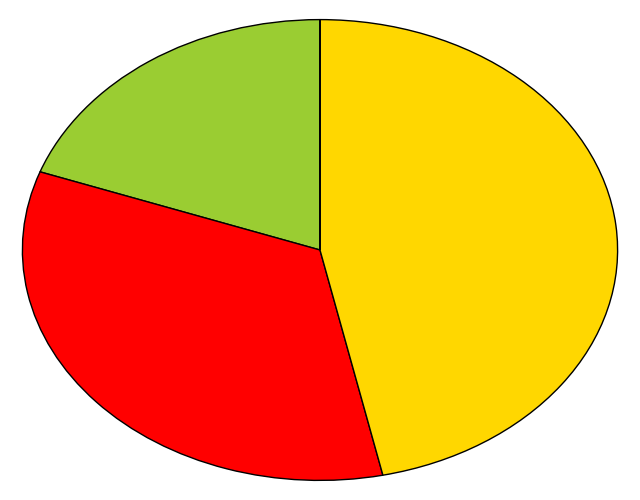
\includegraphics[width=\textwidth]{arousalEEGLDA}
    \caption{LDA}
  \end{subfigure}
  \hfill
  \begin{subfigure}[b]{0.3\textwidth}
    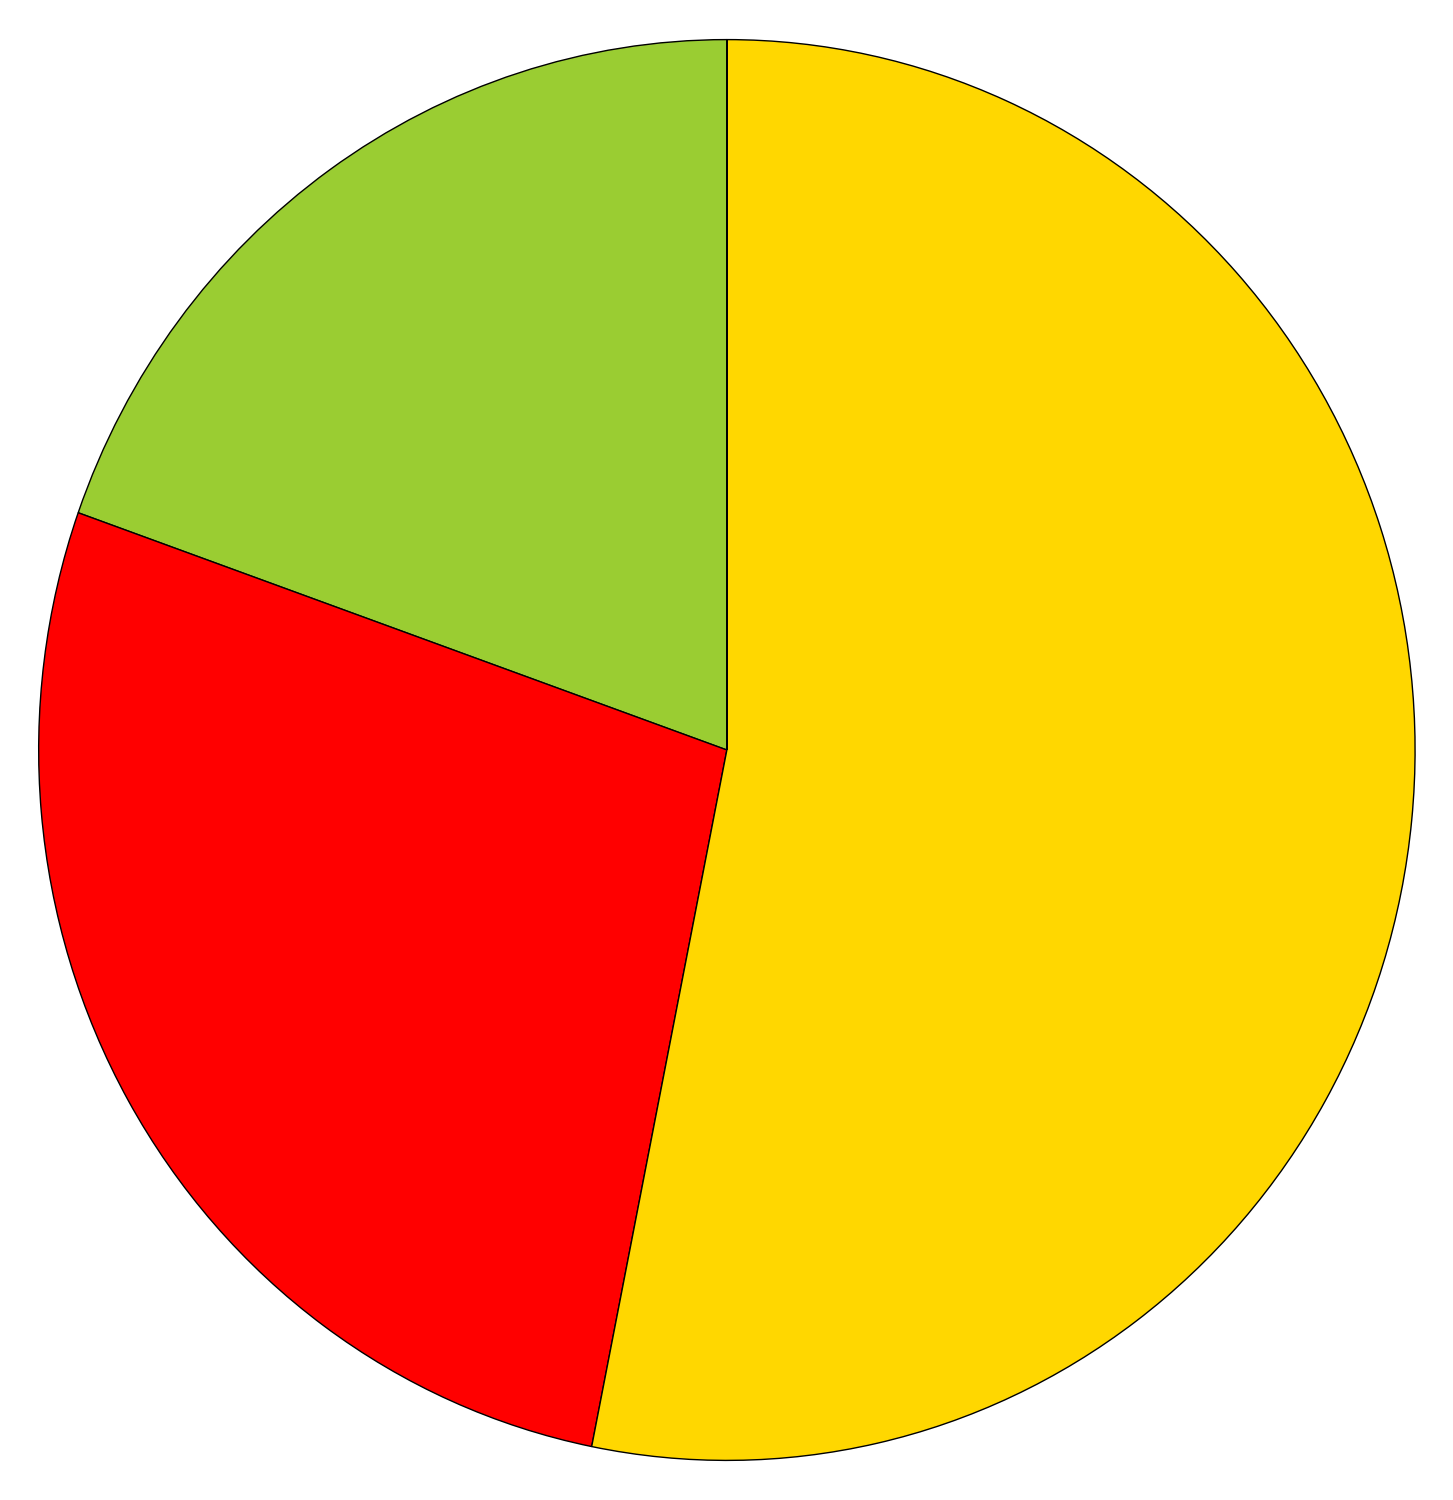
\includegraphics[width=\textwidth]{arousalEEGL1}
    \caption{Lasso regression}
  \end{subfigure}
  \hfill
  \begin{subfigure}[b]{0.3\textwidth}
    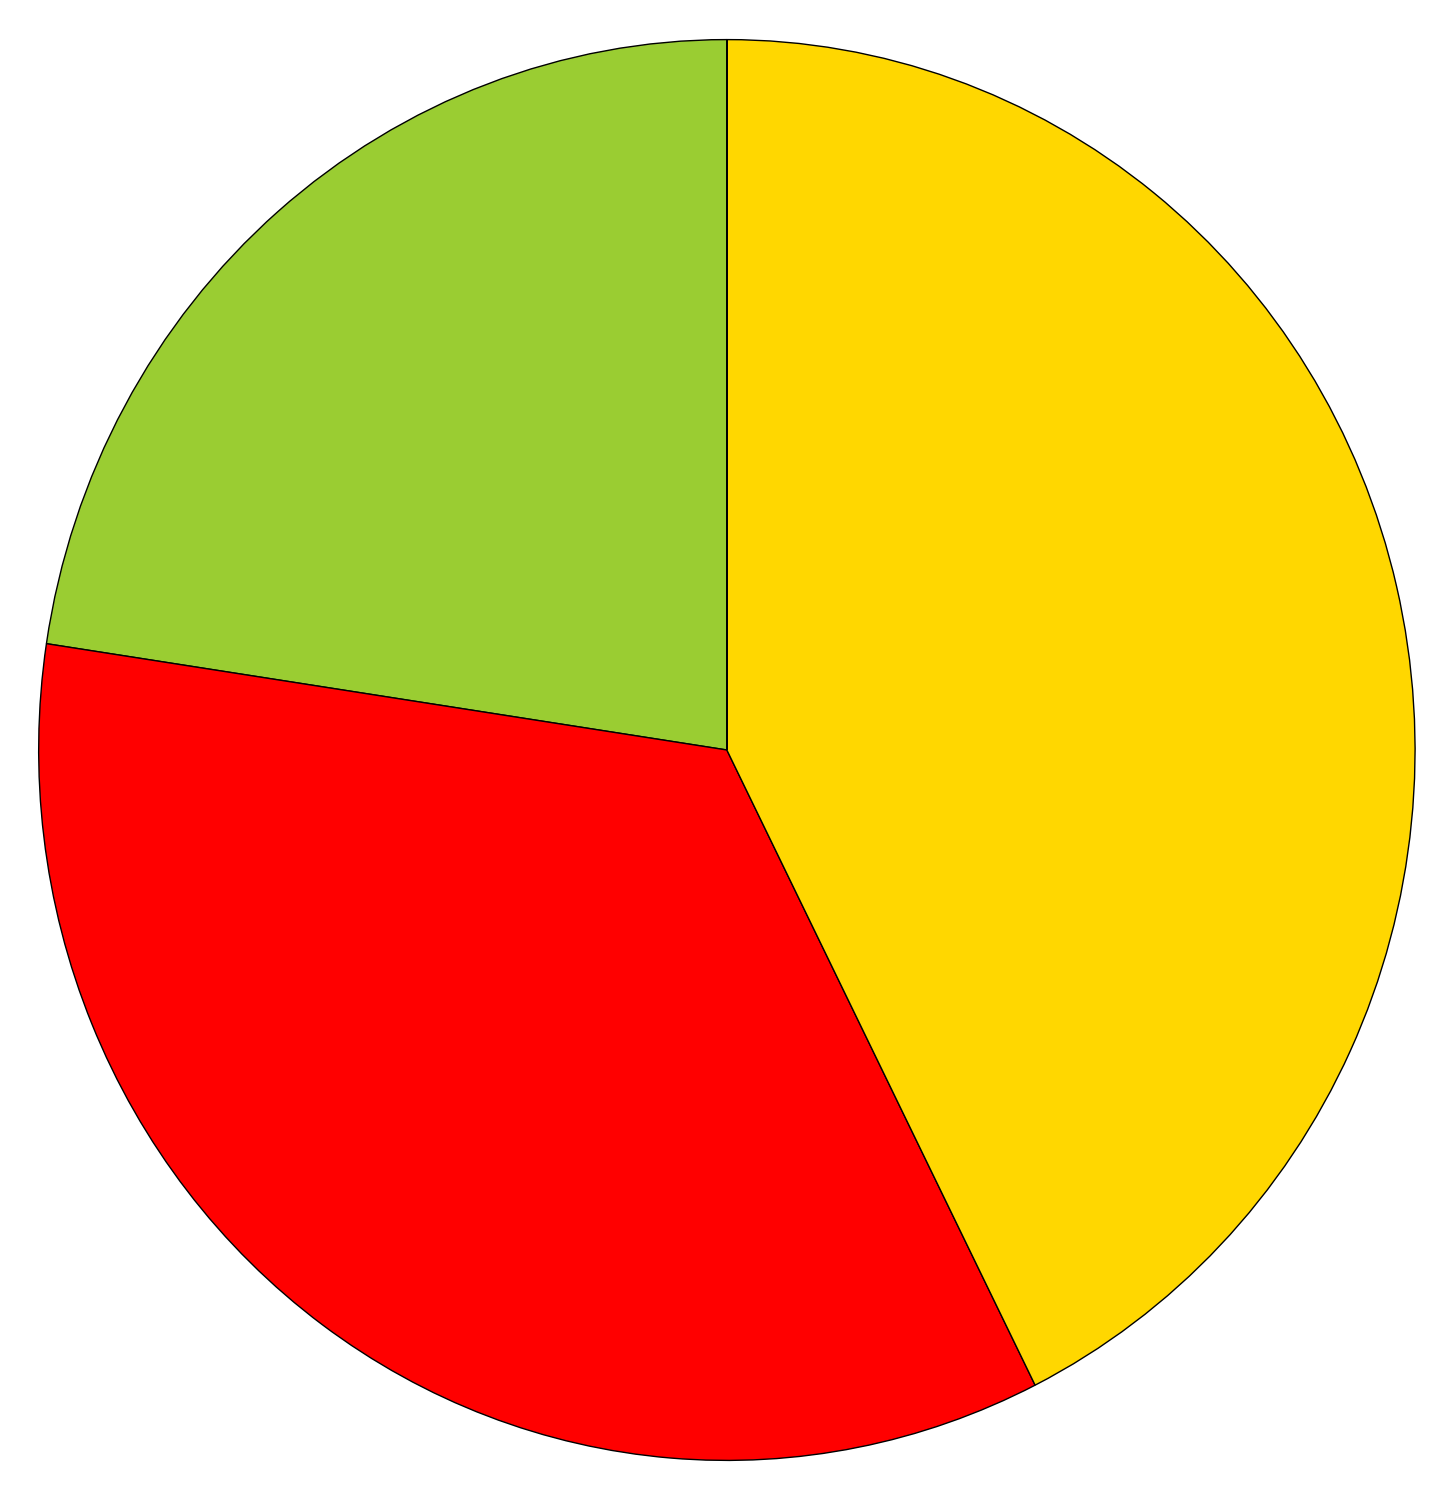
\includegraphics[width=\textwidth]{arousalEEGL2}
    \caption{Ridge regression}
  \end{subfigure}
  
  \begin{subfigure}[b]{0.3\textwidth}
    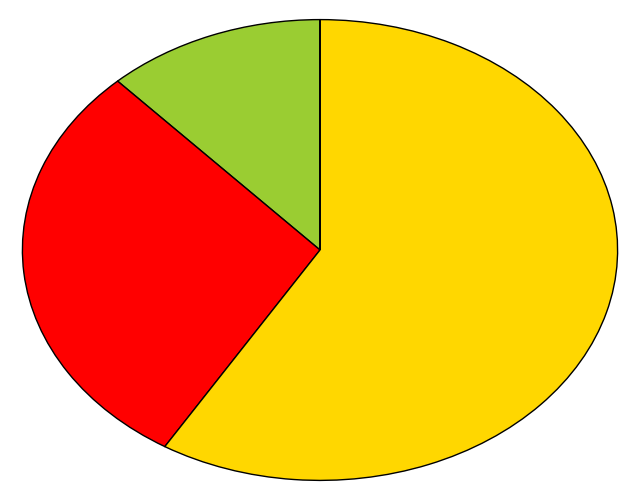
\includegraphics[width=\textwidth]{arousalEEGRF}
    \caption{Random forests}
  \end{subfigure}
  \hfill
  \begin{subfigure}[b]{0.3\textwidth}
    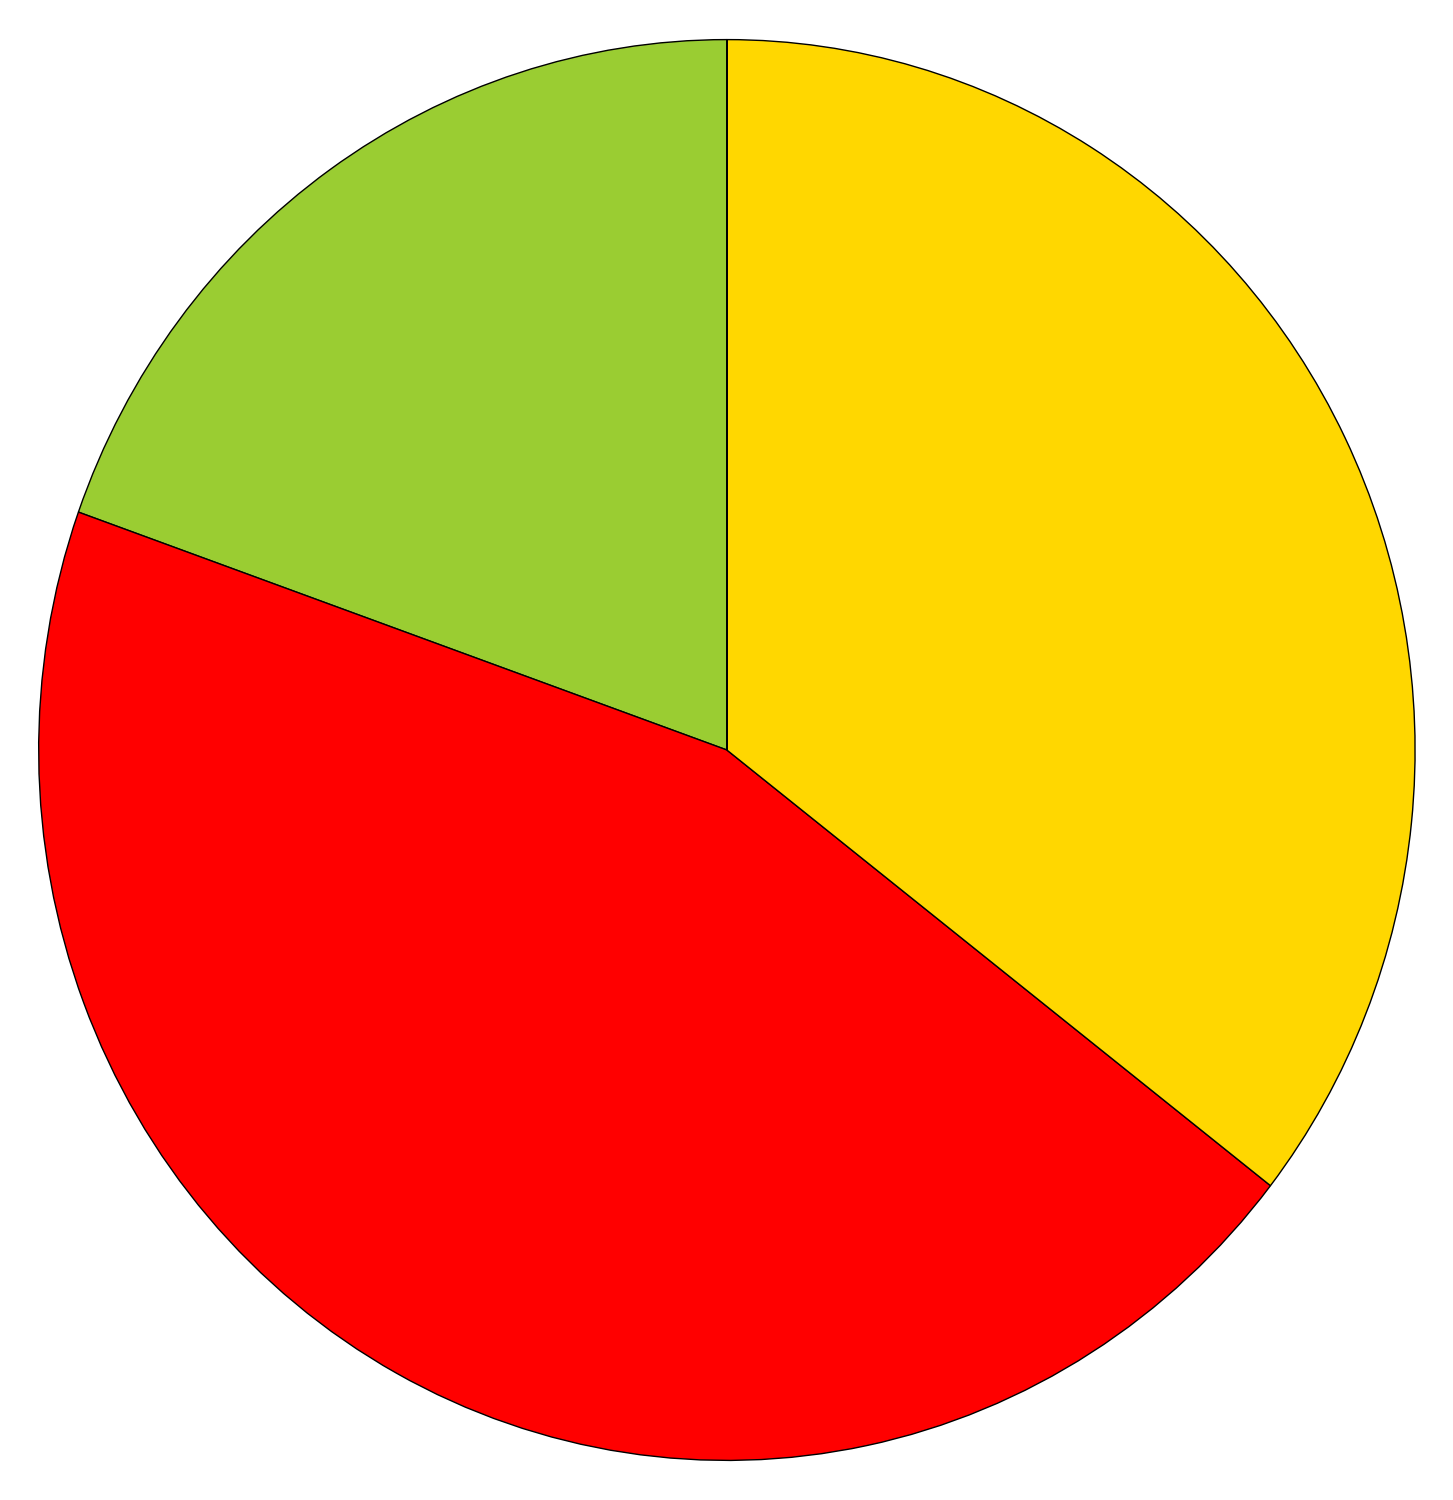
\includegraphics[width=\textwidth]{arousalEEGPCA}
    \caption{PCA}
  \end{subfigure}
  \hfill
  \begin{subfigure}[b]{0.3\textwidth}
    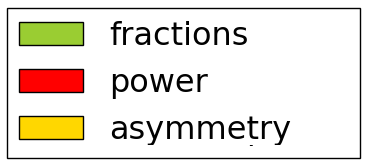
\includegraphics[width=\textwidth]{EEGlegend}
    \caption{Legend\label{arousalpiesEEGlegend}}
  \end{subfigure}
\end{figure}

\clearpage

\begin{figure}[!tbp]
  \centering
  \caption{Selection features for valence classification, using only EEG features.\label{valenceEEGpies}}
  \begin{subfigure}[b]{0.3\textwidth}
    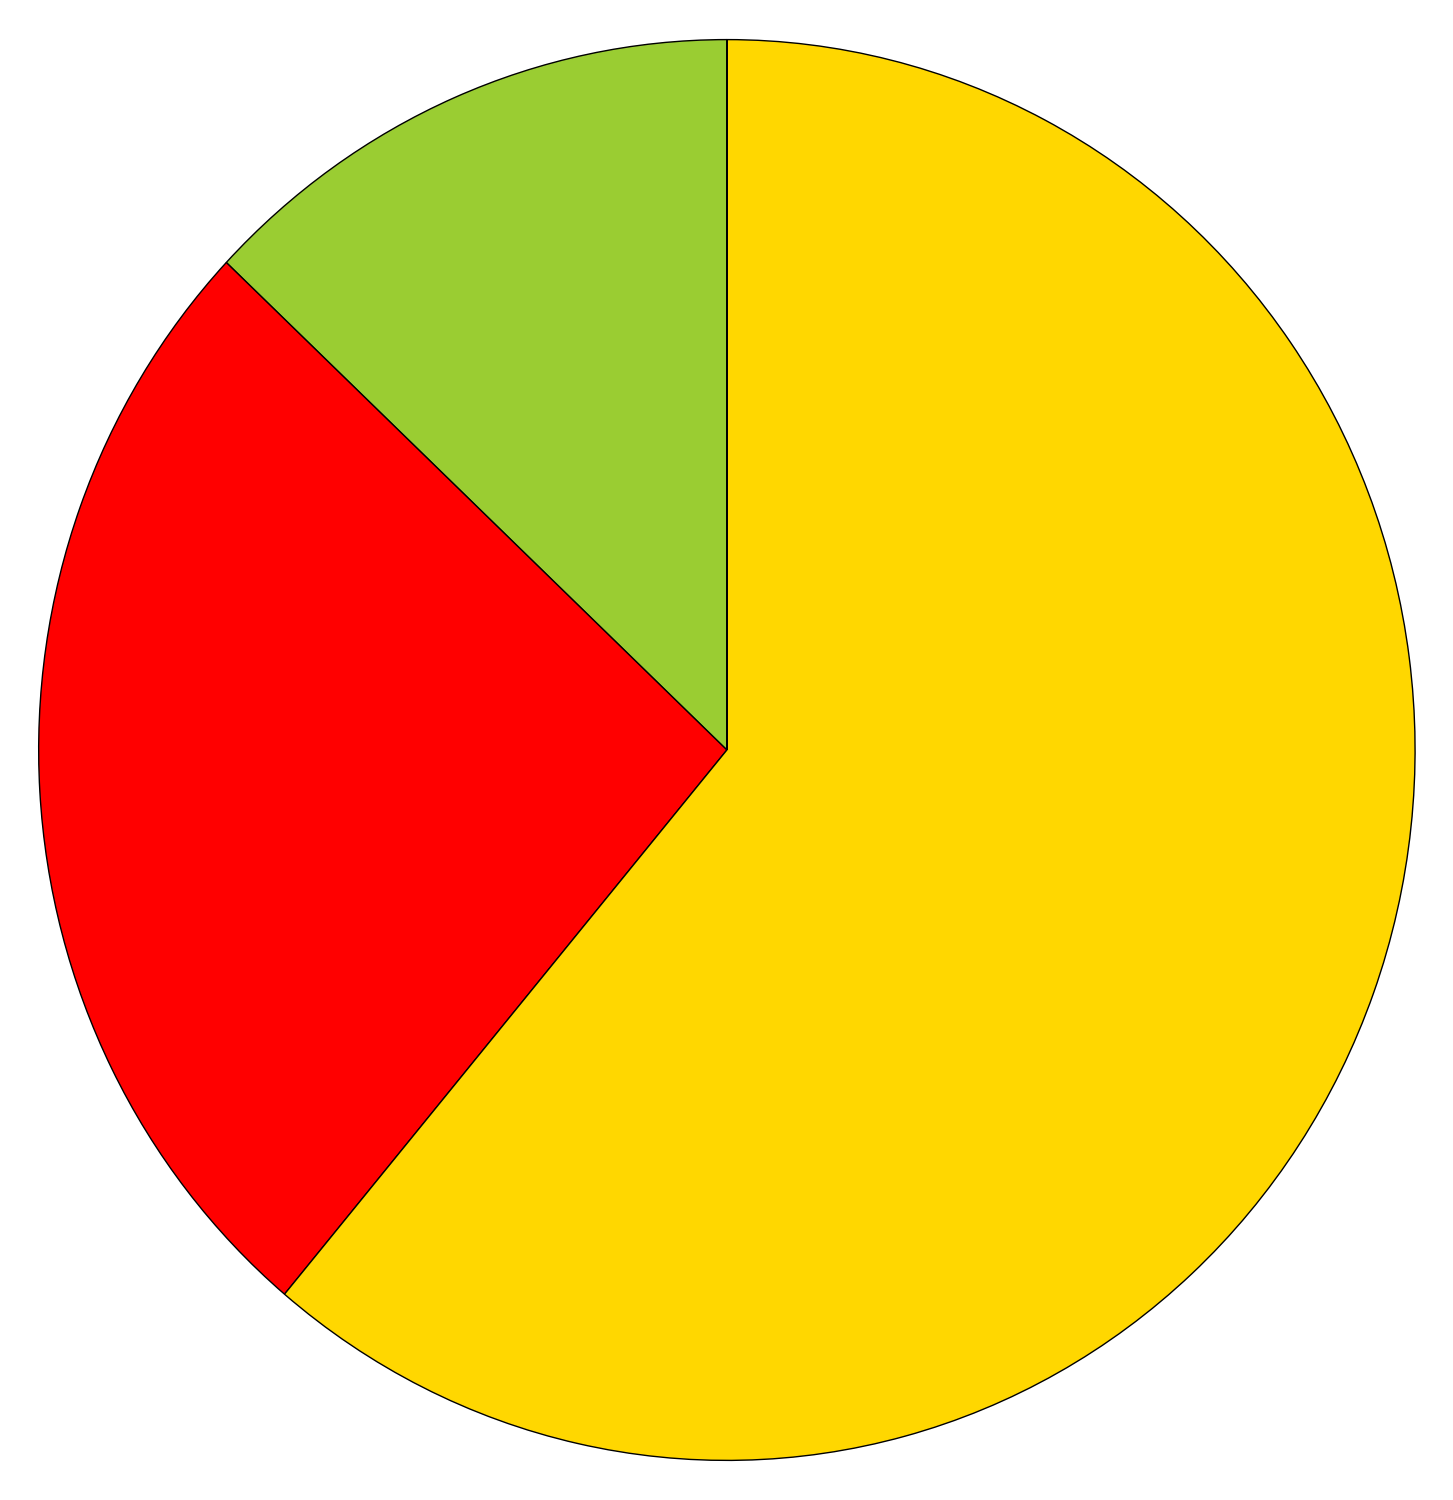
\includegraphics[width=\textwidth]{valenceEEGpearsonR}
    \caption{Pearson correlation}
  \end{subfigure}
  \hfill
  \begin{subfigure}[b]{0.3\textwidth}
    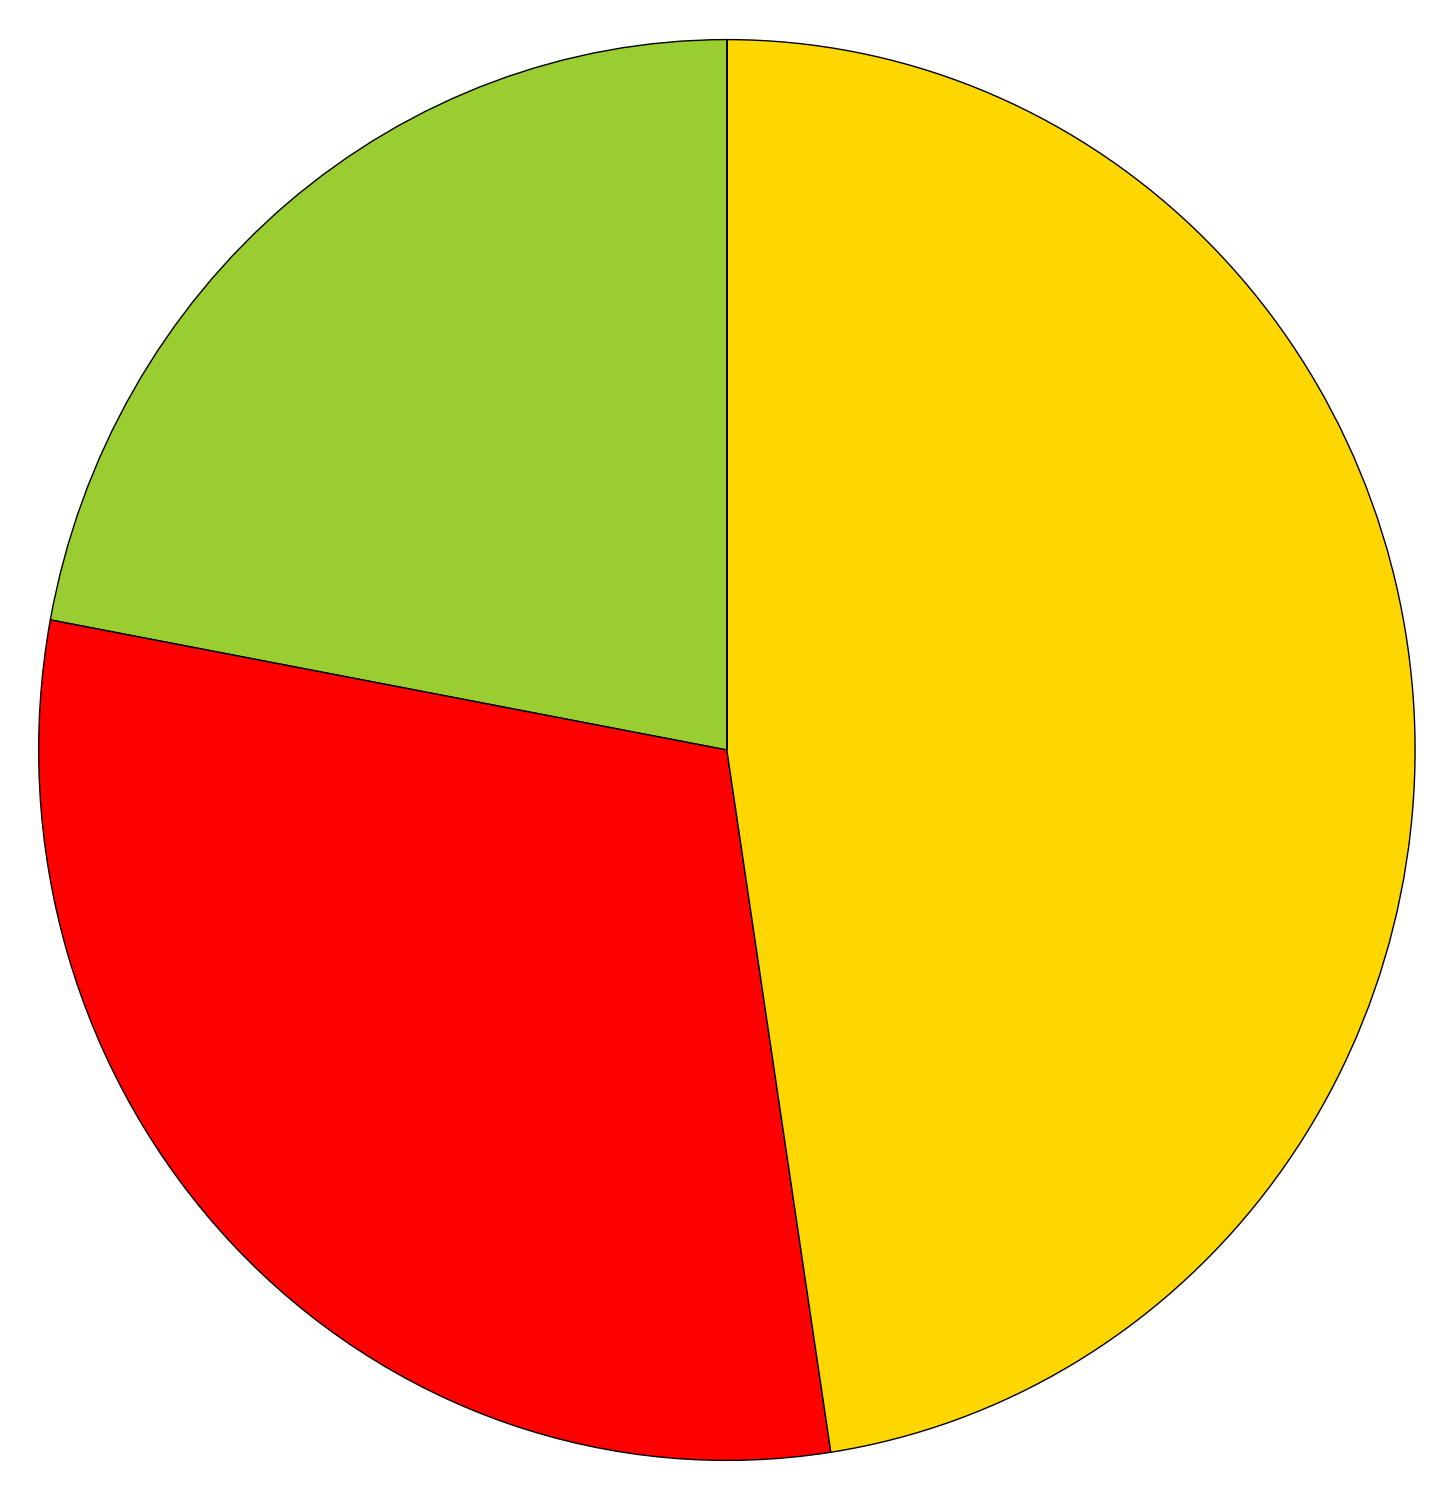
\includegraphics[width=\textwidth]{valenceEEGMutInf}
    \caption{Mutual information}
  \end{subfigure}
  \hfill
  \begin{subfigure}[b]{0.3\textwidth}
    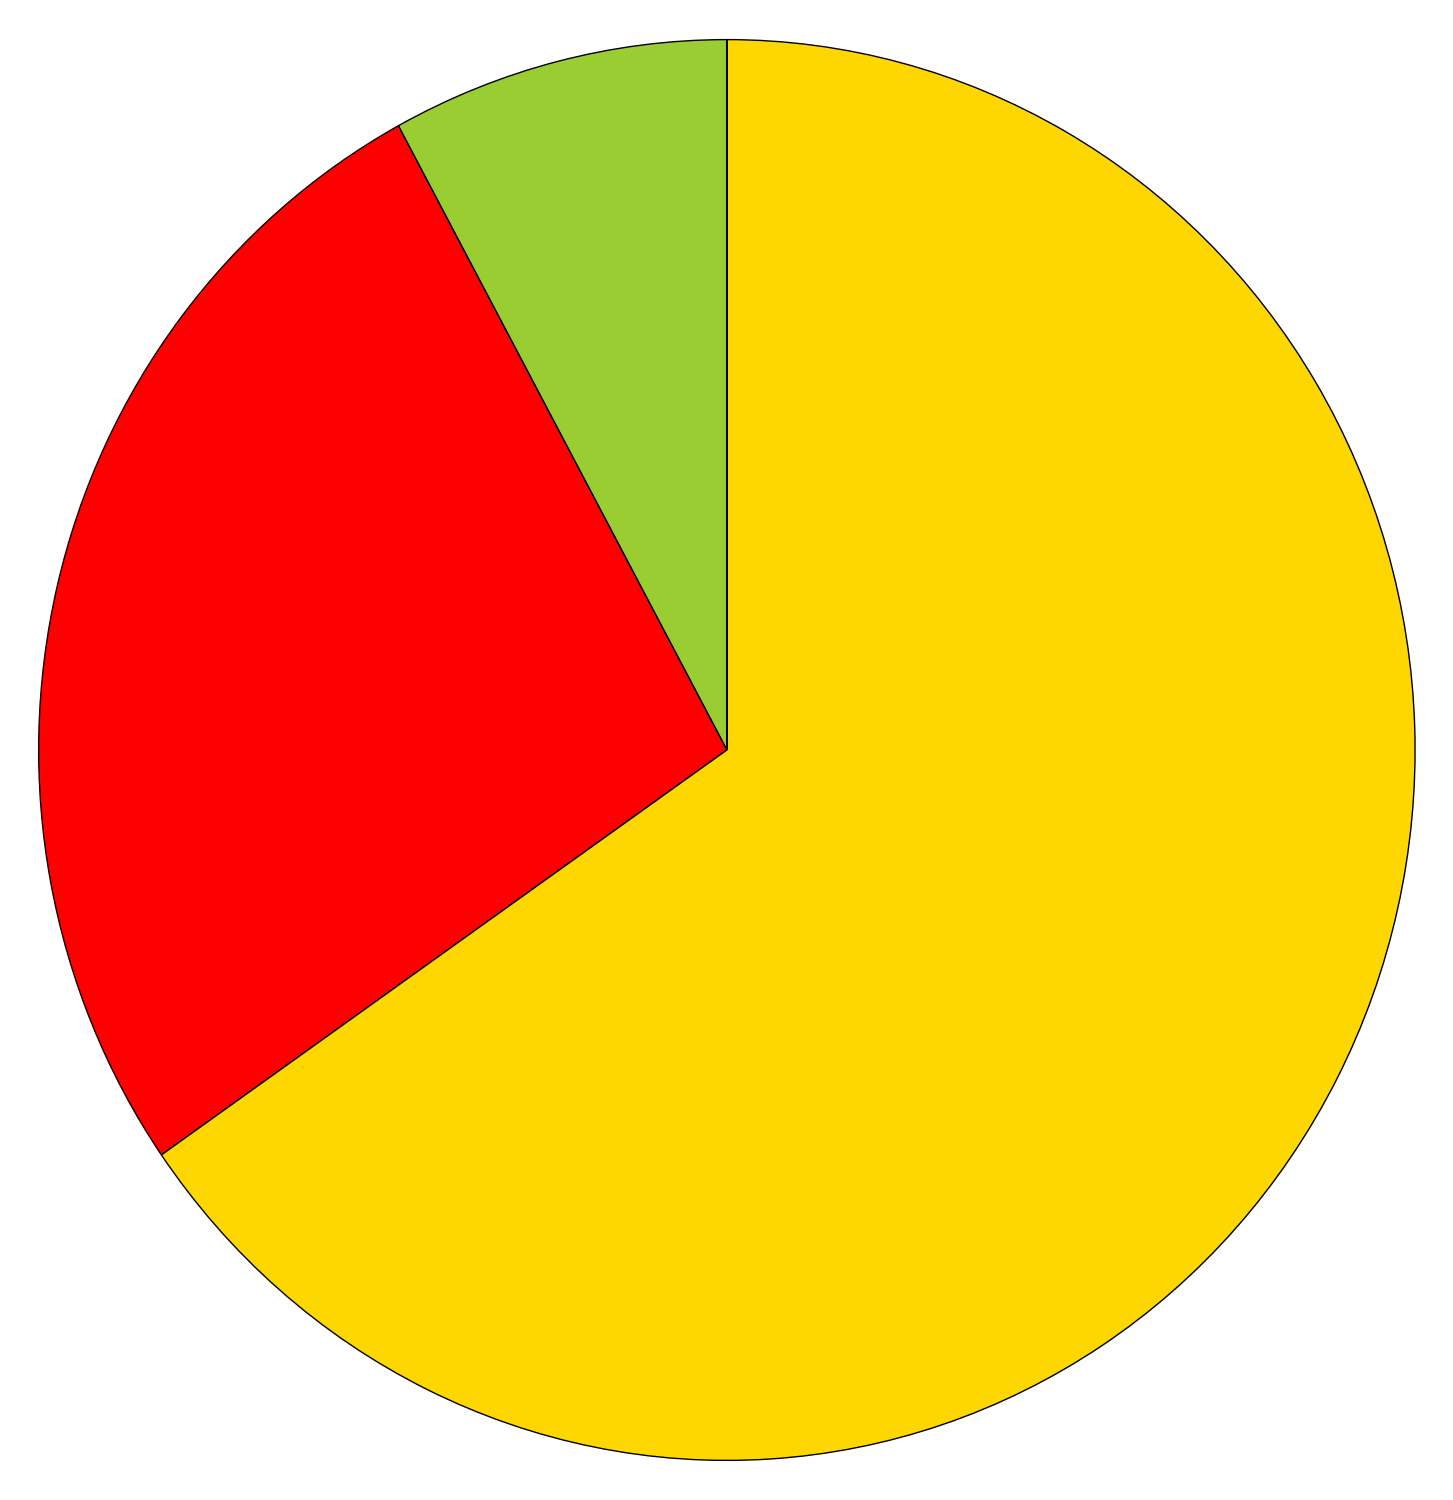
\includegraphics[width=\textwidth]{valenceEEGdCorr}
    \caption{Distance Correlation}
  \end{subfigure}
  
  \begin{subfigure}[b]{0.3\textwidth}
    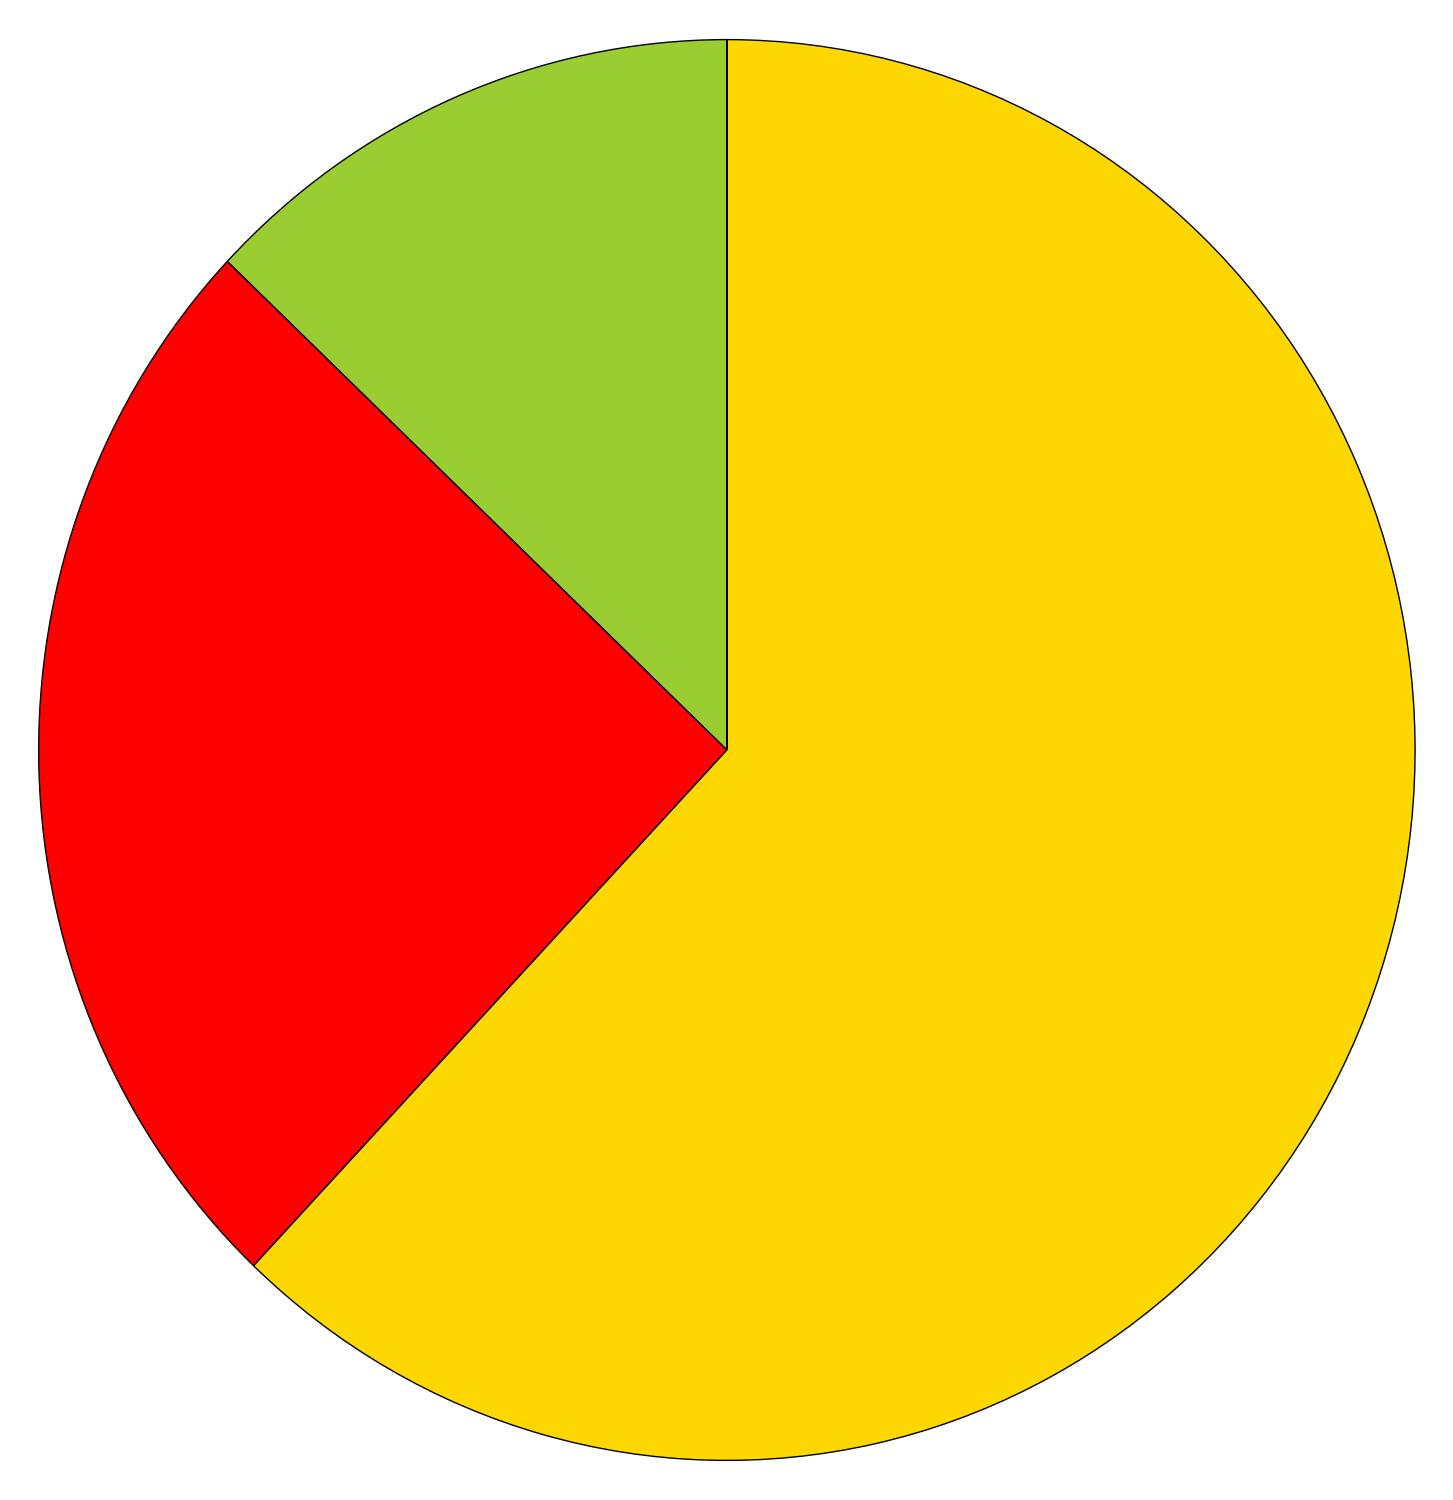
\includegraphics[width=\textwidth]{valenceEEGANOVA}
    \caption{ANOVA}
  \end{subfigure}
  \hfill
  \begin{subfigure}[b]{0.3\textwidth}
    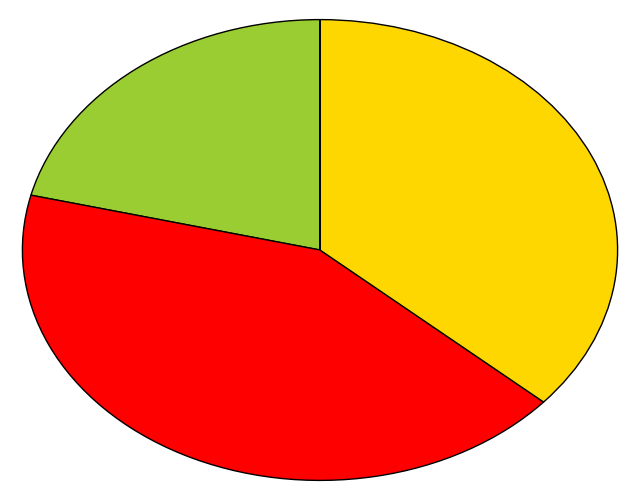
\includegraphics[width=\textwidth]{valenceEEGLR}
    \caption{Linear regression}
  \end{subfigure}
  \hfill
  \begin{subfigure}[b]{0.3\textwidth}
    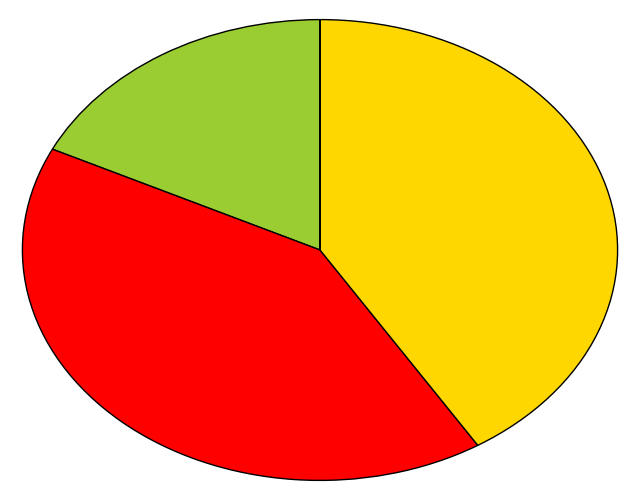
\includegraphics[width=\textwidth]{valenceEEGSVM}
    \caption{SVM}
  \end{subfigure}
  
  \begin{subfigure}[b]{0.3\textwidth}
    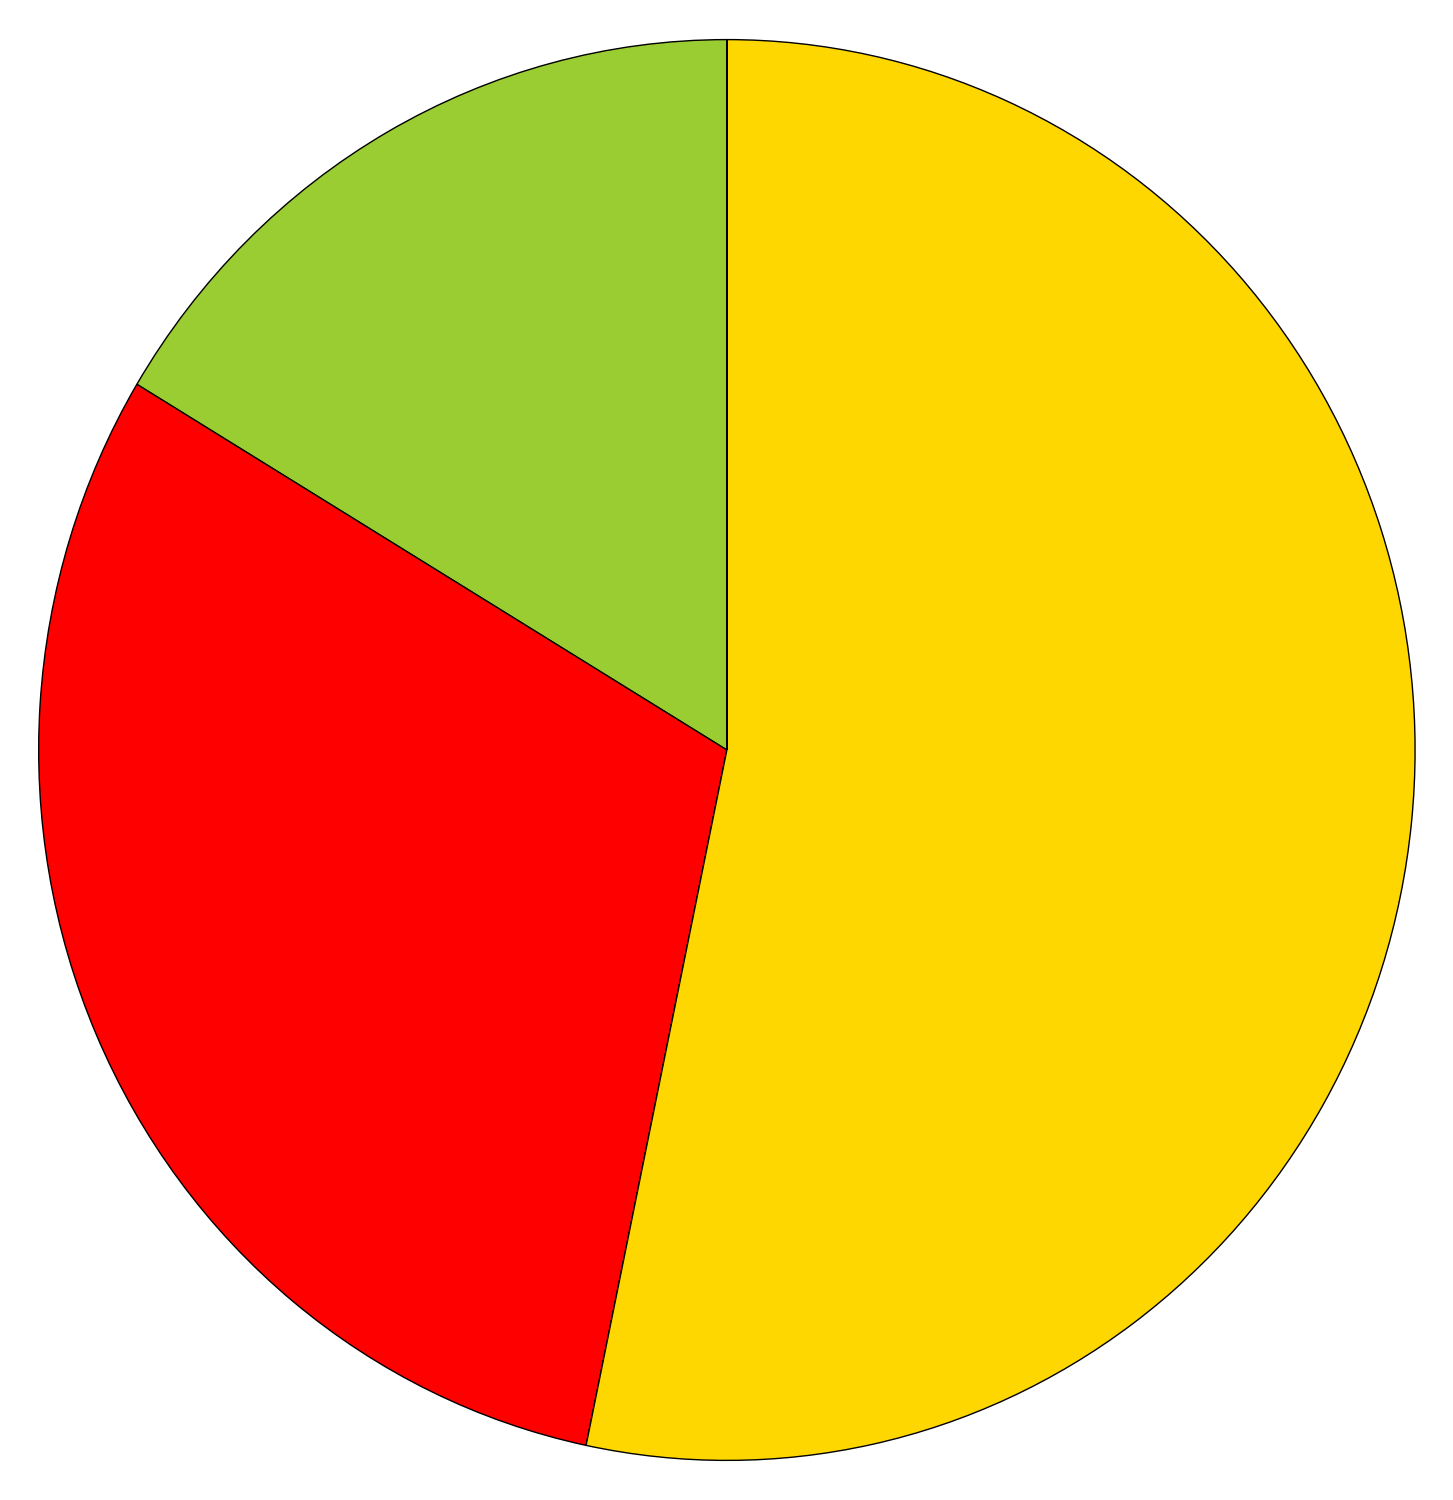
\includegraphics[width=\textwidth]{valenceEEGLDA}
    \caption{LDA}
  \end{subfigure}
  \hfill
  \begin{subfigure}[b]{0.3\textwidth}
    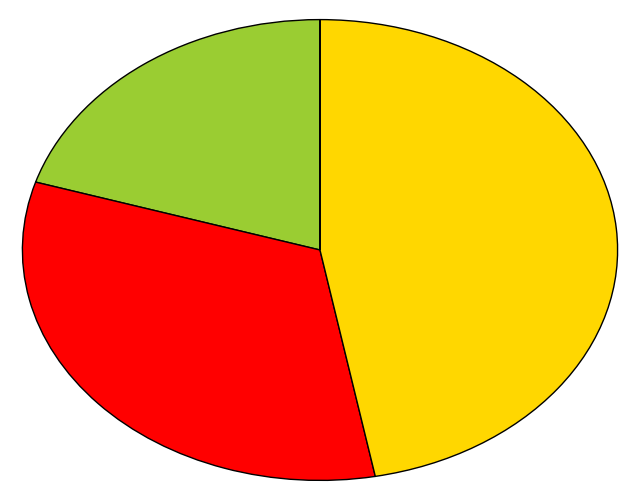
\includegraphics[width=\textwidth]{valenceEEGL1}
    \caption{Lasso regression}
  \end{subfigure}
  \hfill
  \begin{subfigure}[b]{0.3\textwidth}
    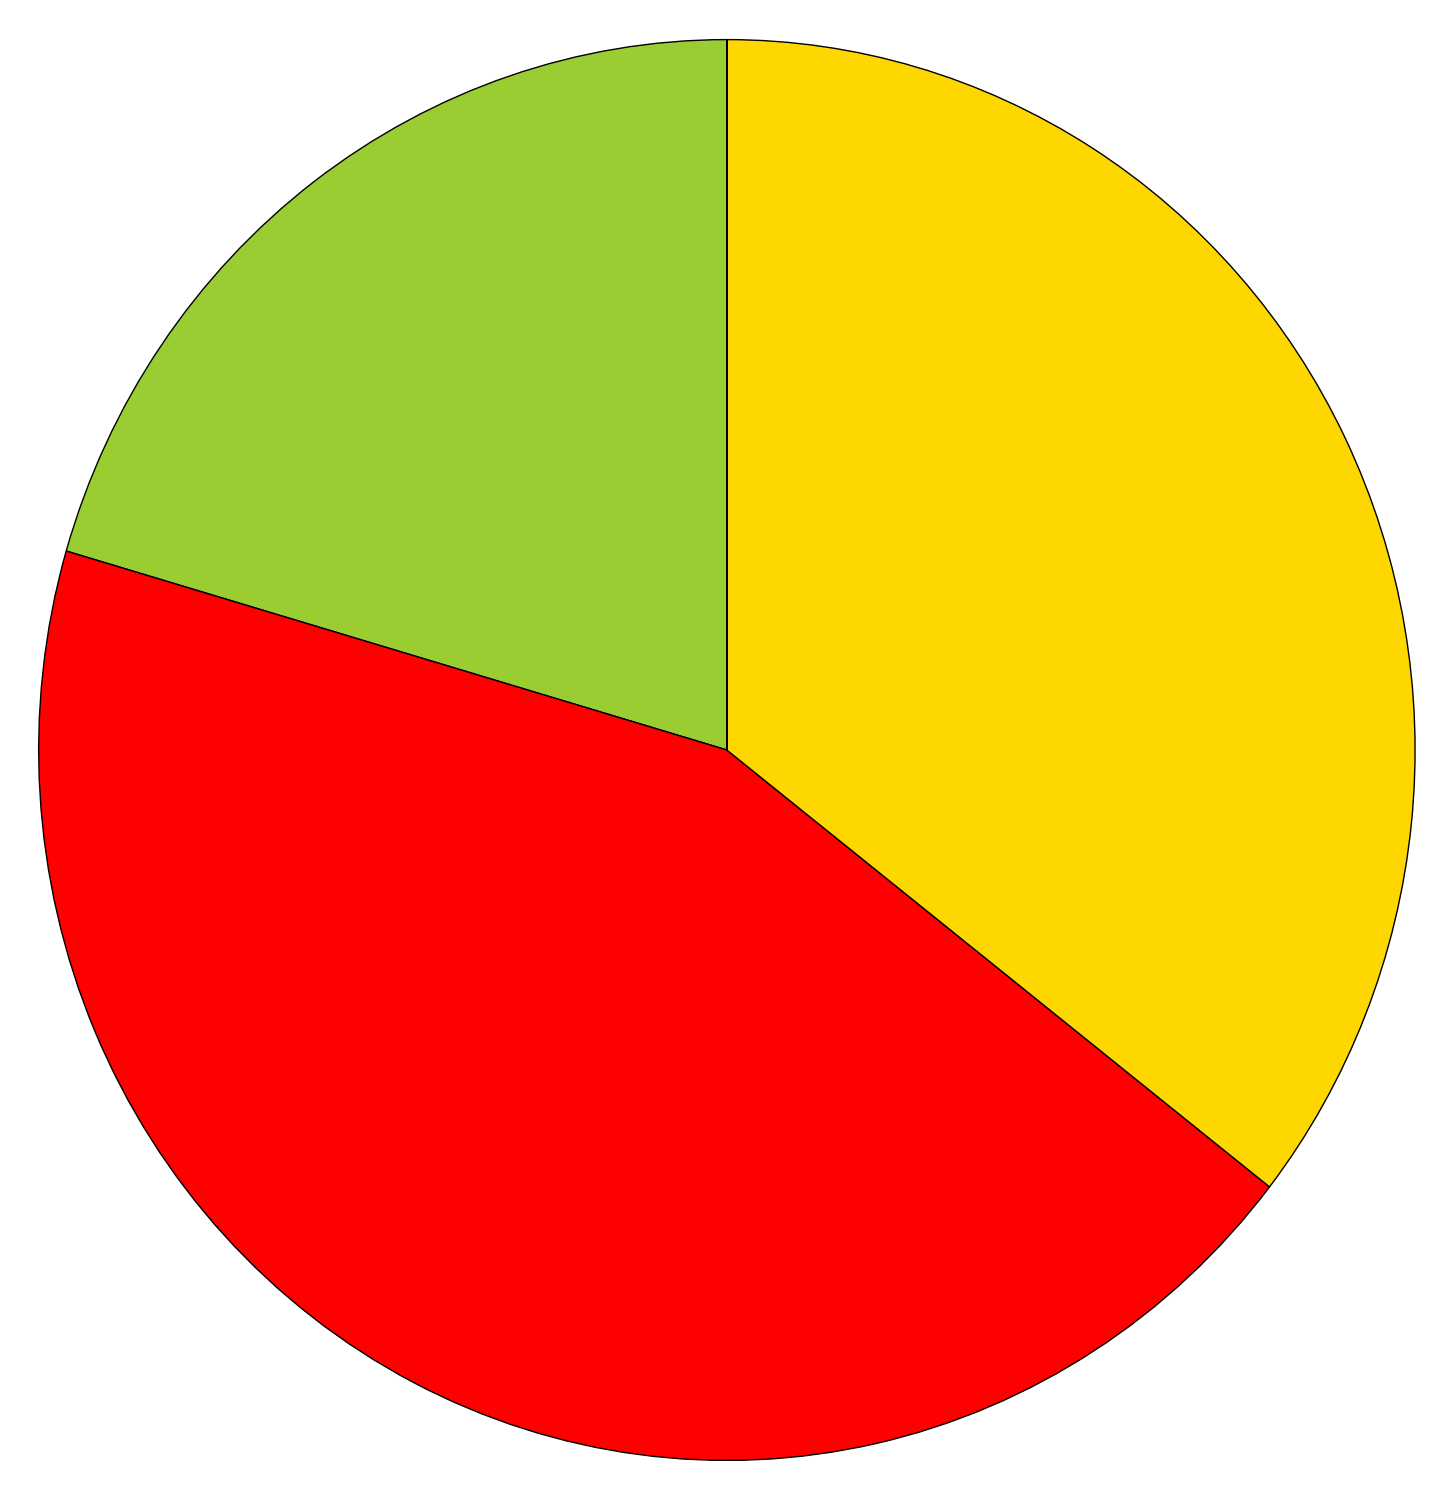
\includegraphics[width=\textwidth]{valenceEEGL2}
    \caption{Ridge regression}
  \end{subfigure}
  
  \begin{subfigure}[b]{0.3\textwidth}
    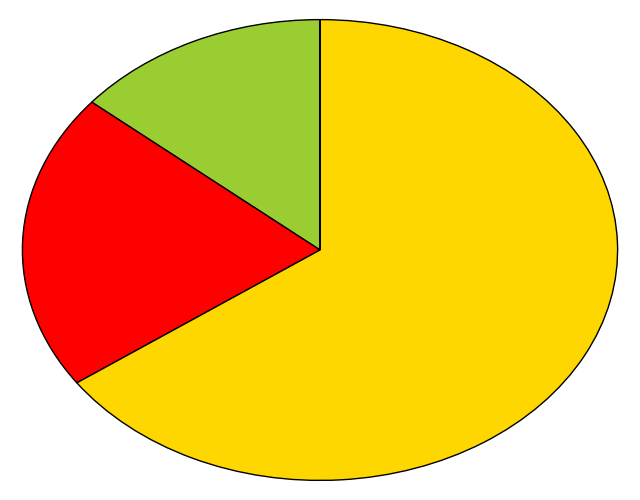
\includegraphics[width=\textwidth]{valenceEEGRF}
    \caption{Random forests}
  \end{subfigure}
  \hfill
  \begin{subfigure}[b]{0.3\textwidth}
    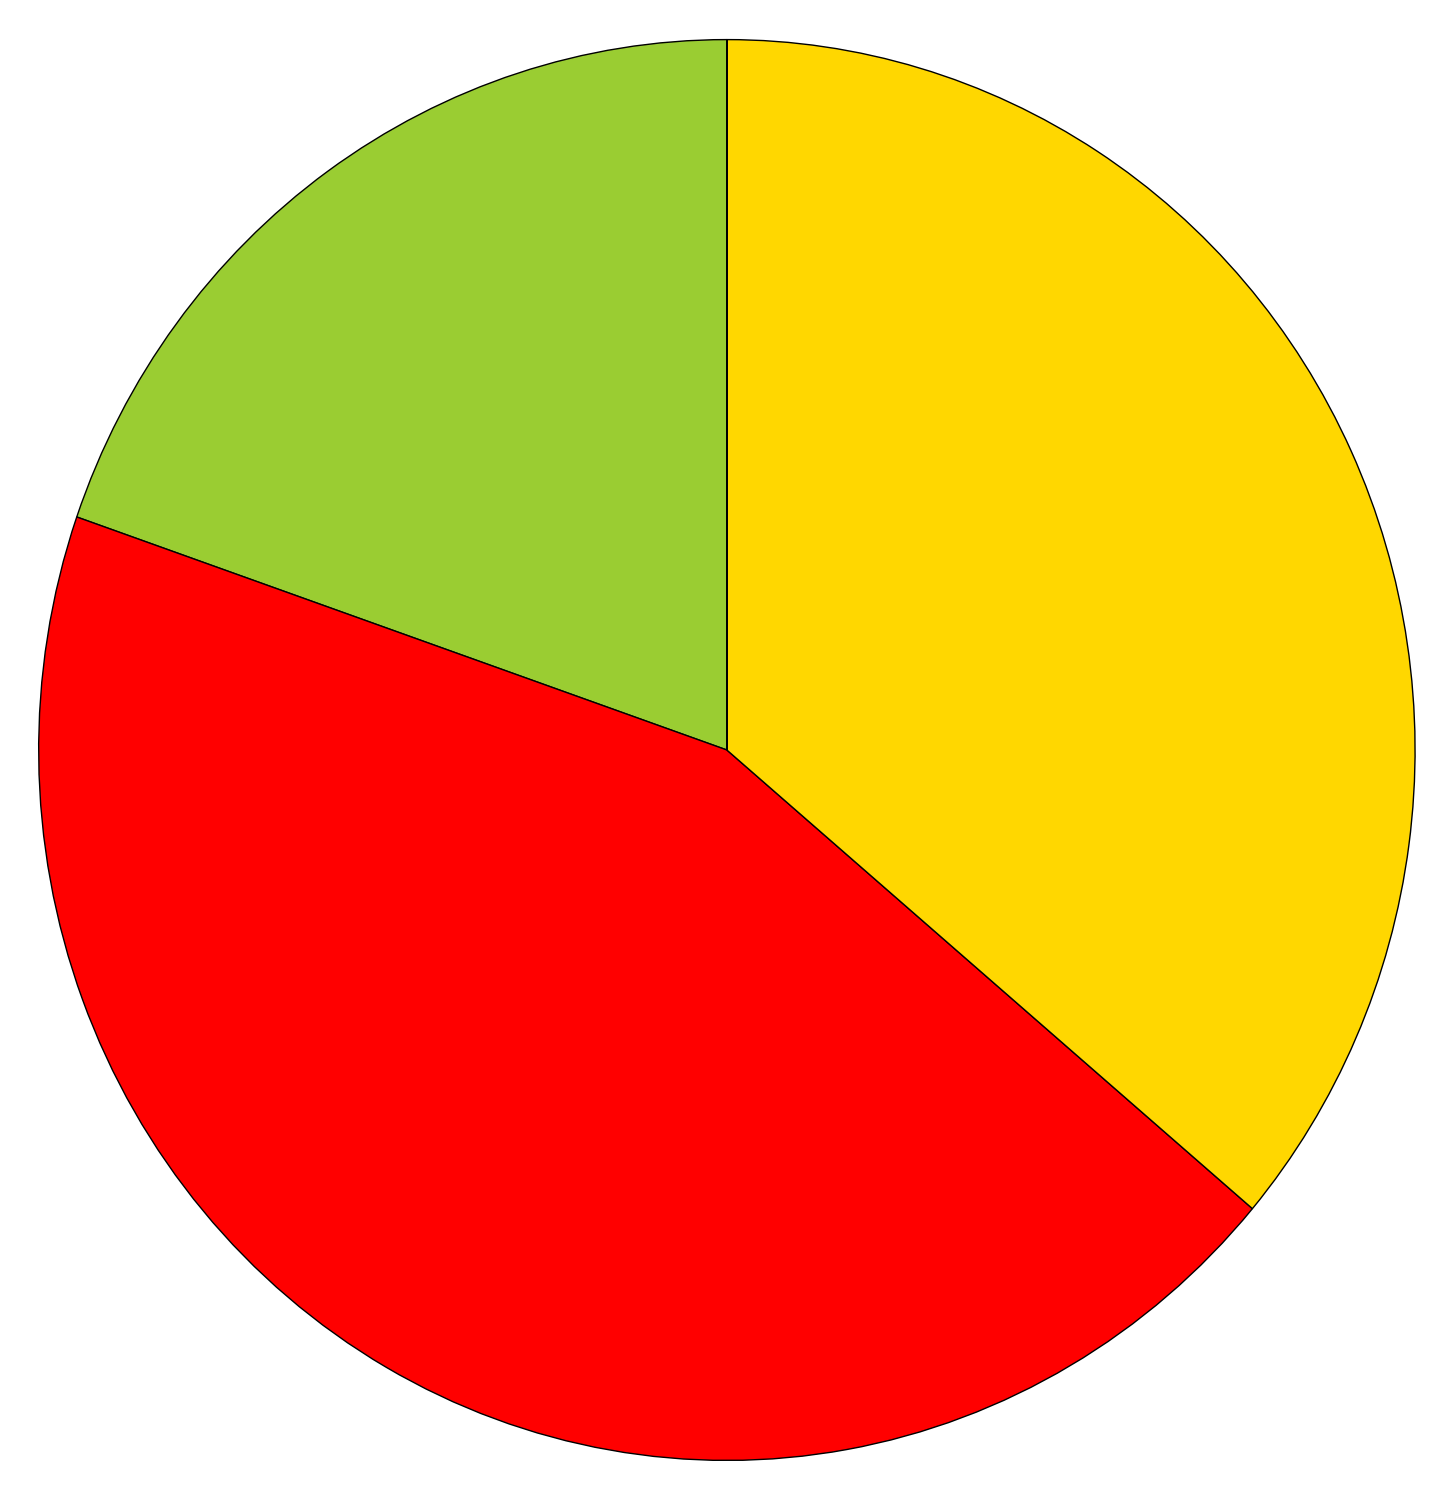
\includegraphics[width=\textwidth]{valenceEEGPCA}
    \caption{PCA}
  \end{subfigure}
  \hfill
  \begin{subfigure}[b]{0.3\textwidth}
    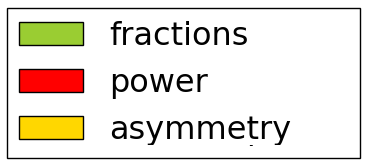
\includegraphics[width=\textwidth]{EEGlegend}
    \caption{Legend\label{valencepiesEEGlegend}}
  \end{subfigure}
\end{figure}
\clearpage

\begin{figure}[!tbp]
  \centering
  \caption{Selection features for arousal classification, using only non-EEG features.\label{arousalnon-EEGpies}}
  \begin{subfigure}[b]{0.3\textwidth}
    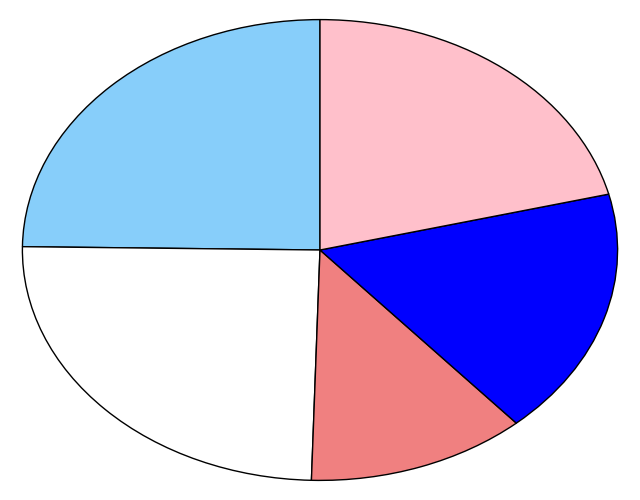
\includegraphics[width=\textwidth]{arousalnon-EEGpearsonR}
    \caption{Pearson correlation}
  \end{subfigure}
  \hfill
  \begin{subfigure}[b]{0.3\textwidth}
    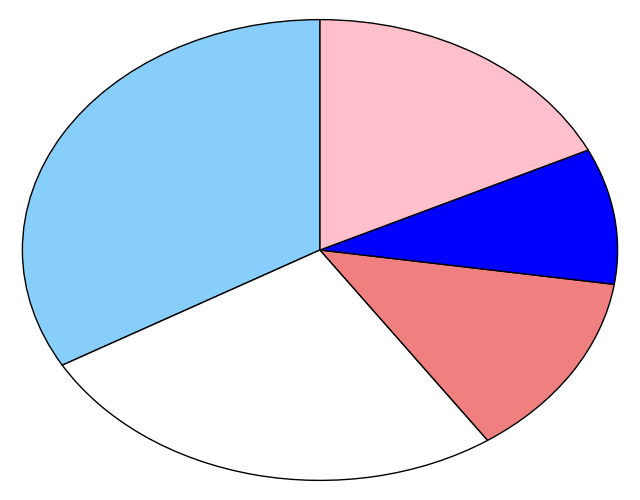
\includegraphics[width=\textwidth]{arousalnon-EEGMutInf}
    \caption{Mutual information}
  \end{subfigure}
  \hfill
  \begin{subfigure}[b]{0.3\textwidth}
    \includegraphics[width=\textwidth]{arousalnon-EEGdCorr}
    \caption{Distance Correlation}
  \end{subfigure}
  
  \begin{subfigure}[b]{0.3\textwidth}
    \includegraphics[width=\textwidth]{arousalnon-EEGANOVA}
    \caption{ANOVA}
  \end{subfigure}
  \hfill
  \begin{subfigure}[b]{0.3\textwidth}
    \includegraphics[width=\textwidth]{arousalnon-EEGLR}
    \caption{Linear regression}
  \end{subfigure}
  \hfill
  \begin{subfigure}[b]{0.3\textwidth}
    \includegraphics[width=\textwidth]{arousalnon-EEGSVM}
    \caption{SVM}
  \end{subfigure}
  
  \begin{subfigure}[b]{0.3\textwidth}
    \includegraphics[width=\textwidth]{arousalnon-EEGLDA}
    \caption{LDA}
  \end{subfigure}
  \hfill
  \begin{subfigure}[b]{0.3\textwidth}
    \includegraphics[width=\textwidth]{arousalnon-EEGL1}
    \caption{Lasso regression}
  \end{subfigure}
  \hfill
  \begin{subfigure}[b]{0.3\textwidth}
    \includegraphics[width=\textwidth]{arousalnon-EEGL2}
    \caption{Ridge regression}
  \end{subfigure}
  
  \begin{subfigure}[b]{0.3\textwidth}
    \includegraphics[width=\textwidth]{arousalnon-EEGRF}
    \caption{Random forests}
  \end{subfigure}
  \hfill
  \begin{subfigure}[b]{0.3\textwidth}
    \includegraphics[width=\textwidth]{arousalnon-EEGPCA}
    \caption{PCA}
  \end{subfigure}
  \hfill
  \begin{subfigure}[b]{0.3\textwidth}
    \includegraphics[width=\textwidth]{non-EEGlegend}
    \caption{Legend\label{arousalpiesnon-EEGlegend}}
  \end{subfigure}
\end{figure}

\clearpage

\begin{figure}[!tbp]
  \centering
  \caption{Selection features for valence classification, using only non-EEG features.\label{valencenon-EEGpies}}
  \begin{subfigure}[b]{0.3\textwidth}
    \includegraphics[width=\textwidth]{valencenon-EEGpearsonR}
    \caption{Pearson correlation}
  \end{subfigure}
  \hfill
  \begin{subfigure}[b]{0.3\textwidth}
    \includegraphics[width=\textwidth]{valencenon-EEGMutInf}
    \caption{Mutual information}
  \end{subfigure}
  \hfill
  \begin{subfigure}[b]{0.3\textwidth}
    \includegraphics[width=\textwidth]{valencenon-EEGdCorr}
    \caption{Distance Correlation}
  \end{subfigure}
  
  \begin{subfigure}[b]{0.3\textwidth}
    \includegraphics[width=\textwidth]{valencenon-EEGANOVA}
    \caption{ANOVA}
  \end{subfigure}
  \hfill
  \begin{subfigure}[b]{0.3\textwidth}
    \includegraphics[width=\textwidth]{valencenon-EEGLR}
    \caption{Linear regression}
  \end{subfigure}
  \hfill
  \begin{subfigure}[b]{0.3\textwidth}
    \includegraphics[width=\textwidth]{valencenon-EEGSVM}
    \caption{SVM}
  \end{subfigure}
  
  \begin{subfigure}[b]{0.3\textwidth}
    \includegraphics[width=\textwidth]{valencenon-EEGLDA}
    \caption{LDA}
  \end{subfigure}
  \hfill
  \begin{subfigure}[b]{0.3\textwidth}
    \includegraphics[width=\textwidth]{valencenon-EEGL1}
    \caption{Lasso regression}
  \end{subfigure}
  \hfill
  \begin{subfigure}[b]{0.3\textwidth}
    \includegraphics[width=\textwidth]{valencenon-EEGL2}
    \caption{Ridge regression}
  \end{subfigure}
  
  \begin{subfigure}[b]{0.3\textwidth}
    \includegraphics[width=\textwidth]{valencenon-EEGRF}
    \caption{Random forests}
  \end{subfigure}
  \hfill
  \begin{subfigure}[b]{0.3\textwidth}
    \includegraphics[width=\textwidth]{valencenon-EEGPCA}
    \caption{PCA}
  \end{subfigure}
  \hfill
  \begin{subfigure}[b]{0.3\textwidth}
    \includegraphics[width=\textwidth]{non-EEGlegend}
    \caption{Legend\label{valencepiesnon-EEGlegend}}
  \end{subfigure}
\end{figure}
\clearpage

\section{Important EEG channels}

Another component of this work is to dig into the EEG features and find out which channels are most important. This was done by taking the Random forest as a feature selection model and looking at the models that were build. By simply counting the occurrences of different EEG channels in these models, pie charts were constructed. This was done for both valence and arousal. The results are displayed in Figure\ref{arousalchannel} for arousal and Figure \ref{valencechannel} for valence.

\begin{figure}[H]
\centering

  \begin{subfigure}[b]{.5\textwidth}
    \includegraphics[width=\textwidth]{arousalchannel}
    \caption{The different selected channels for arousal.\label{arousalchannel}}
  \end{subfigure}
\hfill
  \begin{subfigure}[b]{.4\textwidth}
    \includegraphics[width=\textwidth]{channellegend}
    \caption{Each color and its corresponding EEG channel.}
  \end{subfigure}
\end{figure}

\begin{figure}[H]
\centering
  \begin{subfigure}[b]{.5\textwidth}
    \includegraphics[width=\textwidth]{valencechannel}
    \caption{The different selected channels for valence.\label{valencechannel}}
  \end{subfigure}
\hfill
  \begin{subfigure}[b]{.4\textwidth}
    \includegraphics[width=\textwidth]{channellegend}
    \caption{Each color and its corresponding EEG channel.}
  \end{subfigure}
\end{figure}

At first it seems that there is no agreement on the channels, one possible reason for this, might be that electrodes are not placed exactly. Even though the 10/20 system defines the different locations quite well, it is still possible that small variations in the locations exists. Grouping the channels might give a more clear view of the important regions of the brain. The channels were grouped as follows: 
\begin{table}[H]
\centering
\begin{tabular}{ll|ll|ll|ll}
\textbf{Channel} & \textbf{Region} & \textbf{Channel} & \textbf{Region} & \textbf{Channel} & \textbf{Region}      & \textbf{Channel} & \textbf{Region}     \\ \hline
\textbf{Fp1}     & front left      & \textbf{CP5}     & back left       & \textbf{Fp2}     & front right & \textbf{C4}      & back right \\
\textbf{AF3}     & front left      & \textbf{CP1}     & back left       & \textbf{AF4}     & front right & \textbf{T8}      & back right \\
\textbf{F3}      & front left      & \textbf{P3}      & back left       & \textbf{Fz}      & midline     & \textbf{CP6}     & back right \\
\textbf{F7}      & front left      & \textbf{P7}      & back left       & \textbf{F4}      & front right & \textbf{CP2}     & back right \\
\textbf{FC5}     & front left      & \textbf{PO3}     & back left       & \textbf{F8}      & front right & \textbf{P4}      & back right \\
\textbf{FC1}     & front left      & \textbf{O1}      & back left       & \textbf{FC6}     & front right & \textbf{P8}      & back right \\
\textbf{C3}      & back left       & \textbf{Oz}      & midline         & \textbf{FC2}     & front right & \textbf{PO4}     & back right \\
\textbf{T7}      & back left       & \textbf{Pz}      & midline         & \textbf{Cz}      & midline     & \textbf{O2}      & back right
\end{tabular}
\caption{The region for each EEG channel}
\end{table}

These Region are also depicted in Figure \ref{regions}.
\mijnfiguur{width=.8\textwidth}{regions}{All EEG channels were grouped in 4 regions: left-front (blue), right-front (red), left-back(black), right-back (purple) and midline (yellow).}

The resulting distributions are shown in Figure \ref{arousalzones} for arousal and in Figure \ref{valencezones}, the legend is shown in Figure \ref{zonelegend}.

\begin{figure}[H]
\centering
  \begin{subfigure}[b]{.4\textwidth}
    \includegraphics[width=\textwidth]{arousalzones}
    \caption{Origin of the power features for arousal classification.\label{arousalzones}}
  \end{subfigure}
\hfill
  \begin{subfigure}[b]{.4\textwidth}
    \includegraphics[width=\textwidth]{valencezones}
    \caption{Origin of the power features for valence classification.\label{valencezones}}
  \end{subfigure}
\\
  \begin{subfigure}[b]{.7\textwidth}
    \includegraphics[width=\textwidth]{zonelegend}
    \caption{The corresponding zone for each color.\label{zonelegend}}
  \end{subfigure}
\end{figure}

Looking at the pie plots, one can see that there is no clear region used. The back left and right regions appear most often, but the difference with the front left and right is little. It seems that for both valence and arousal, power values of all different regions might be of importance. The distributions for the regions are the same for both valence and arousal, but they differ in terms of channels.

\npar

The same principle can be done for the asymmetry features, here a distinction was made between DASM and RASM features on one hand and the DCAU and RCAU features on the other hand. The DASM and RASM features were divided in channel pairs located at the front and back of the brain. A specific list is given in Table \ref{ASMgroupTable} below.

%table
\begin{table}[H]
\centering
\begin{tabular}{ll|ll}
\textbf{Channel pair} & \textbf{Group} & \textbf{Channel pair} & \textbf{Group} \\ \hline
Fp1,Fp2               & front          & C3,C4                 & back           \\
AF3,AF4               & front          & T7,T8                 & back           \\
F3,F4                 & front          & CP5,CP6               & back           \\
F7,F8                 & front          & CP1,CP2               & back           \\
FC5,FC6               & front          & P3,P4                 & back           \\
FC1,FC2               & front          & P7,P8                 & back           \\
                      &                & PO3,PO4               & back          
\end{tabular}
\caption{the region for each DASM and RASM channel pair\label{ASMgroupTable}}
\end{table}

\begin{figure}[H]
\centering
  \begin{subfigure}[b]{.4\textwidth}
    \includegraphics[width=\textwidth]{arousalasymzonesASM}
    \caption{Origin of the asymmetry features for arousal classification.\label{arousalasymzonesASM}}
  \end{subfigure}
\hfill
  \begin{subfigure}[b]{.4\textwidth}
    \includegraphics[width=\textwidth]{valenceasymzonesASM}
    \caption{Origin of the asymmetry features for valence classification.\label{valenceasymzonesASM}}
  \end{subfigure}
\\
  \begin{subfigure}[b]{.4\textwidth}
    \includegraphics[width=\textwidth]{ASMlegend}
    \caption{The corresponding zone for each color.\label{ASMlegend}}
  \end{subfigure}
\end{figure}

For the DASM and RASM features, it is clear that the asymmetry should be measured at the front of the scalp for arousal. For valence however, features are selected from the front and the back of the scalp. This is in contradiction with the literature, most studies suggest that the frontal asymmetry of alpha power is most valuable.

\npar

The caudality features also measure asymmetry, but between a frontal and posterior channel. Here, the channel pairs were grouped in three groups: left, right and Fz/PZ, since the Fz/Pz channel pair lies on the central line. The specific grouping is shown in Table \ref{CAUgroupTable} below.

%table
\begin{table}[H]
\centering
\begin{tabular}{ll|ll}
\textbf{Channel pair} & \textbf{Group} & \textbf{Channel pair} & \textbf{Group} \\ \hline
FC5,CP5               & left           & FC6,CP6               & right          \\
FC1,CP1               & left           & FC2,CP2               & right          \\
F3,P3                 & left           & F4,P4                 & right          \\
F7,P7                 & left           & F8,P8                 & right          \\
Fp1,O1                & left           & Fp2,O2                & right          \\
Fz,Pz                 & Fz/Pz          &                       &                \\
\end{tabular}
\caption{The region for each corresponding DASM and RASM channel pair\label{CAUgroupTable}.}
\end{table}

\begin{figure}[H]
\centering
  \begin{subfigure}[b]{.4\textwidth}
    \includegraphics[width=\textwidth]{arousalasymzonesCAU}
    \caption{Origin of the asymmetry features for arousal classification.\label{arousalasymzonesCAU}}
  \end{subfigure}
\hfill
  \begin{subfigure}[b]{.4\textwidth}
    \includegraphics[width=\textwidth]{valenceasymzonesCAU}
    \caption{Origin of the asymmetry features for valence classification.\label{valenceasymzonesCAU}}
  \end{subfigure}
\\
  \begin{subfigure}[b]{.5\textwidth}
    \includegraphics[width=\textwidth]{CAUlegend}
    \caption{The corresponding zone for each color.\label{CAUlegend}}
  \end{subfigure}
\end{figure}

For the arousal it seems that the caudality of the right of the brain might be of more interest. Valence uses caudality features from all over the brain.

\npar

These results indicate that for valence can be measured with channels from all over the scalp, while arousal seems to rely most on frontal channels.

\section{Stability}
%TODO
TODO

